\section{pbrt:系统概述}\label{sec:pbrt:系统概述}

pbrt是使用标准的\keyindex{面向对象}{object-oriented}{}技术构建的:
重要实体都定义了抽象\keyindex{基类}{base class}{class类}(例如
抽象基类\refvar{Shape}{}定义了所有几何形状必须实现的接口,
光源的抽象基类\refvar{Light}{}也有相似设计)。
系统大部分都纯粹是由这些抽象基类提供的接口来实现的;
例如检查光源与着色点之间遮挡物体的代码
调用\refvar{Shape}{}的相交方法
而不用考虑场景中出现的特定类型的形状。
这种方式使得扩展系统变得很容易,
新增一种形状只需要实现一个完成\refvar{Shape}{}接口的类并链接到系统。

pbrt用10个关键抽象基类写成,列于\reftab{1.1}。
向系统添加这些类的新实现很简单;
实现必须从适当的基类继承,
再编译和链接到可执行文件,
并且必须修改附录第\refchap{场景描述接口}中的对象创建例程
以创建解析场景描述文件所需要的对象。
\refsec{添加新物体的实现}
\sidenote{译者注:原书此处似乎链接错误,已纠正。}
将讨论这种扩展系统的方法的更多细节。


\begin{table}[h]
    \centering
    \begin{tabular}{l l l}
        \toprule
        \textbf{基类}         & \textbf{目录}           & \textbf{章节}                   \\
        \midrule
        \refvar{Shape}{}      & \ttfamily shapes/       & \refsec{基本形状接口}           \\
        \refvar{Aggregate}{}  & \ttfamily accelerators/ & \refsec{聚合}                   \\
        \refvar{Camera}{}     & \ttfamily cameras/      & \refsec{相机模型}               \\
        \refvar{Sampler}{}    & \ttfamily samplers/     & \refsec{采样接口}               \\
        \refvar{Filter}{}     & \ttfamily filters/      & \refsec{图像重构}               \\
        \refvar{Material}{}   & \ttfamily materials/    & \refsec{材质接口与实现}         \\
        \refvar{Texture}{}    & \ttfamily textures/     & \refsec{纹理接口与基本纹理}     \\
        \refvar{Medium}{}     & \ttfamily media/        & \refsec{介质}                   \\
        \refvar{Light}{}      & \ttfamily lights/       & \refsec{光源接口}               \\
        \refvar{Integrator}{} & \ttfamily integrators/  & \refsub{积分器接口与采样积分器} \\
        \bottomrule
    \end{tabular}
    \caption{主要接口类型。pbrt大部分由此处列出的10个关键抽象基类实现。
        每个的实现都很容易添加到系统中扩展其功能。}
    \label{tab:1.1}
\end{table}

pbrt源码发布于\href{https://pbrt.org/}{\ttfamily pbrt.org}。
(大量场景示例\footnote{\url{http://pbrt.org/scenes-v3.html}}也可分开下载。)
所有的pbrt核心代码均在目录\href{https://github.com/mmp/pbrt-v3/tree/master/src/core}{\ttfamily src/core}内,
函数\refvar{main}{()}在
短文件\href{https://github.com/mmp/pbrt-v3/tree/master/src/main/pbrt.cpp}{\ttfamily main/pbrt.cpp}内。
抽象基类实例的各种实现在分开的目录下:
\href{https://github.com/mmp/pbrt-v3/tree/master/src/shapes}{\ttfamily src/shapes}有基类\refvar{Shape}{}的实现,
\href{https://github.com/mmp/pbrt-v3/tree/master/src/materials}{\ttfamily src/materials}有基类\refvar{Material}{}的实现,以此类推。

本节有许多pbrt扩展版本渲染的图像。
其中从\reffig{1.11}到\reffig{1.14}
\sidenote{译者注:原书\reffig{1.14}引用文献似乎遗漏了链接,推测是\citep{10.1145/74334.74361}。}
都引人瞩目:
它们不仅令人过目不忘,而且每张都是渲染课程的学生在
最后的课程作业中为pbrt扩展新功能渲染得到的有趣图像。
这些是课程中最佳图像的一部分。
\begin{figure}[htbp]
    \centering
\includegraphics[width=\linewidth]{chap01/nightsnow.jpg}
    \caption{Guillaume Poncin和Pramod Sharma用许多方法扩展了pbrt,
        实现了一系列复杂渲染算法,
        制作出这张斯坦福大学CS348b渲染竞赛获奖图像。
        树木由L系统程序化建模,
        辉光图像处理滤波器增加了树上灯光的真实感,
        雪由metaball程序化建模,
        次表面散射算法考虑了光在离开雪前在雪下传播了一段距离的影响,
        赋予了雪逼真的外观。}
    \label{fig:1.11}
\end{figure}
\begin{figure}[htbp]
    \centering
\includegraphics[width=\linewidth]{chap01/icecave.png}
    \caption{Abe Davis、David Jacobs和Jongmin Baek渲染了这张惊艳的冰窟图像,
        夺得2009斯坦福大学CS348b渲染竞赛大奖。
        他们首先实现了对冰川作用,即雪多年落下、融化、再冻结形成分层冰层这一物理过程的仿真。
        然后他们模拟了融水径流对冰的侵蚀,生成了冰的几何模型。
        体积内的光散射由体积光子映射模拟;
        冰的蓝色完全取决于在冰体中对依赖于波长的光吸收的建模。}
    \label{fig:1.12}
\end{figure}
\begin{figure}[htbp]
    \centering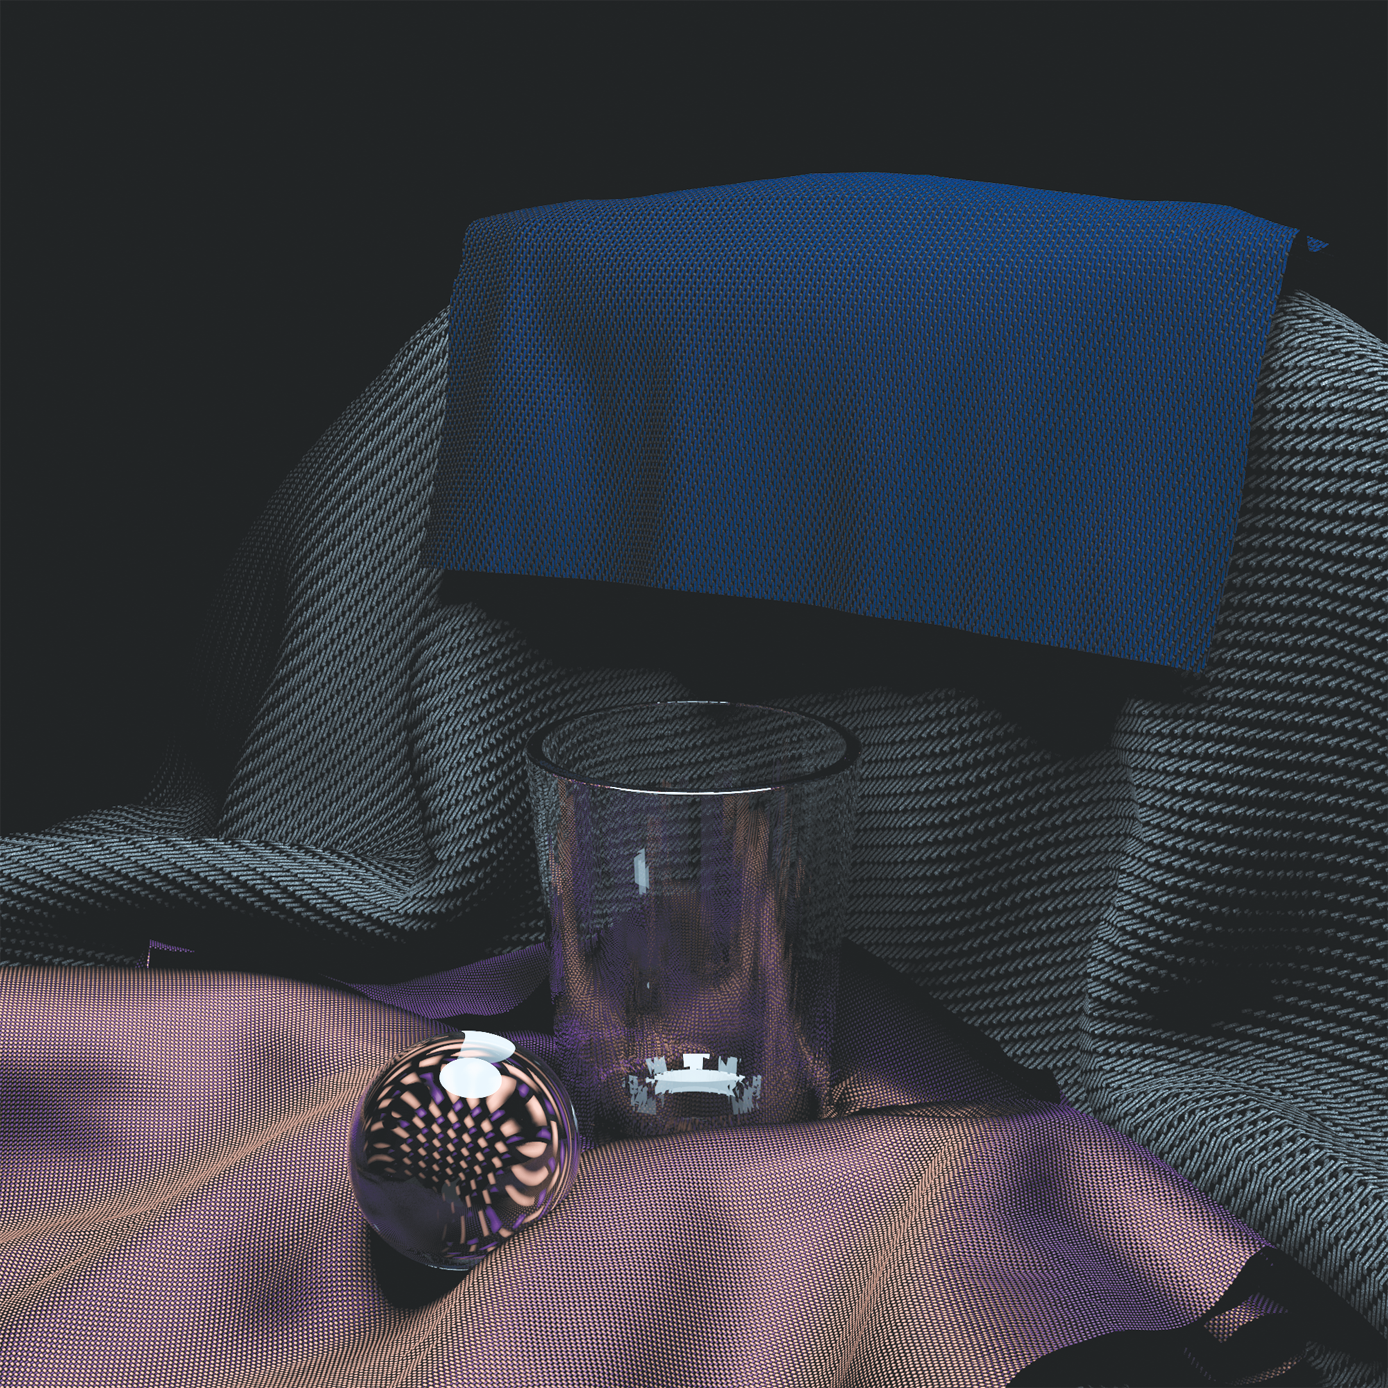
\includegraphics[width=\linewidth]{chap01/cloth.png}
    \caption{Lingfeng Yang实现了双向纹理函数来模拟布料的外观,
        添加了解析的自阴影模型,
        渲染了这张2009斯坦福大学CS348b渲染竞赛一等奖图像。}
    \label{fig:1.13}
\end{figure}

\subsection{执行阶段}\label{sub:执行阶段}

pbrt在概念上可分为两个执行阶段。
首先,解析用户提供的场景描述文件。
场景描述是一个文本文件,
指定了构成场景的几何形状及其材质属性、
对其照明的光源、虚拟相机在场景中的摆放位置、
整个系统所用的各个算法的参数等。
输入文件的每个语句都直接映射到
附录第\refchap{场景描述接口}
\sidenote{译者注:原书此处似乎链接错误,已纠正。}
中的一个例程;
这些例程包含了描述场景的程序接口。
场景文件格式的文档详见pbrt网站\href{https://pbrt.org/}{\ttfamily pbrt.org}。

解析阶段的最终结果是类\refvar{Scene}{}和\refvar{Integrator}{}的实例。
\refvar{Scene}{}包含了场景内容(几何物体、光源等)的表示,
\refvar{Integrator}{}则实现渲染它的算法。称之为\keyindex{积分器}{integrator}{}就是因为
它的主要任务是计算\refeq{1.1}的积分。

一旦指定好场景,第二执行阶段就开始了,执行主渲染循环。
pbrt通常把绝大部分运行时间都花在这个阶段,
本书大部分都在讲解执行这一阶段的代码。
渲染循环由\refvar{Integrator::Render}{()}的
实现来执行,它是\refsub{主渲染循环}的重点。

本章将介绍\refvar{Integrator}{}的一个特定子类,
称为\refvar{SamplerIntegrator}{},
其{\ttfamily Render()}方法为大量建模成像过程的光线
确定到达虚拟胶片平面的光量。
在计算完所有这些胶片样本的贡献后,把最终图像写入文件。
内存里的场景描述数据被释放,
系统从场景描述文件恢复处理语句直到没有剩余,
如果需要,用户可以指定下一个要渲染的场景。

\begin{figure}[htbp]
    \centering\includegraphics[width=\linewidth]{chap01/furrydog.png}
    \caption{Jared Jacobs和Michael Turitzin为pbrt增加了
        Kajiya和Kay基于纹素的毛发渲染算法\citep{10.1145/74334.74361}并渲染了该图像,
        狗毛和粗毛地毯都是用纹素毛发算法渲染的。}
    \label{fig:1.14}
\end{figure}

\reffig{1.15}和\reffig{1.16}由\emph{LuxRender}渲染,
它是最初基于本书第一版pbrt源码的GPL许可的基于物理的渲染系统
(关于\emph{LuxRender}的更多信息详见\url{https://luxcorerender.org}
\sidenote{译者注:\emph{LuxRender}已更名为\emph{LuxCoreRender}且
    迁移到了新网址。此处已更正了网址。})。

\begin{figure}[htbp]
    \centering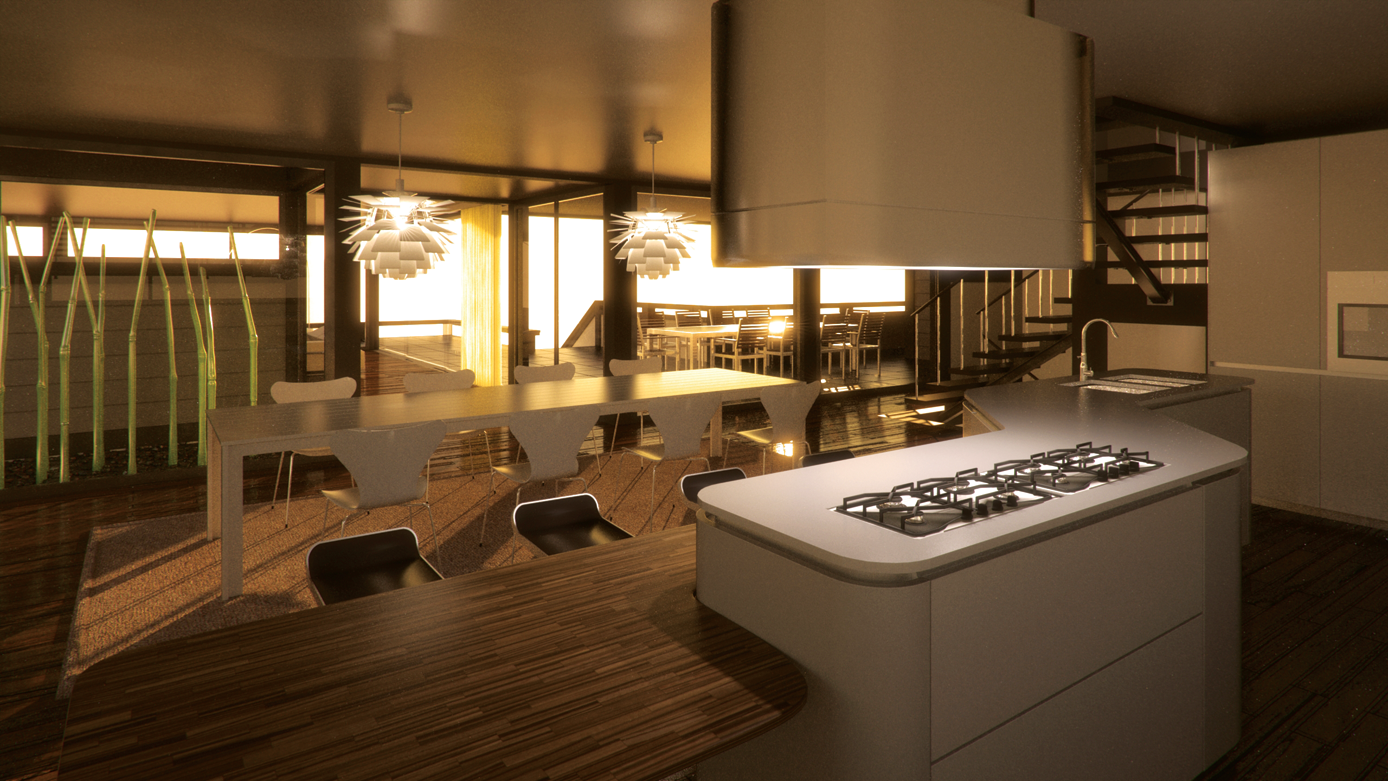
\includegraphics[width=\linewidth]{chap01/measure-one180-cut1260.png}
    \caption{Florent Boyer渲染了这个当代室内场景。
        该图像由\emph{LuxRender}渲染,它是最初
        基于pbrt源码的GPL许可的基于物理的渲染系统。
        建模和纹理由Blender完成。}
    \label{fig:1.15}
\end{figure}

\begin{figure}[htbp]
    \centering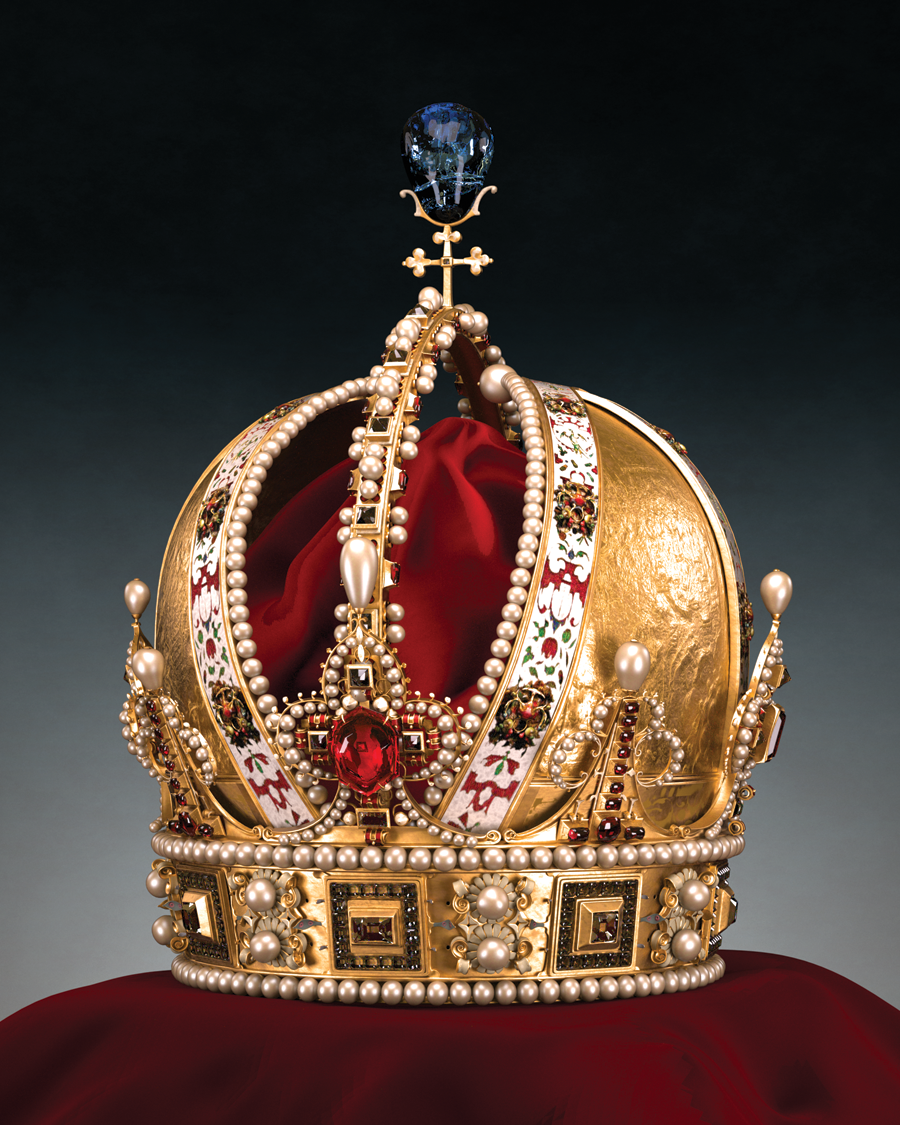
\includegraphics[width=\linewidth]{chap01/crown.png}
    \caption{Martin Lubich构建了这个奥地利皇冠的场景
        并用pbrt代码库的开源分支\emph{LuxRender}渲染了它。
        该场景由Blender建模,包含约一百八十万个顶点。
        它由具备基于真实世界光源测量数据的发射光谱的六个面光源照明,
        在四核CPU上对每个像素做1280次采样经73小时的计算完成渲染。
        包括可下载的Blender场景文件在内的更多信息
        详见Martin的网站\url{www.loramel.net}。}
    \label{fig:1.16}
\end{figure}

\subsection{场景表示}\label{sub:场景表示}
pbrt的函数\refvar{main}{()}可在
文件\href{https://github.com/mmp/pbrt-v3/tree/master/src/main/pbrt.cpp}{\ttfamily main/pbrt.cpp}内找到。
该函数很简单;
它首先循环读取{\ttfamily argv}中的命令行参数,
初始化结构体{\ttfamily Options}中的值并
保存参数中的文件名。
运行pbrt时带命令行参数{\ttfamily {-}{-}help}会
打印所有可指定的命令行选项。
解析命令行参数的代码片\refcode{Process command-line arguments}{}很简单,
故本书不再介绍\sidenote{译者注:我还是把它搬上来了。}。

选项结构体随后传入函数\refvar{pbrtInit}{()},做全系统初始化。
函数\refvar{main}{()}再解析给定场景描述,
创建\refvar{Scene}{}和\refvar{Integrator}{}。
\refvar{pbrtCleanup}{()}在系统完成所有渲染后退出前做最后的清理工作。

函数\refvar{pbrtInit}{()}和\refvar{pbrtCleanup}{()}出现在
页边空白处的迷你索引内,还注明了真正定义它们的页数。
每页的迷你索引都指向了所用的几乎所有函数、类、方法和成员变量的定义
\sidenote{译者注:在线版已经全部改用超链接了。翻译时尽力还原了在线版的跳转功能。试试看吧!}。
\begin{lstlisting}
`\initcode{Main program}{=}`
int `\initvar{main}{}`(int argc, char *argv[]) {
    Options options;
    std::vector<std::string> filenames;
    `\refcode{Process command-line arguments}{}`
    `\refvar{pbrtInit}{}`(options);
    `\refcode{Process scene description}{}`
    `\refvar{pbrtCleanup}{}`();
    return 0;
}
\end{lstlisting}
其中
\begin{lstlisting}
`\initcode{Process command-line arguments}{=}`
for (int i = 1; i < argc; ++i) {
    if (!strcmp(argv[i], "--ncores") || !strcmp(argv[i], "--nthreads"))
        options.nThreads = atoi(argv[++i]);
    else if (!strcmp(argv[i], "--outfile")) options.imageFile = argv[++i];
    else if (!strcmp(argv[i], "--quick")) options.quickRender = true;
    else if (!strcmp(argv[i], "--quiet")) options.quiet = true;
    else if (!strcmp(argv[i], "--verbose")) options.verbose = true;
    else if (!strcmp(argv[i], "--help") || !strcmp(argv[i], "-h")) {
        printf("usage: pbrt [--nthreads n] [--outfile filename] [--quick] [--quiet] "
               "[--verbose] [--help] <filename.pbrt> ...\n");
        return 0;
    }
    else filenames.push_back(argv[i]);
}
\end{lstlisting}

如果运行pbrt时没有提供输入文件名,
则它会从标准输入读取场景描述。
否则它就遍历提供的文件名,依次处理每个文件。
\begin{lstlisting}
`\initcode{Process scene description}{=}`
if (filenames.size() == 0) {
    `\refcode{Parse scene from standard input}{}`
} else {
    `\refcode{Parse scene from input files}{}`
}
\end{lstlisting}
函数{\initvar{ParseFile}{()}}或从标准输入或磁盘文件读入并解析场景描述文件;
如果无法打开文件则返回{\ttfamily false}。
本书不介绍解析场景描述文件的机制;
解析器的实现可在文件\href{https://github.com/mmp/pbrt-v3/blob/master/src/core/parser.h}{\ttfamily core/parser.h}和
\href{https://github.com/mmp/pbrt-v3/blob/master/src/core/parser.cpp}{\ttfamily core/parser.cpp}中找到
\sidenote{译者注:此处已更正文件名,因为原书给出的文件名已经失效了。}。
想要了解解析子系统但不熟悉这些工具的读者可以参阅Levine、Mason和Brown的著作\citep{10.5555/136311}。

我们遵循的UNIX习惯用法,以名为“{\ttfamily -}”的文件表示标准输入:
\begin{lstlisting}
`\initcode{Parse scene from standard input}{=}`
`\refvar{ParseFile}{}`("-");
\end{lstlisting}

如果无法打开特定的输入文件,则\refvar{Error}{()}例程会将此信息报告给用户。
\refvar{Error}{()}使用和{\ttfamily printf()}相同的格式化字符串语义。
\begin{lstlisting}
`\initcode{Parse scene from input files}{=}`
for (const std::string &f : filenames)
    if (!`\refvar{ParseFile}{}`(f))
        `\refvar{Error}{}`("Couldn't open scene file \"%s\"", f.c_str());
\end{lstlisting}

解析完场景文件后就创建表示场景中光源和几何图元的对象。
它们都存于\refvar{Scene}{}对象中,
由附录\refsub{世界端和渲染}的方法\refvar{RenderOptions::MakeScene}{()}创建。
类\refvar{Scene}{}在\href{https://github.com/mmp/pbrt-v3/tree/master/src/core/scene.h}{\ttfamily core/scene.h}中
声明并在\href{https://github.com/mmp/pbrt-v3/tree/master/src/core/scene.cpp}{\ttfamily core/scene.cpp}中定义。
\begin{lstlisting}
`\initcode{Scene Declarations}{=}`
class `\initvar{Scene}{}` {
public:
    `\refcode{Scene Public Methods}{}`
    `\refcode{Scene Public Data}{}`
private:
    `\refcode{Scene Private Data}{}`
};
\end{lstlisting}

\begin{lstlisting}
`\initcode{Scene Public Methods}{=}\initnext{ScenePublicMethods}`
`\refvar{Scene}{}`(std::shared_ptr<`\refvar{Primitive}{}`> `\refvar{aggregate}{}`,
      const std::vector<std::shared_ptr<`\refvar{Light}{}`>> &`\refvar{lights}{}`)
    : `\refvar{lights}{}`(`\refvar{lights}{}`), `\refvar{aggregate}{}`(`\refvar{aggregate}{}`) {
    `\refcode{Scene Constructor Implementation}{}`
}
\end{lstlisting}

场景中每个光源都由\refvar{Light}{}对象表示,
指定灯光的形状和发射能量的分布。
\refvar{Scene}{}用C++标准库中{\ttfamily shared\_ptr}实例
的一个{\ttfamily vector}来存储所有光源。
pbrt用共享指针\sidenote{译者注:原文shared pointers,是一种智能指针。}跟踪
其他实例对于对象的引用计数。
当最后一个持有引用的实例(例如这里的\refvar{Scene}{})被销毁时,
引用计数减到零,\refvar{Light}{}就可以安全释放了,而且是自动的。

尽管一些渲染器支持每个几何对象有单独的光源列表,
允许一个光源只照明场景中一部分物体,
但这种做法不符合pbrt采用的基于物理的渲染方法,
所以对于每个场景pbrt只支持单个全局列表。
系统的许多部分都需要获取光源,
所以\refvar{Scene}{}把它们置为公有成员变量。
\begin{lstlisting}
`\initcode{Scene Public Data}{=}`
std::vector<std::shared_ptr<`\refvar{Light}{}`>> `\initvar{lights}{}`;
\end{lstlisting}

场景中每个几何对象都由\refvar{Primitive}{}表示,结合了两个对象:
指定其几何结构的\refvar{Shape}{}和描述其外观
(例如物体的颜色、是否具有暗淡或光泽饰面)的\refvar{Material}{}。
所有几何图元都集中到\refvar{Scene}{}的
成员变量\refvar[aggregate]{Scene::aggregate}{}这一
单个\refvar{Primitive}{}聚合体中。
这个聚合体是一种特殊的图元,它自己持有许多对其他图元的引用。
因为它实现了\refvar{Primitive}{}接口,
所以从单个图元到系统其余部分似乎没什么区别。
聚合体的实现用加速的数据结构存储了所有场景图元,
减少对远离给定光线的图元做不必要的光线交点测试量。
\begin{lstlisting}
`\initcode{Scene Private Data}{=}\initnext{ScenePrivateData}`
std::shared_ptr<`\refvar{Primitive}{}`> `\initvar{aggregate}{}`;
\end{lstlisting}
构造函数把场景几何的边框缓存到成员变量{\ttfamily worldBound}中。
\begin{lstlisting}
`\initcode{Scene Constructor Implementation}{=}\initnext{SceneConstructorImplementation}`
`\refvar{worldBound}{}` = aggregate->`\refvar{WorldBound}{}`();
\end{lstlisting}
\begin{lstlisting}
`\refcode{Scene Private Data}{+=}\lastcode{ScenePrivateData}`
`\refvar{Bounds3f}{}` `\initvar{worldBound}{}`;
\end{lstlisting}
可通过方法{\ttfamily WorldBound()}获取该边界。
\begin{lstlisting}
`\refcode{Scene Public Methods}{+=}\lastcode{ScenePublicMethods}`
const `\refvar{Bounds3f}{}` &WorldBound() const { return `\refvar{worldBound}{}`; }
\end{lstlisting}

一些光源实现发现在定义场景后开始渲染前做一些额外的初始化很有用。
\refvar{Scene}{}的构造函数调用其方法\refvar{Preprocess}{()}来允许它们这么做。
\begin{lstlisting}
`\refcode{Scene Constructor Implementation}{+=}\lastcode{SceneConstructorImplementation}`
for (const auto &light : `\refvar{lights}{}`)
    light->`\refvar{Preprocess}{}`(*this);
\end{lstlisting}

\refvar{Scene}{}类提供两个与光线-图元交点相关的方法。
它的\refvar[Scene::Intersect]{Intersect}{()}方法跟随给定光线到场景中并
返回表示光线是否与某一图元相交的布尔值。
如果是,它便把沿光线最近交点的信息填入提供的结构体\refvar{SurfaceInteraction}{}。
结构体\refvar{SurfaceInteraction}{}将在\refsec{图元接口与几何图元}定义。
\begin{lstlisting}
`\initcode{Scene Method Definitions}{=}\initnext{SceneMethodDefinitions}`
bool `\refvar{Scene}{}`::`\refvar[Intersect]{\initvar[Scene::Intersect]{Intersect}{}}{}`(const `\refvar{Ray}{}` &ray, `\refvar{SurfaceInteraction}{}` *isect) const {
    return `\refvar{aggregate}{}`->`\refvar{Intersect}{}`(ray, isect);
}
\end{lstlisting}
一个紧密相关的方法是\refvar{Scene::IntersectP}{()},
它沿光线检查交点的存在性但不返回任何关于这些交点的信息。
因为这个例程不需要搜索最近的交点或计算任何关于交点的额外信息,
所以它一般比\refvar{Scene::Intersect}{()}更高效。
这个例程用于阴影射线。
\begin{lstlisting}
`\refcode{Scene Method Definitions}{+=}\lastnext{SceneMethodDefinitions}`
bool `\refvar{Scene}{}`::`\refvar[IntersectP]{\initvar[Scene::IntersectP]{IntersectP}{}}{}`(const `\refvar{Ray}{}` &ray) const {
    return `\refvar{aggregate}{}`->`\refvar{IntersectP}{}`(ray);
}
\end{lstlisting}

\subsection{积分器接口与采样积分器}\label{sub:积分器接口与采样积分器}
渲染一幅场景图像由实现了\refvar{Integrator}{}接口的类的实例负责。
抽象基类\refvar{Integrator}{}定义了任何积分器必须提供的方法\refvar[Integrator::Render]{Render}{()}。
本节我们将定义一个\refvar{Integrator}{}的实现,即\refvar{SamplerIntegrator}{}。
在\href{https://github.com/mmp/pbrt-v3/tree/master/src/core/integrator.h}{\ttfamily core/integrator.h}中
定义了基本积分器接口,
积分器使用的一些实用函数在\href{https://github.com/mmp/pbrt-v3/blob/master/src/core/integrator.cpp}{\ttfamily core/integrator.cpp}中。
不同积分器的实现在目录\href{https://github.com/mmp/pbrt-v3/tree/master/src/integrators}{\ttfamily integrators}中。
\begin{lstlisting}
`\initcode{Integrator Declarations}{=}`
class `\initvar{Integrator}{}` {
public:
    `\refcode{Integrator Interface}{}`
};
\end{lstlisting}

\refvar{Integrator}{}必须提供方法\refvar[Integrator::Render]{Render}{()};
它利用传入的\refvar{Scene}{}引用计算一幅场景图像,
或者更一般地说,一组场景光照的度量。
其接口专门保持高度一般性以便允许各种实现——
例如可以把\refvar{Integrator}{}实现成只度量
分布于场景中的一组稀疏位置,而不是生成常规的2D图像。
\begin{lstlisting}
`\initcode{Integrator Interface}{=}`
virtual void `\initvar[Integrator::Render]{Render}{}`(const `\refvar{Scene}{}` &scene) = 0;
\end{lstlisting}

本章中,我们的重点是\refvar{Integrator}{}的一个子类\refvar{SamplerIntegrator}{},
以及实现了\refvar{SamplerIntegrator}{}接口的\refvar{WhittedIntegrator}{}。
(\refvar{SamplerIntegrator}{}的其他实现
会在第\refchap{光传输I:表面反射}和\refchap{光传输II:体积渲染}介绍;
第\refchap{光传输III:双向方法}的积分器直接从\refvar{Integrator}{}继承。)
\refvar{SamplerIntegrator}{}的名字源自其渲染过程
由来自\refvar{Sampler}{}的\keyindex{样本}{sample}{}流驱动的;
每个这样的样本都标识了图像上的一点,
让积分器计算到达该点以构成图像的光量。
\begin{lstlisting}
`\initcode{SamplerIntegrator Declarations}{=}`
class `\initvar{SamplerIntegrator}{}` : public `\refvar{Integrator}{}` {
public:
    `\refcode{SamplerIntegrator Public Methods}{}`
protected:
    `\refcode{SamplerIntegrator Protected Data}{}`
private:
    `\refcode{SamplerIntegrator Private Data}{}`
};
\end{lstlisting}

\refvar{SamplerIntegrator}{}保存了指向\refvar{Sampler}{}的指针。
采样器看似存在感低,但它的实现会极大影响系统生成图像的质量。
首先,采样器负责选取光线要追踪的图像平面上的点。
其次,它负责为积分器提供用于计算光传输积分即\refeq{1.1}的值所需的采样位置。
例如,一些积分器需要对光源选取随机位置来计算来自面光源的照明。
生成分布良好的样本在渲染过程中很重要,会极大影响整体效率;
这是第\refchap{采样与重构}的主要内容。
\begin{lstlisting}
`\initcode{SamplerIntegrator Private Data}{=}`
std::shared_ptr<`\refvar{Sampler}{}`> `\initvar{sampler}{}`;
\end{lstlisting}

对象\refvar{Camera}{}控制视角和透镜参数,例如位置、朝向、焦点和视野。
\refvar{Camera}{}内的成员变量\refvar{Film}{}执行图像存储。
\refvar{Camera}{}类将在第\refchap{相机模型}介绍,
\refvar{Film}{}将在\refsec{胶片与成像管道}介绍。
\refvar{Film}{}负责把最终图像写入文件并可能在完成计算后在屏幕上将其显示出来。
\begin{lstlisting}
`\initcode{SamplerIntegrator Protected Data}{=}`
std::shared_ptr<const `\refvar{Camera}{}`> `\initvar{camera}{}`;
\end{lstlisting}

\refvar{SamplerIntegrator}{}构造函数在成员变量中保存了指向这些对象的指针。
它在被\refvar{pbrtWorldEnd}{()}调用的
方法\refvar{RenderOptions::MakeIntegrator}{()}里创建,
而\refvar{pbrtWorldEnd}{()}在输入文件解析器
完成对输入文件的场景描述解析并准备渲染场景时被调用。
\begin{lstlisting}
`\initcode{SamplerIntegrator Public Methods}{=}\initnext{SamplerIntegratorPublicMethods}`
`\refvar{SamplerIntegrator}{}`(std::shared_ptr<const `\refvar{Camera}{}`> `\refvar{camera}{}`,
        std::shared_ptr<`\refvar{Sampler}{}`> `\refvar{sampler}{}`)
    : `\refvar{camera}{}`(`\refvar{camera}{}`), `\refvar{sampler}{}`(`\refvar{sampler}{}`) { }
\end{lstlisting}

\refvar{SamplerIntegrator}{}可选实现方法\refvar[SamplerIntegrator::Preprocess]{Preprocess}{()}。
它在\refvar{Scene}{}完全初始化后被调用,
并给积分器机会完成依赖于场景的计算,
例如分配依赖于场景光源数目的额外数据结构,
或者预计算场景中辐射分布的大致表示。
在这里不需要做任何事的实现可以将这个方法留为未实现状态。
\begin{lstlisting}
`\refcode{SamplerIntegrator Public Methods}{=}\lastnext{SamplerIntegratorPublicMethods}`
virtual void `\initvar[SamplerIntegrator::Preprocess]{Preprocess}{}`(const `\refvar{Scene}{}` &scene, `\refvar{Sampler}{}` &sampler) { }
\end{lstlisting}

\subsection{主渲染循环}\label{sub:主渲染循环}
完成\refvar{Scene}{}和\refvar{Integrator}{}的分配与初始化后,
调用方法\refvar{Integrator::Render}{()},
开始pbrt的第二执行阶段:主渲染循环。
在\refvar{SamplerIntegrator}{}对该方法的实现中,
对于图像平面上一系列位置中的每一个,
该方法用\refvar{Camera}{}和\refvar{Sampler}{}生成到场景中的光线,
再用方法{\ttfamily Li()}确定沿该光线到达图像平面的光量。
该值传入\refvar{Film}{},记录下光的贡献度。
\reffig{1.17}总结了该方法用到的主要类和它们之间的数据流。
\begin{figure}[htbp]
    \centering%LaTeX with PSTricks extensions
%%Creator: Inkscape 1.0.1 (3bc2e813f5, 2020-09-07)
%%Please note this file requires PSTricks extensions
\psset{xunit=.5pt,yunit=.5pt,runit=.5pt}
\begin{pspicture}(893.08001709,262.91000366)
{
\newrgbcolor{curcolor}{0.80000001 0.80000001 0.80000001}
\pscustom[linestyle=none,fillstyle=solid,fillcolor=curcolor]
{
\newpath
\moveto(11.6500001,262.91000366)
\lineto(109.81000376,262.91000366)
\curveto(112.58000376,262.91000366)(114.81000376,260.68000366)(114.81000376,257.91000366)
\lineto(114.81000376,236.75000381)
\curveto(114.81000376,233.98000381)(112.58000376,231.75000381)(109.81000376,231.75000381)
\lineto(11.6500001,231.75000381)
\curveto(8.8800001,231.75000381)(6.6500001,233.98000381)(6.6500001,236.75000381)
\lineto(6.6500001,257.91000366)
\curveto(6.6500001,260.68000366)(8.8800001,262.91000366)(11.6500001,262.91000366)
\closepath
}
}
{
\newrgbcolor{curcolor}{0.80000001 0.80000001 0.80000001}
\pscustom[linestyle=none,fillstyle=solid,fillcolor=curcolor]
{
\newpath
\moveto(253.1499939,262.91000366)
\lineto(338.71999359,262.91000366)
\curveto(341.48999359,262.91000366)(343.71999359,260.68000366)(343.71999359,257.91000366)
\lineto(343.71999359,236.75000381)
\curveto(343.71999359,233.98000381)(341.48999359,231.75000381)(338.71999359,231.75000381)
\lineto(253.1499939,231.75000381)
\curveto(250.3799939,231.75000381)(248.1499939,233.98000381)(248.1499939,236.75000381)
\lineto(248.1499939,257.91000366)
\curveto(248.1499939,260.68000366)(250.3799939,262.91000366)(253.1499939,262.91000366)
\closepath
}
}
{
\newrgbcolor{curcolor}{0.80000001 0.80000001 0.80000001}
\pscustom[linestyle=none,fillstyle=solid,fillcolor=curcolor]
{
\newpath
\moveto(45.43999863,139.91000366)
\lineto(395.49999619,139.91000366)
\curveto(398.26999619,139.91000366)(400.49999619,137.68000366)(400.49999619,134.91000366)
\lineto(400.49999619,113.75000381)
\curveto(400.49999619,110.98000381)(398.26999619,108.75000381)(395.49999619,108.75000381)
\lineto(45.43999863,108.75000381)
\curveto(42.66999863,108.75000381)(40.43999863,110.98000381)(40.43999863,113.75000381)
\lineto(40.43999863,134.91000366)
\curveto(40.43999863,137.68000366)(42.66999863,139.91000366)(45.43999863,139.91000366)
\closepath
}
}
{
\newrgbcolor{curcolor}{0.80000001 0.80000001 0.80000001}
\pscustom[linestyle=none,fillstyle=solid,fillcolor=curcolor]
{
\newpath
\moveto(189.27999878,31.16000366)
\lineto(249.93000031,31.16000366)
\curveto(252.70000031,31.16000366)(254.93000031,28.93000366)(254.93000031,26.16000366)
\lineto(254.93000031,5.00000381)
\curveto(254.93000031,2.23000381)(252.70000031,0.00000381)(249.93000031,0.00000381)
\lineto(189.27999878,0.00000381)
\curveto(186.50999878,0.00000381)(184.27999878,2.23000381)(184.27999878,5.00000381)
\lineto(184.27999878,26.16000366)
\curveto(184.27999878,28.93000366)(186.50999878,31.16000366)(189.27999878,31.16000366)
\closepath
}
}
{
\newrgbcolor{curcolor}{0.80000001 0.80000001 0.80000001}
\pscustom[linestyle=none,fillstyle=solid,fillcolor=curcolor]
{
\newpath
\moveto(588.40002441,143.66000366)
\lineto(888.08001709,143.66000366)
\curveto(890.85001709,143.66000366)(893.08001709,141.43000366)(893.08001709,138.66000366)
\lineto(893.08001709,117.50000381)
\curveto(893.08001709,114.73000381)(890.85001709,112.50000381)(888.08001709,112.50000381)
\lineto(588.40002441,112.50000381)
\curveto(585.63002441,112.50000381)(583.40002441,114.73000381)(583.40002441,117.50000381)
\lineto(583.40002441,138.66000366)
\curveto(583.40002441,141.43000366)(585.63002441,143.66000366)(588.40002441,143.66000366)
\closepath
}
}
{
\newrgbcolor{curcolor}{0 0 0}
\pscustom[linewidth=1,linecolor=curcolor]
{
\newpath
\moveto(58.49000168,231.00000381)
\lineto(139.80999756,148.27000427)
}
}
{
\newrgbcolor{curcolor}{0 0 0}
\pscustom[linestyle=none,fillstyle=solid,fillcolor=curcolor]
{
\newpath
\moveto(132.44,147.92000366)
\lineto(139.35,148.74000366)
\lineto(140.29,155.63000366)
\lineto(145.49,142.50000366)
\closepath
}
}
{
\newrgbcolor{curcolor}{0.65098041 0.65098041 0.65098041}
\pscustom[linestyle=none,fillstyle=solid,fillcolor=curcolor]
{
\newpath
\moveto(144.57,143.43000366)
\lineto(139.8,148.29000366)
\lineto(134.39,147.65000366)
\closepath
}
}
{
\newrgbcolor{curcolor}{0.40000001 0.40000001 0.40000001}
\pscustom[linestyle=none,fillstyle=solid,fillcolor=curcolor]
{
\newpath
\moveto(139.8,148.29000366)
\lineto(140.53,153.68000366)
\lineto(144.57,143.43000366)
\closepath
}
}
{
\newrgbcolor{curcolor}{0 0 0}
\pscustom[linewidth=1,linecolor=curcolor]
{
\newpath
\moveto(251.97000122,141.52000427)
\lineto(287.11999512,221.98000336)
}
}
{
\newrgbcolor{curcolor}{0 0 0}
\pscustom[linestyle=none,fillstyle=solid,fillcolor=curcolor]
{
\newpath
\moveto(290.2,215.28000366)
\lineto(286.86,221.38000366)
\lineto(280.11,219.68000366)
\lineto(290.37,229.40000366)
\closepath
}
}
{
\newrgbcolor{curcolor}{0.65098041 0.65098041 0.65098041}
\pscustom[linestyle=none,fillstyle=solid,fillcolor=curcolor]
{
\newpath
\moveto(289.84,228.20000366)
\lineto(287.11,221.96000366)
\lineto(289.72,217.19000366)
\closepath
}
}
{
\newrgbcolor{curcolor}{0.40000001 0.40000001 0.40000001}
\pscustom[linestyle=none,fillstyle=solid,fillcolor=curcolor]
{
\newpath
\moveto(289.84,228.20000366)
\lineto(287.11,221.96000366)
\lineto(281.84,220.63000366)
\closepath
}
}
{
\newrgbcolor{curcolor}{0 0 0}
\pscustom[linewidth=1,linecolor=curcolor]
{
\newpath
\moveto(285.20999146,148.95000458)
\lineto(320.35998535,229.41000366)
}
}
{
\newrgbcolor{curcolor}{0 0 0}
\pscustom[linestyle=none,fillstyle=solid,fillcolor=curcolor]
{
\newpath
\moveto(292.22,151.24000366)
\lineto(285.47,149.54000366)
\lineto(282.13,155.65000366)
\lineto(281.96,141.52000366)
\closepath
}
}
{
\newrgbcolor{curcolor}{0.65098041 0.65098041 0.65098041}
\pscustom[linestyle=none,fillstyle=solid,fillcolor=curcolor]
{
\newpath
\moveto(282.49,142.72000366)
\lineto(285.22,148.96000366)
\lineto(290.49,150.30000366)
\closepath
}
}
{
\newrgbcolor{curcolor}{0.40000001 0.40000001 0.40000001}
\pscustom[linestyle=none,fillstyle=solid,fillcolor=curcolor]
{
\newpath
\moveto(282.61,153.74000366)
\lineto(282.49,142.72000366)
\lineto(285.22,148.96000366)
\closepath
}
}
{
\newrgbcolor{curcolor}{0 0 0}
\pscustom[linewidth=1,linecolor=curcolor]
{
\newpath
\moveto(220.03999329,108)
\lineto(220.03999329,40.3500061)
}
}
{
\newrgbcolor{curcolor}{0 0 0}
\pscustom[linestyle=none,fillstyle=solid,fillcolor=curcolor]
{
\newpath
\moveto(214.53,45.26000366)
\lineto(220.04,41.00000366)
\lineto(225.54,45.26000366)
\lineto(220.04,32.25000366)
\closepath
}
}
{
\newrgbcolor{curcolor}{0.65098041 0.65098041 0.65098041}
\pscustom[linestyle=none,fillstyle=solid,fillcolor=curcolor]
{
\newpath
\moveto(220.04,33.56000366)
\lineto(220.04,40.37000366)
\lineto(215.73,43.70000366)
\closepath
}
}
{
\newrgbcolor{curcolor}{0.40000001 0.40000001 0.40000001}
\pscustom[linestyle=none,fillstyle=solid,fillcolor=curcolor]
{
\newpath
\moveto(224.33,43.70000366)
\lineto(220.04,33.56000366)
\lineto(220.04,40.37000366)
\closepath
}
}
{
\newrgbcolor{curcolor}{0 0 0}
\pscustom[linewidth=1,linecolor=curcolor]
{
\newpath
\moveto(404.23999023,132)
\lineto(570.14001465,132)
}
}
{
\newrgbcolor{curcolor}{0 0 0}
\pscustom[linestyle=none,fillstyle=solid,fillcolor=curcolor]
{
\newpath
\moveto(565.23,126.49000366)
\lineto(569.49,132.00000366)
\lineto(565.23,137.50000366)
\lineto(578.24,132.00000366)
\closepath
}
}
{
\newrgbcolor{curcolor}{0.65098041 0.65098041 0.65098041}
\pscustom[linestyle=none,fillstyle=solid,fillcolor=curcolor]
{
\newpath
\moveto(576.93,132.00000366)
\lineto(570.12,132.00000366)
\lineto(566.79,127.69000366)
\closepath
}
}
{
\newrgbcolor{curcolor}{0.40000001 0.40000001 0.40000001}
\pscustom[linestyle=none,fillstyle=solid,fillcolor=curcolor]
{
\newpath
\moveto(566.79,136.29000366)
\lineto(576.93,132.00000366)
\lineto(570.12,132.00000366)
\closepath
}
}
{
\newrgbcolor{curcolor}{0 0 0}
\pscustom[linewidth=1,linecolor=curcolor]
{
\newpath
\moveto(413.83999634,117.75)
\lineto(579.73999023,117.75)
}
}
{
\newrgbcolor{curcolor}{0 0 0}
\pscustom[linestyle=none,fillstyle=solid,fillcolor=curcolor]
{
\newpath
\moveto(418.75,112.24000366)
\lineto(414.5,117.75000366)
\lineto(418.75,123.25000366)
\lineto(405.74,117.75000366)
\closepath
}
}
{
\newrgbcolor{curcolor}{0.65098041 0.65098041 0.65098041}
\pscustom[linestyle=none,fillstyle=solid,fillcolor=curcolor]
{
\newpath
\moveto(413.87,117.75000366)
\lineto(417.2,113.44000366)
\lineto(407.05,117.75000366)
\closepath
}
}
{
\newrgbcolor{curcolor}{0.40000001 0.40000001 0.40000001}
\pscustom[linestyle=none,fillstyle=solid,fillcolor=curcolor]
{
\newpath
\moveto(413.87,117.75000366)
\lineto(417.2,122.04000366)
\lineto(407.05,117.75000366)
\closepath
}
}
{
\newrgbcolor{curcolor}{0 0 0}
\pscustom[linestyle=none,fillstyle=solid,fillcolor=curcolor]
{
\newpath
\moveto(18.83423174,243.34563524)
\curveto(18.64673203,243.12341337)(18.4939545,242.98105249)(18.37589913,242.91855258)
\curveto(18.26478819,242.85605268)(18.12589952,242.82480273)(17.95923312,242.82480273)
\curveto(17.63284475,242.82480273)(17.36895627,242.93244145)(17.1675677,243.14771889)
\curveto(16.97312357,243.36994076)(16.8759015,243.73452352)(16.8759015,244.24146716)
\lineto(16.8759015,245.67896489)
\curveto(16.8759015,246.19285297)(16.97312357,246.55743573)(17.1675677,246.77271316)
\curveto(17.36895627,246.99493503)(17.63284475,247.10604597)(17.95923312,247.10604597)
\curveto(18.20923272,247.10604597)(18.41756573,247.04007385)(18.58423213,246.90812962)
\curveto(18.75784297,246.77618538)(18.8897872,246.55396351)(18.98006484,246.241464)
\curveto(19.07034248,245.93590893)(19.16409233,245.72757592)(19.2613144,245.61646499)
\curveto(19.46270297,245.40118755)(19.82034129,245.1824379)(20.33422937,244.96021603)
\curveto(20.84811745,244.73799415)(21.41061656,244.62688322)(22.0217267,244.62688322)
\curveto(22.97311409,244.62688322)(23.75436285,244.84910509)(24.365473,245.29354883)
\curveto(24.75436128,245.56438174)(24.94880541,245.89771454)(24.94880541,246.29354725)
\curveto(24.94880541,246.55743573)(24.85505556,246.80396311)(24.66755586,247.03312942)
\curveto(24.48005615,247.26924016)(24.17450108,247.46368429)(23.75089064,247.61646183)
\curveto(23.4731133,247.72062833)(22.8515865,247.86298922)(21.88631025,248.04354449)
\curveto(20.71964543,248.25882193)(19.83770237,248.51923818)(19.2404811,248.82479325)
\curveto(18.64325982,249.13034833)(18.17103834,249.5609032)(17.82381667,250.11645788)
\curveto(17.47659499,250.67201256)(17.30298416,251.27270606)(17.30298416,251.91853837)
\curveto(17.30298416,252.93937009)(17.73006681,253.83172979)(18.58423213,254.59561747)
\curveto(19.43839745,255.36644959)(20.54950681,255.75186565)(21.9175602,255.75186565)
\curveto(22.46617044,255.75186565)(22.97311409,255.68936575)(23.43839113,255.56436594)
\curveto(23.91061261,255.44631057)(24.33769527,255.26228309)(24.71963911,255.01228348)
\curveto(24.99741645,255.28311639)(25.27519379,255.41853284)(25.55297112,255.41853284)
\curveto(25.86547063,255.41853284)(26.11894245,255.3074219)(26.31338659,255.08520003)
\curveto(26.51477516,254.8699226)(26.61546945,254.50881205)(26.61546945,254.00186841)
\lineto(26.61546945,252.39770428)
\curveto(26.61546945,251.8838162)(26.51477516,251.51576123)(26.31338659,251.29353936)
\curveto(26.11894245,251.07826192)(25.86547063,250.9706232)(25.55297112,250.9706232)
\curveto(25.28908265,250.9706232)(25.05991635,251.05048418)(24.86547221,251.21020615)
\curveto(24.71269467,251.32826152)(24.59811152,251.56437226)(24.52172275,251.91853837)
\curveto(24.44533399,252.27270448)(24.34811192,252.5261763)(24.23005655,252.67895383)
\curveto(24.02866798,252.94284231)(23.72658512,253.16506418)(23.32380798,253.34561945)
\curveto(22.92103084,253.52617472)(22.45575379,253.61645235)(21.92797685,253.61645235)
\curveto(21.15714473,253.61645235)(20.54603459,253.43589708)(20.09464641,253.07478654)
\curveto(19.65020267,252.72062043)(19.4279808,252.34909324)(19.4279808,251.96020497)
\curveto(19.4279808,251.6963165)(19.51825843,251.43937246)(19.6988137,251.18937285)
\curveto(19.88631341,250.94631768)(20.15714631,250.75534576)(20.51131242,250.61645709)
\curveto(20.74742316,250.51923502)(21.41061656,250.36298527)(22.50089261,250.14770783)
\curveto(23.5981131,249.93243039)(24.43838955,249.69631966)(25.02172196,249.43937562)
\curveto(25.61199881,249.18243158)(26.10158137,248.77965444)(26.49046964,248.23104419)
\curveto(26.87935792,247.68243395)(27.07380206,247.0296572)(27.07380206,246.27271395)
\curveto(27.07380206,245.21716006)(26.70227486,244.3734114)(25.95922048,243.74146795)
\curveto(24.97311093,242.90813593)(23.71616847,242.49146993)(22.18839311,242.49146993)
\curveto(21.59811626,242.49146993)(21.02172828,242.56438648)(20.45922917,242.71021958)
\curveto(19.90367449,242.84910825)(19.36200868,243.06091347)(18.83423174,243.34563524)
\closepath
}
}
{
\newrgbcolor{curcolor}{0 0 0}
\pscustom[linestyle=none,fillstyle=solid,fillcolor=curcolor]
{
\newpath
\moveto(36.67795343,242.80396943)
\lineto(36.67795343,243.30396864)
\curveto(36.14323205,243.01924687)(35.55295521,242.80744165)(34.90712289,242.66855298)
\curveto(34.26129058,242.52271988)(33.67448595,242.44980332)(33.14670901,242.44980332)
\curveto(32.00087748,242.44980332)(31.0703234,242.75188618)(30.35504675,243.35605189)
\curveto(29.6397701,243.96716204)(29.28213178,244.64077209)(29.28213178,245.37688203)
\curveto(29.28213178,246.27271395)(29.73699217,247.10257375)(30.64671296,247.86646144)
\curveto(31.56337817,248.63729355)(32.82726507,249.02270961)(34.43837363,249.02270961)
\curveto(35.08420595,249.02270961)(35.83073254,248.95326527)(36.67795343,248.8143766)
\lineto(36.67795343,249.32479247)
\curveto(36.67795343,249.64423641)(36.53906476,249.90465266)(36.26128742,250.10604123)
\curveto(35.99045451,250.3074298)(35.469622,250.40812409)(34.69878989,250.40812409)
\curveto(34.06684644,250.40812409)(33.24740329,250.28312428)(32.24046044,250.03312468)
\curveto(31.86546103,249.94284704)(31.57379482,249.89770823)(31.36546182,249.89770823)
\curveto(31.08074005,249.89770823)(30.83768488,249.99840251)(30.6362963,250.19979108)
\curveto(30.44185217,250.40812409)(30.3446301,250.67201256)(30.3446301,250.9914565)
\curveto(30.3446301,251.17201177)(30.37935227,251.32826152)(30.4487966,251.46020576)
\curveto(30.51824094,251.59214999)(30.615463,251.6963165)(30.74046281,251.77270527)
\curveto(30.86546261,251.85603847)(31.12587887,251.95326054)(31.52171157,252.06437147)
\curveto(32.04948852,252.21020457)(32.58768211,252.32478773)(33.13629236,252.40812093)
\curveto(33.6849026,252.49839856)(34.18142959,252.54353738)(34.62587334,252.54353738)
\curveto(35.95226013,252.54353738)(36.98003628,252.25534339)(37.7092018,251.67895541)
\curveto(38.44531175,251.10951187)(38.81336672,250.3282631)(38.81336672,249.33520912)
\lineto(38.81336672,244.93938273)
\lineto(39.17794948,244.93938273)
\curveto(39.69183756,244.93938273)(40.05642031,244.83868844)(40.27169775,244.63729987)
\curveto(40.49391962,244.44285573)(40.60503056,244.18591169)(40.60503056,243.86646775)
\curveto(40.60503056,243.55396825)(40.49391962,243.29702421)(40.27169775,243.09563564)
\curveto(40.05642031,242.9011915)(39.69183756,242.80396943)(39.17794948,242.80396943)
\closepath
\moveto(36.67795343,246.62688006)
\curveto(35.82378811,246.79354646)(35.03559491,246.87687967)(34.31337383,246.87687967)
\curveto(33.44531965,246.87687967)(32.69879305,246.66507444)(32.07379403,246.241464)
\curveto(31.68490576,245.9706311)(31.49046162,245.69632597)(31.49046162,245.41854864)
\curveto(31.49046162,245.21716006)(31.58421147,245.05396588)(31.77171118,244.92896608)
\curveto(32.11893285,244.69979977)(32.59462655,244.58521662)(33.19879226,244.58521662)
\curveto(33.71268033,244.58521662)(34.29254053,244.6859109)(34.93837284,244.88729947)
\curveto(35.59114959,245.08868805)(36.17100978,245.36299317)(36.67795343,245.71021484)
\closepath
}
}
{
\newrgbcolor{curcolor}{0 0 0}
\pscustom[linestyle=none,fillstyle=solid,fillcolor=curcolor]
{
\newpath
\moveto(44.26127466,252.26228783)
\lineto(44.26127466,251.65812211)
\curveto(44.60849633,251.99839935)(44.92099584,252.23103787)(45.19877318,252.35603768)
\curveto(45.48349495,252.48798191)(45.80988333,252.55395403)(46.1779383,252.55395403)
\curveto(46.49043781,252.55395403)(46.7994651,252.47756526)(47.10502017,252.32478773)
\curveto(47.41057524,252.17201019)(47.70918588,251.94284389)(48.00085209,251.63728881)
\curveto(48.36890706,251.94284389)(48.74043425,252.16853797)(49.11543366,252.31437108)
\curveto(49.4973775,252.46714861)(49.88626578,252.54353738)(50.28209848,252.54353738)
\curveto(51.0737639,252.54353738)(51.716124,252.33173216)(52.20917877,251.90812172)
\curveto(52.86195552,251.35256704)(53.18834389,250.62340153)(53.18834389,249.72062517)
\lineto(53.18834389,244.93938273)
\curveto(53.63278764,244.93938273)(53.96264823,244.83868844)(54.17792566,244.63729987)
\curveto(54.3932031,244.4359113)(54.50084182,244.17896726)(54.50084182,243.86646775)
\curveto(54.50084182,243.55396825)(54.3932031,243.29702421)(54.17792566,243.09563564)
\curveto(53.96264823,242.9011915)(53.59806547,242.80396943)(53.08417739,242.80396943)
\lineto(51.0529306,242.80396943)
\lineto(51.0529306,249.54354212)
\curveto(51.0529306,249.86993049)(50.99390291,250.09562458)(50.87584755,250.22062438)
\curveto(50.75779218,250.34562419)(50.57723691,250.40812409)(50.33418173,250.40812409)
\curveto(50.098071,250.40812409)(49.87932134,250.34562419)(49.67793277,250.22062438)
\curveto(49.42098873,250.04701355)(49.10848923,249.72062517)(48.74043425,249.24145926)
\lineto(48.74043425,244.93938273)
\curveto(49.18487799,244.93938273)(49.51473858,244.83868844)(49.73001602,244.63729987)
\curveto(49.94529346,244.4359113)(50.05293218,244.17896726)(50.05293218,243.86646775)
\curveto(50.05293218,243.55396825)(49.94529346,243.29702421)(49.73001602,243.09563564)
\curveto(49.51473858,242.9011915)(49.15015583,242.80396943)(48.63626775,242.80396943)
\lineto(46.60502096,242.80396943)
\lineto(46.60502096,249.54354212)
\curveto(46.60502096,249.86298606)(46.54252106,250.08520793)(46.41752125,250.21020773)
\curveto(46.29946589,250.34215197)(46.11891061,250.40812409)(45.87585544,250.40812409)
\curveto(45.62585584,250.40812409)(45.37932845,250.3282631)(45.13627328,250.16854113)
\curveto(44.89321811,250.0157636)(44.6015519,249.70673631)(44.26127466,249.24145926)
\lineto(44.26127466,244.93938273)
\curveto(44.7057184,244.93938273)(45.03557899,244.83868844)(45.25085643,244.63729987)
\curveto(45.4730783,244.4359113)(45.58418924,244.17896726)(45.58418924,243.86646775)
\curveto(45.58418924,243.55396825)(45.4730783,243.29702421)(45.25085643,243.09563564)
\curveto(45.03557899,242.9011915)(44.67099624,242.80396943)(44.15710816,242.80396943)
\lineto(42.23002787,242.80396943)
\curveto(41.71613979,242.80396943)(41.35155703,242.9011915)(41.1362796,243.09563564)
\curveto(40.91405772,243.29702421)(40.80294679,243.55744046)(40.80294679,243.8768844)
\curveto(40.80294679,244.18938391)(40.91058551,244.44285573)(41.12586295,244.63729987)
\curveto(41.34114038,244.83868844)(41.67447319,244.93938273)(42.12586137,244.93938273)
\lineto(42.12586137,250.12687453)
\curveto(41.67447319,250.12687453)(41.34114038,250.22756882)(41.12586295,250.42895739)
\curveto(40.91058551,250.63034596)(40.80294679,250.88729)(40.80294679,251.1997895)
\curveto(40.80294679,251.51228901)(40.91405772,251.76576083)(41.1362796,251.96020497)
\curveto(41.35155703,252.16159354)(41.71613979,252.26228783)(42.23002787,252.26228783)
\closepath
}
}
{
\newrgbcolor{curcolor}{0 0 0}
\pscustom[linestyle=none,fillstyle=solid,fillcolor=curcolor]
{
\newpath
\moveto(57.70916996,243.98105091)
\lineto(57.70916996,240.48105643)
\lineto(58.99041794,240.48105643)
\curveto(59.50430602,240.48105643)(59.86888877,240.38383437)(60.08416621,240.18939023)
\curveto(60.30638808,239.98800166)(60.41749902,239.7275854)(60.41749902,239.40814146)
\curveto(60.41749902,239.09564196)(60.30638808,238.84217013)(60.08416621,238.647726)
\curveto(59.86888877,238.44633743)(59.50430602,238.34564314)(58.99041794,238.34564314)
\lineto(55.20917391,238.34564314)
\curveto(54.69528583,238.34564314)(54.32723086,238.44633743)(54.10500899,238.647726)
\curveto(53.88973155,238.84217013)(53.78209283,239.09564196)(53.78209283,239.40814146)
\curveto(53.78209283,239.7275854)(53.89320377,239.98800166)(54.11542564,240.18939023)
\curveto(54.33764751,240.38383437)(54.70223027,240.48105643)(55.20917391,240.48105643)
\lineto(55.57375667,240.48105643)
\lineto(55.57375667,250.12687453)
\lineto(55.20917391,250.12687453)
\curveto(54.69528583,250.12687453)(54.32723086,250.2240966)(54.10500899,250.41854074)
\curveto(53.88973155,250.61992931)(53.78209283,250.88034556)(53.78209283,251.1997895)
\curveto(53.78209283,251.51228901)(53.88973155,251.76576083)(54.10500899,251.96020497)
\curveto(54.32723086,252.16159354)(54.69528583,252.26228783)(55.20917391,252.26228783)
\lineto(57.70916996,252.26228783)
\lineto(57.70916996,251.53312231)
\curveto(58.20916917,251.87339955)(58.72652947,252.12687137)(59.26125084,252.29353778)
\curveto(59.79597222,252.46020418)(60.34458247,252.54353738)(60.90708158,252.54353738)
\curveto(62.36541261,252.54353738)(63.6084662,252.04701039)(64.63624235,251.0539564)
\curveto(65.66401851,250.06784685)(66.17790659,248.93590419)(66.17790659,247.65812843)
\curveto(66.17790659,246.24840844)(65.57026866,245.08521583)(64.3549928,244.16855061)
\curveto(63.34110551,243.40466293)(62.1987462,243.02271909)(60.92791488,243.02271909)
\curveto(60.37930463,243.02271909)(59.83763882,243.10258007)(59.30291744,243.26230204)
\curveto(58.76819607,243.42202401)(58.23694691,243.66160697)(57.70916996,243.98105091)
\closepath
\moveto(64.04249329,247.64771178)
\curveto(64.04249329,247.94632242)(63.92443792,248.32479404)(63.68832718,248.78312665)
\curveto(63.45221645,249.2484037)(63.08763369,249.63381975)(62.59457891,249.93937483)
\curveto(62.10846857,250.25187433)(61.53555281,250.40812409)(60.87583163,250.40812409)
\curveto(59.8133333,250.40812409)(58.96958464,250.00881916)(58.34458562,249.21020931)
\curveto(57.92097518,248.66159907)(57.70916996,248.13382212)(57.70916996,247.62687848)
\curveto(57.70916996,247.05743494)(58.01125282,246.50188026)(58.61541853,245.96021445)
\curveto(59.22652868,245.42549307)(59.97999971,245.15813238)(60.87583163,245.15813238)
\curveto(61.77860798,245.15813238)(62.53207901,245.42549307)(63.13624472,245.96021445)
\curveto(63.74041044,246.49493582)(64.04249329,247.05743494)(64.04249329,247.64771178)
\closepath
}
}
{
\newrgbcolor{curcolor}{0 0 0}
\pscustom[linestyle=none,fillstyle=solid,fillcolor=curcolor]
{
\newpath
\moveto(74.22997708,256.31436476)
\lineto(74.22997708,244.93938273)
\lineto(76.79247303,244.93938273)
\curveto(77.30636111,244.93938273)(77.67094386,244.83868844)(77.8862213,244.63729987)
\curveto(78.10844317,244.44285573)(78.21955411,244.18591169)(78.21955411,243.86646775)
\curveto(78.21955411,243.55396825)(78.10844317,243.29702421)(77.8862213,243.09563564)
\curveto(77.67094386,242.9011915)(77.30636111,242.80396943)(76.79247303,242.80396943)
\lineto(69.53206783,242.80396943)
\curveto(69.01817975,242.80396943)(68.65012478,242.9011915)(68.42790291,243.09563564)
\curveto(68.21262547,243.29702421)(68.10498675,243.55744046)(68.10498675,243.8768844)
\curveto(68.10498675,244.18938391)(68.21262547,244.44285573)(68.42790291,244.63729987)
\curveto(68.65012478,244.83868844)(69.01817975,244.93938273)(69.53206783,244.93938273)
\lineto(72.09456378,244.93938273)
\lineto(72.09456378,254.17895146)
\lineto(70.3758165,254.17895146)
\curveto(69.86887285,254.17895146)(69.5042901,254.27617353)(69.28206822,254.47061767)
\curveto(69.05984635,254.67200624)(68.94873542,254.9324225)(68.94873542,255.25186644)
\curveto(68.94873542,255.56436594)(69.05637414,255.81783776)(69.27165157,256.0122819)
\curveto(69.49387345,256.21367047)(69.86192842,256.31436476)(70.3758165,256.31436476)
\closepath
}
}
{
\newrgbcolor{curcolor}{0 0 0}
\pscustom[linestyle=none,fillstyle=solid,fillcolor=curcolor]
{
\newpath
\moveto(91.32369995,246.44979701)
\lineto(82.56329712,246.44979701)
\curveto(82.78551899,245.89424233)(83.17787949,245.44632637)(83.7403786,245.10604913)
\curveto(84.30982214,244.76577189)(85.07718204,244.59563327)(86.04245829,244.59563327)
\curveto(86.83412371,244.59563327)(87.88620538,244.76577189)(89.19870331,245.10604913)
\curveto(89.74036912,245.2449378)(90.11536853,245.31438213)(90.32370153,245.31438213)
\curveto(90.6084233,245.31438213)(90.84800626,245.21368785)(91.0424504,245.01229928)
\curveto(91.23689453,244.81091071)(91.3341166,244.55743888)(91.3341166,244.25188381)
\curveto(91.3341166,243.97410647)(91.2299501,243.73799573)(91.0216171,243.5435516)
\curveto(90.74383976,243.28660756)(90.06675749,243.04008017)(88.9903703,242.80396943)
\curveto(87.91398312,242.57480313)(86.87926253,242.46021997)(85.88620854,242.46021997)
\curveto(84.17787791,242.46021997)(82.80982451,242.9428581)(81.78204836,243.90813435)
\curveto(80.76121664,244.87341061)(80.25080078,246.06090873)(80.25080078,247.47062873)
\curveto(80.25080078,248.97062636)(80.80288324,250.18937443)(81.90704816,251.12687295)
\curveto(83.01815752,252.0713159)(84.29593327,252.54353738)(85.74037544,252.54353738)
\curveto(86.60842962,252.54353738)(87.40356726,252.39075984)(88.12578834,252.08520477)
\curveto(88.85495385,251.7796497)(89.39661966,251.44978911)(89.75078577,251.095623)
\curveto(90.25078498,250.58173492)(90.66397877,249.94631926)(90.99036715,249.18937601)
\curveto(91.21258902,248.66159907)(91.32369995,248.05048892)(91.32369995,247.35604557)
\closepath
\moveto(88.95912035,248.5852103)
\curveto(88.63273198,249.19632045)(88.20564932,249.65118084)(87.67787238,249.94979148)
\curveto(87.15009543,250.25534655)(86.5216242,250.40812409)(85.79245869,250.40812409)
\curveto(85.07023761,250.40812409)(84.44523859,250.25534655)(83.91746165,249.94979148)
\curveto(83.38968471,249.65118084)(82.95912983,249.19632045)(82.62579702,248.5852103)
\closepath
}
}
{
\newrgbcolor{curcolor}{0 0 0}
\pscustom[linestyle=none,fillstyle=solid,fillcolor=curcolor]
{
\newpath
\moveto(98.32368877,252.26228783)
\lineto(98.32368877,250.9289566)
\curveto(99.21952069,251.57478891)(99.92438069,252.00534379)(100.43826876,252.22062122)
\curveto(100.95910128,252.43589866)(101.44521162,252.54353738)(101.89659979,252.54353738)
\curveto(102.59104314,252.54353738)(103.26465319,252.28659334)(103.91742994,251.77270527)
\curveto(104.36187368,251.42548359)(104.58409555,251.07131748)(104.58409555,250.71020694)
\curveto(104.58409555,250.40465187)(104.47645683,250.14423562)(104.26117939,249.92895818)
\curveto(104.05284639,249.72062517)(103.79937457,249.61645867)(103.50076393,249.61645867)
\curveto(103.23687546,249.61645867)(102.95909812,249.74840291)(102.66743191,250.01229138)
\curveto(102.3757657,250.27617985)(102.11534945,250.40812409)(101.88618314,250.40812409)
\curveto(101.58757251,250.40812409)(101.13965655,250.22062438)(100.54243527,249.84562498)
\curveto(99.95215842,249.47062557)(99.21257626,248.90812646)(98.32368877,248.15812764)
\lineto(98.32368877,244.93938273)
\lineto(101.36535063,244.93938273)
\curveto(101.87923871,244.93938273)(102.24382147,244.83868844)(102.45909891,244.63729987)
\curveto(102.68132078,244.44285573)(102.79243171,244.18591169)(102.79243171,243.86646775)
\curveto(102.79243171,243.55396825)(102.68132078,243.29702421)(102.45909891,243.09563564)
\curveto(102.24382147,242.9011915)(101.87923871,242.80396943)(101.36535063,242.80396943)
\lineto(94.91744415,242.80396943)
\curveto(94.40355607,242.80396943)(94.0355011,242.9011915)(93.81327923,243.09563564)
\curveto(93.59800179,243.29702421)(93.49036307,243.55744046)(93.49036307,243.8768844)
\curveto(93.49036307,244.18938391)(93.59800179,244.44285573)(93.81327923,244.63729987)
\curveto(94.0355011,244.83868844)(94.40355607,244.93938273)(94.91744415,244.93938273)
\lineto(96.18827548,244.93938273)
\lineto(96.18827548,250.12687453)
\lineto(95.41744336,250.12687453)
\curveto(94.90355528,250.12687453)(94.53550031,250.2240966)(94.31327844,250.41854074)
\curveto(94.098001,250.61992931)(93.99036228,250.88034556)(93.99036228,251.1997895)
\curveto(93.99036228,251.51228901)(94.098001,251.76576083)(94.31327844,251.96020497)
\curveto(94.53550031,252.16159354)(94.90355528,252.26228783)(95.41744336,252.26228783)
\closepath
}
}
{
\newrgbcolor{curcolor}{0 0 0}
\pscustom[linestyle=none,fillstyle=solid,fillcolor=curcolor]
{
\newpath
\moveto(267.22149308,253.11645268)
\curveto(267.35343731,253.29700795)(267.4957982,253.4324244)(267.64857573,253.52270204)
\curveto(267.8082977,253.61297967)(267.97843632,253.65811849)(268.15899159,253.65811849)
\curveto(268.4714911,253.65811849)(268.72496292,253.55047977)(268.91940706,253.33520233)
\curveto(269.12079563,253.1199249)(269.22148992,252.75534214)(269.22148992,252.24145406)
\lineto(269.22148992,250.42895692)
\curveto(269.22148992,249.91506885)(269.12079563,249.54701387)(268.91940706,249.324792)
\curveto(268.72496292,249.10951456)(268.4714911,249.00187584)(268.15899159,249.00187584)
\curveto(267.87426982,249.00187584)(267.64510352,249.08173683)(267.47149268,249.2414588)
\curveto(267.29788184,249.40118077)(267.16940982,249.69979141)(267.08607662,250.13729072)
\curveto(267.03746559,250.42895692)(266.94024352,250.65465101)(266.79441042,250.81437298)
\curveto(266.50968864,251.12687249)(266.11038372,251.37687209)(265.59649564,251.5643718)
\curveto(265.089552,251.7518715)(264.57913614,251.84562135)(264.06524806,251.84562135)
\curveto(263.42636018,251.84562135)(262.83955555,251.70673268)(262.30483418,251.42895534)
\curveto(261.7701128,251.15117801)(261.29789132,250.69978983)(260.88816975,250.07479082)
\curveto(260.47844817,249.4497918)(260.27358738,248.70673742)(260.27358738,247.84562767)
\lineto(260.27358738,246.46021319)
\curveto(260.27358738,245.43243704)(260.64511457,244.5747995)(261.38816896,243.88730059)
\curveto(262.13816777,243.19980168)(263.17636058,242.85605222)(264.50274737,242.85605222)
\curveto(265.29441279,242.85605222)(265.96455062,242.96369094)(266.51316086,243.17896838)
\curveto(266.8326048,243.30396818)(267.17288204,243.55049557)(267.53399258,243.91855054)
\curveto(267.75621445,244.14077241)(267.92982529,244.2831333)(268.05482509,244.3456332)
\curveto(268.1798249,244.41507753)(268.32218578,244.4497997)(268.48190775,244.4497997)
\curveto(268.76662952,244.4497997)(269.01662913,244.34216098)(269.23190657,244.12688354)
\curveto(269.447184,243.91160611)(269.55482272,243.65813429)(269.55482272,243.36646808)
\curveto(269.55482272,243.07480187)(269.40898962,242.76230237)(269.11732341,242.42896956)
\curveto(268.69371297,241.94285922)(268.14857494,241.56091538)(267.48190933,241.28313804)
\curveto(266.58607741,240.90813863)(265.59649564,240.72063893)(264.51316402,240.72063893)
\curveto(263.24927713,240.72063893)(262.11039004,240.98105518)(261.09650275,241.50188769)
\curveto(260.2770596,241.9185537)(259.57914404,242.57480266)(259.00275606,243.47063458)
\curveto(258.42636808,244.37341093)(258.13817409,245.35604827)(258.13817409,246.41854659)
\lineto(258.13817409,247.86646097)
\curveto(258.13817409,248.97757033)(258.39511813,250.01229092)(258.90900621,250.97062274)
\curveto(259.42983872,251.93589899)(260.14858758,252.67895337)(261.0652528,253.19978588)
\curveto(261.98191802,253.72061839)(262.9541387,253.98103465)(263.98191486,253.98103465)
\curveto(264.59996944,253.98103465)(265.17635742,253.9081181)(265.71107879,253.76228499)
\curveto(266.25274461,253.62339632)(266.75621603,253.40811889)(267.22149308,253.11645268)
\closepath
}
}
{
\newrgbcolor{curcolor}{0 0 0}
\pscustom[linestyle=none,fillstyle=solid,fillcolor=curcolor]
{
\newpath
\moveto(278.59647498,241.03313843)
\lineto(278.59647498,241.53313764)
\curveto(278.06175361,241.24841587)(277.47147676,241.03661065)(276.82564445,240.89772198)
\curveto(276.17981214,240.75188888)(275.59300751,240.67897232)(275.06523056,240.67897232)
\curveto(273.91939904,240.67897232)(272.98884495,240.98105518)(272.27356831,241.58522089)
\curveto(271.55829166,242.19633104)(271.20065333,242.86994109)(271.20065333,243.60605103)
\curveto(271.20065333,244.50188295)(271.65551373,245.33174275)(272.56523451,246.09563044)
\curveto(273.48189973,246.86646255)(274.74578662,247.25187861)(276.35689519,247.25187861)
\curveto(277.0027275,247.25187861)(277.7492541,247.18243427)(278.59647498,247.0435456)
\lineto(278.59647498,247.55396147)
\curveto(278.59647498,247.87340541)(278.45758632,248.13382166)(278.17980898,248.33521023)
\curveto(277.90897607,248.5365988)(277.38814356,248.63729309)(276.61731144,248.63729309)
\curveto(275.985368,248.63729309)(275.16592485,248.51229328)(274.15898199,248.26229368)
\curveto(273.78398259,248.17201604)(273.49231638,248.12687723)(273.28398338,248.12687723)
\curveto(272.9992616,248.12687723)(272.75620643,248.22757151)(272.55481786,248.42896008)
\curveto(272.36037372,248.63729309)(272.26315166,248.90118156)(272.26315166,249.2206255)
\curveto(272.26315166,249.40118077)(272.29787382,249.55743052)(272.36731816,249.68937476)
\curveto(272.43676249,249.82131899)(272.53398456,249.9254855)(272.65898436,250.00187427)
\curveto(272.78398417,250.08520747)(273.04440042,250.18242954)(273.44023313,250.29354047)
\curveto(273.96801007,250.43937357)(274.50620367,250.55395673)(275.05481391,250.63728993)
\curveto(275.60342416,250.72756756)(276.09995115,250.77270638)(276.54439489,250.77270638)
\curveto(277.87078169,250.77270638)(278.89855784,250.48451239)(279.62772336,249.90812441)
\curveto(280.3638333,249.33868087)(280.73188828,248.5574321)(280.73188828,247.56437812)
\lineto(280.73188828,243.16855173)
\lineto(281.09647104,243.16855173)
\curveto(281.61035911,243.16855173)(281.97494187,243.06785744)(282.19021931,242.86646887)
\curveto(282.41244118,242.67202473)(282.52355212,242.41508069)(282.52355212,242.09563675)
\curveto(282.52355212,241.78313725)(282.41244118,241.52619321)(282.19021931,241.32480464)
\curveto(281.97494187,241.1303605)(281.61035911,241.03313843)(281.09647104,241.03313843)
\closepath
\moveto(278.59647498,244.85604906)
\curveto(277.74230967,245.02271546)(276.95411647,245.10604867)(276.23189539,245.10604867)
\curveto(275.3638412,245.10604867)(274.6173146,244.89424344)(273.99231559,244.470633)
\curveto(273.60342732,244.1998001)(273.40898318,243.92549497)(273.40898318,243.64771764)
\curveto(273.40898318,243.44632906)(273.50273303,243.28313488)(273.69023273,243.15813508)
\curveto(274.03745441,242.92896877)(274.5131481,242.81438562)(275.11731381,242.81438562)
\curveto(275.63120189,242.81438562)(276.21106209,242.9150799)(276.8568944,243.11646847)
\curveto(277.50967115,243.31785705)(278.08953134,243.59216217)(278.59647498,243.93938384)
\closepath
}
}
{
\newrgbcolor{curcolor}{0 0 0}
\pscustom[linestyle=none,fillstyle=solid,fillcolor=curcolor]
{
\newpath
\moveto(286.17979622,250.49145683)
\lineto(286.17979622,249.88729111)
\curveto(286.52701789,250.22756835)(286.8395174,250.46020687)(287.11729474,250.58520668)
\curveto(287.40201651,250.71715091)(287.72840488,250.78312303)(288.09645986,250.78312303)
\curveto(288.40895936,250.78312303)(288.71798665,250.70673426)(289.02354172,250.55395673)
\curveto(289.3290968,250.40117919)(289.62770744,250.17201289)(289.91937364,249.86645781)
\curveto(290.28742862,250.17201289)(290.65895581,250.39770697)(291.03395522,250.54354008)
\curveto(291.41589906,250.69631761)(291.80478733,250.77270638)(292.20062004,250.77270638)
\curveto(292.99228546,250.77270638)(293.63464555,250.56090116)(294.12770033,250.13729072)
\curveto(294.78047708,249.58173604)(295.10686545,248.85257053)(295.10686545,247.94979417)
\lineto(295.10686545,243.16855173)
\curveto(295.55130919,243.16855173)(295.88116978,243.06785744)(296.09644722,242.86646887)
\curveto(296.31172466,242.6650803)(296.41936338,242.40813626)(296.41936338,242.09563675)
\curveto(296.41936338,241.78313725)(296.31172466,241.52619321)(296.09644722,241.32480464)
\curveto(295.88116978,241.1303605)(295.51658702,241.03313843)(295.00269895,241.03313843)
\lineto(292.97145216,241.03313843)
\lineto(292.97145216,247.77271112)
\curveto(292.97145216,248.09909949)(292.91242447,248.32479358)(292.7943691,248.44979338)
\curveto(292.67631373,248.57479319)(292.49575846,248.63729309)(292.25270329,248.63729309)
\curveto(292.01659255,248.63729309)(291.7978429,248.57479319)(291.59645433,248.44979338)
\curveto(291.33951029,248.27618255)(291.02701078,247.94979417)(290.65895581,247.47062826)
\lineto(290.65895581,243.16855173)
\curveto(291.10339955,243.16855173)(291.43326014,243.06785744)(291.64853758,242.86646887)
\curveto(291.86381502,242.6650803)(291.97145373,242.40813626)(291.97145373,242.09563675)
\curveto(291.97145373,241.78313725)(291.86381502,241.52619321)(291.64853758,241.32480464)
\curveto(291.43326014,241.1303605)(291.06867738,241.03313843)(290.55478931,241.03313843)
\lineto(288.52354251,241.03313843)
\lineto(288.52354251,247.77271112)
\curveto(288.52354251,248.09215506)(288.46104261,248.31437693)(288.33604281,248.43937673)
\curveto(288.21798744,248.57132097)(288.03743217,248.63729309)(287.794377,248.63729309)
\curveto(287.54437739,248.63729309)(287.29785001,248.5574321)(287.05479483,248.39771013)
\curveto(286.81173966,248.2449326)(286.52007346,247.93590531)(286.17979622,247.47062826)
\lineto(286.17979622,243.16855173)
\curveto(286.62423996,243.16855173)(286.95410055,243.06785744)(287.16937799,242.86646887)
\curveto(287.39159986,242.6650803)(287.50271079,242.40813626)(287.50271079,242.09563675)
\curveto(287.50271079,241.78313725)(287.39159986,241.52619321)(287.16937799,241.32480464)
\curveto(286.95410055,241.1303605)(286.58951779,241.03313843)(286.07562971,241.03313843)
\lineto(284.14854942,241.03313843)
\curveto(283.63466135,241.03313843)(283.27007859,241.1303605)(283.05480115,241.32480464)
\curveto(282.83257928,241.52619321)(282.72146835,241.78660946)(282.72146835,242.1060534)
\curveto(282.72146835,242.41855291)(282.82910706,242.67202473)(283.0443845,242.86646887)
\curveto(283.25966194,243.06785744)(283.59299475,243.16855173)(284.04438292,243.16855173)
\lineto(284.04438292,248.35604353)
\curveto(283.59299475,248.35604353)(283.25966194,248.45673782)(283.0443845,248.65812639)
\curveto(282.82910706,248.85951496)(282.72146835,249.116459)(282.72146835,249.4289585)
\curveto(282.72146835,249.74145801)(282.83257928,249.99492983)(283.05480115,250.18937397)
\curveto(283.27007859,250.39076254)(283.63466135,250.49145683)(284.14854942,250.49145683)
\closepath
}
}
{
\newrgbcolor{curcolor}{0 0 0}
\pscustom[linestyle=none,fillstyle=solid,fillcolor=curcolor]
{
\newpath
\moveto(307.63809553,244.67896601)
\lineto(298.8776927,244.67896601)
\curveto(299.09991457,244.12341133)(299.49227506,243.67549537)(300.05477418,243.33521813)
\curveto(300.62421772,242.99494089)(301.39157762,242.82480227)(302.35685387,242.82480227)
\curveto(303.14851929,242.82480227)(304.20060096,242.99494089)(305.51309889,243.33521813)
\curveto(306.0547647,243.4741068)(306.42976411,243.54355113)(306.63809711,243.54355113)
\curveto(306.92281888,243.54355113)(307.16240184,243.44285685)(307.35684598,243.24146828)
\curveto(307.55129011,243.04007971)(307.64851218,242.78660788)(307.64851218,242.48105281)
\curveto(307.64851218,242.20327547)(307.54434568,241.96716473)(307.33601268,241.7727206)
\curveto(307.05823534,241.51577656)(306.38115307,241.26924917)(305.30476588,241.03313843)
\curveto(304.2283787,240.80397213)(303.19365811,240.68938897)(302.20060412,240.68938897)
\curveto(300.49227349,240.68938897)(299.12422009,241.1720271)(298.09644394,242.13730335)
\curveto(297.07561222,243.10257961)(296.56519635,244.29007773)(296.56519635,245.69979773)
\curveto(296.56519635,247.19979536)(297.11727882,248.41854343)(298.22144374,249.35604195)
\curveto(299.33255309,250.3004849)(300.61032885,250.77270638)(302.05477102,250.77270638)
\curveto(302.9228252,250.77270638)(303.71796283,250.61992884)(304.44018392,250.31437377)
\curveto(305.16934943,250.0088187)(305.71101524,249.67895811)(306.06518135,249.324792)
\curveto(306.56518056,248.81090392)(306.97837435,248.17548826)(307.30476272,247.41854501)
\curveto(307.5269846,246.89076807)(307.63809553,246.27965792)(307.63809553,245.58521457)
\closepath
\moveto(305.27351593,246.8143793)
\curveto(304.94712756,247.42548945)(304.5200449,247.88034984)(303.99226796,248.17896048)
\curveto(303.46449101,248.48451555)(302.83601978,248.63729309)(302.10685427,248.63729309)
\curveto(301.38463319,248.63729309)(300.75963417,248.48451555)(300.23185723,248.17896048)
\curveto(299.70408029,247.88034984)(299.27352541,247.42548945)(298.9401926,246.8143793)
\closepath
}
}
{
\newrgbcolor{curcolor}{0 0 0}
\pscustom[linestyle=none,fillstyle=solid,fillcolor=curcolor]
{
\newpath
\moveto(314.63808435,250.49145683)
\lineto(314.63808435,249.1581256)
\curveto(315.53391627,249.80395791)(316.23877627,250.23451279)(316.75266434,250.44979022)
\curveto(317.27349686,250.66506766)(317.7596072,250.77270638)(318.21099537,250.77270638)
\curveto(318.90543872,250.77270638)(319.57904877,250.51576234)(320.23182552,250.00187427)
\curveto(320.67626926,249.65465259)(320.89849113,249.30048648)(320.89849113,248.93937594)
\curveto(320.89849113,248.63382087)(320.79085241,248.37340462)(320.57557497,248.15812718)
\curveto(320.36724197,247.94979417)(320.11377015,247.84562767)(319.81515951,247.84562767)
\curveto(319.55127104,247.84562767)(319.2734937,247.97757191)(318.98182749,248.24146038)
\curveto(318.69016128,248.50534885)(318.42974503,248.63729309)(318.20057872,248.63729309)
\curveto(317.90196808,248.63729309)(317.45405213,248.44979338)(316.85683085,248.07479398)
\curveto(316.266554,247.69979457)(315.52697184,247.13729546)(314.63808435,246.38729664)
\lineto(314.63808435,243.16855173)
\lineto(317.67974621,243.16855173)
\curveto(318.19363429,243.16855173)(318.55821705,243.06785744)(318.77349449,242.86646887)
\curveto(318.99571636,242.67202473)(319.10682729,242.41508069)(319.10682729,242.09563675)
\curveto(319.10682729,241.78313725)(318.99571636,241.52619321)(318.77349449,241.32480464)
\curveto(318.55821705,241.1303605)(318.19363429,241.03313843)(317.67974621,241.03313843)
\lineto(311.23183973,241.03313843)
\curveto(310.71795165,241.03313843)(310.34989668,241.1303605)(310.12767481,241.32480464)
\curveto(309.91239737,241.52619321)(309.80475865,241.78660946)(309.80475865,242.1060534)
\curveto(309.80475865,242.41855291)(309.91239737,242.67202473)(310.12767481,242.86646887)
\curveto(310.34989668,243.06785744)(310.71795165,243.16855173)(311.23183973,243.16855173)
\lineto(312.50267106,243.16855173)
\lineto(312.50267106,248.35604353)
\lineto(311.73183894,248.35604353)
\curveto(311.21795086,248.35604353)(310.84989589,248.4532656)(310.62767402,248.64770974)
\curveto(310.41239658,248.84909831)(310.30475786,249.10951456)(310.30475786,249.4289585)
\curveto(310.30475786,249.74145801)(310.41239658,249.99492983)(310.62767402,250.18937397)
\curveto(310.84989589,250.39076254)(311.21795086,250.49145683)(311.73183894,250.49145683)
\closepath
}
}
{
\newrgbcolor{curcolor}{0 0 0}
\pscustom[linestyle=none,fillstyle=solid,fillcolor=curcolor]
{
\newpath
\moveto(329.80472694,241.03313843)
\lineto(329.80472694,241.53313764)
\curveto(329.27000556,241.24841587)(328.67972871,241.03661065)(328.0338964,240.89772198)
\curveto(327.38806409,240.75188888)(326.80125946,240.67897232)(326.27348252,240.67897232)
\curveto(325.12765099,240.67897232)(324.19709691,240.98105518)(323.48182026,241.58522089)
\curveto(322.76654361,242.19633104)(322.40890529,242.86994109)(322.40890529,243.60605103)
\curveto(322.40890529,244.50188295)(322.86376568,245.33174275)(323.77348646,246.09563044)
\curveto(324.69015168,246.86646255)(325.95403858,247.25187861)(327.56514714,247.25187861)
\curveto(328.21097946,247.25187861)(328.95750605,247.18243427)(329.80472694,247.0435456)
\lineto(329.80472694,247.55396147)
\curveto(329.80472694,247.87340541)(329.66583827,248.13382166)(329.38806093,248.33521023)
\curveto(329.11722802,248.5365988)(328.59639551,248.63729309)(327.8255634,248.63729309)
\curveto(327.19361995,248.63729309)(326.3741768,248.51229328)(325.36723395,248.26229368)
\curveto(324.99223454,248.17201604)(324.70056833,248.12687723)(324.49223533,248.12687723)
\curveto(324.20751356,248.12687723)(323.96445838,248.22757151)(323.76306981,248.42896008)
\curveto(323.56862568,248.63729309)(323.47140361,248.90118156)(323.47140361,249.2206255)
\curveto(323.47140361,249.40118077)(323.50612578,249.55743052)(323.57557011,249.68937476)
\curveto(323.64501445,249.82131899)(323.74223651,249.9254855)(323.86723632,250.00187427)
\curveto(323.99223612,250.08520747)(324.25265237,250.18242954)(324.64848508,250.29354047)
\curveto(325.17626203,250.43937357)(325.71445562,250.55395673)(326.26306587,250.63728993)
\curveto(326.81167611,250.72756756)(327.3082031,250.77270638)(327.75264685,250.77270638)
\curveto(329.07903364,250.77270638)(330.10680979,250.48451239)(330.83597531,249.90812441)
\curveto(331.57208526,249.33868087)(331.94014023,248.5574321)(331.94014023,247.56437812)
\lineto(331.94014023,243.16855173)
\lineto(332.30472299,243.16855173)
\curveto(332.81861107,243.16855173)(333.18319382,243.06785744)(333.39847126,242.86646887)
\curveto(333.62069313,242.67202473)(333.73180407,242.41508069)(333.73180407,242.09563675)
\curveto(333.73180407,241.78313725)(333.62069313,241.52619321)(333.39847126,241.32480464)
\curveto(333.18319382,241.1303605)(332.81861107,241.03313843)(332.30472299,241.03313843)
\closepath
\moveto(329.80472694,244.85604906)
\curveto(328.95056162,245.02271546)(328.16236842,245.10604867)(327.44014734,245.10604867)
\curveto(326.57209316,245.10604867)(325.82556656,244.89424344)(325.20056754,244.470633)
\curveto(324.81167927,244.1998001)(324.61723513,243.92549497)(324.61723513,243.64771764)
\curveto(324.61723513,243.44632906)(324.71098498,243.28313488)(324.89848469,243.15813508)
\curveto(325.24570636,242.92896877)(325.72140005,242.81438562)(326.32556577,242.81438562)
\curveto(326.83945384,242.81438562)(327.41931404,242.9150799)(328.06514635,243.11646847)
\curveto(328.7179231,243.31785705)(329.29778329,243.59216217)(329.80472694,243.93938384)
\closepath
}
}
{
\newrgbcolor{curcolor}{0 0 0}
\pscustom[linestyle=none,fillstyle=solid,fillcolor=curcolor]
{
\newpath
\moveto(53.00672374,120.25188724)
\curveto(52.81922404,120.02966537)(52.6664465,119.88730449)(52.54839113,119.82480458)
\curveto(52.4372802,119.76230468)(52.29839153,119.73105473)(52.13172512,119.73105473)
\curveto(51.80533675,119.73105473)(51.54144828,119.83869345)(51.34005971,120.05397089)
\curveto(51.14561557,120.27619276)(51.0483935,120.64077552)(51.0483935,121.14771916)
\lineto(51.0483935,122.58521689)
\curveto(51.0483935,123.09910497)(51.14561557,123.46368773)(51.34005971,123.67896516)
\curveto(51.54144828,123.90118703)(51.80533675,124.01229797)(52.13172512,124.01229797)
\curveto(52.38172473,124.01229797)(52.59005773,123.94632585)(52.75672414,123.81438162)
\curveto(52.93033497,123.68243738)(53.06227921,123.46021551)(53.15255684,123.147716)
\curveto(53.24283448,122.84216093)(53.33658433,122.63382792)(53.4338064,122.52271699)
\curveto(53.63519497,122.30743955)(53.99283329,122.0886899)(54.50672137,121.86646803)
\curveto(55.02060945,121.64424615)(55.58310856,121.53313522)(56.19421871,121.53313522)
\curveto(57.14560609,121.53313522)(57.92685486,121.75535709)(58.537965,122.19980083)
\curveto(58.92685328,122.47063374)(59.12129742,122.80396654)(59.12129742,123.19979925)
\curveto(59.12129742,123.46368773)(59.02754756,123.71021511)(58.84004786,123.93938142)
\curveto(58.65254816,124.17549216)(58.34699308,124.36993629)(57.92338264,124.52271383)
\curveto(57.6456053,124.62688033)(57.02407851,124.76924122)(56.05880225,124.94979649)
\curveto(54.89213743,125.16507393)(54.01019438,125.42549018)(53.4129731,125.73104525)
\curveto(52.81575182,126.03660033)(52.34353034,126.4671552)(51.99630867,127.02270988)
\curveto(51.649087,127.57826456)(51.47547616,128.17895806)(51.47547616,128.82479037)
\curveto(51.47547616,129.84562209)(51.90255882,130.73798179)(52.75672414,131.50186947)
\curveto(53.61088945,132.27270159)(54.72199881,132.65811765)(56.0900522,132.65811765)
\curveto(56.63866245,132.65811765)(57.14560609,132.59561775)(57.61088313,132.47061794)
\curveto(58.08310461,132.35256257)(58.51018727,132.16853509)(58.89213111,131.91853548)
\curveto(59.16990845,132.18936839)(59.44768579,132.32478484)(59.72546313,132.32478484)
\curveto(60.03796263,132.32478484)(60.29143446,132.2136739)(60.48587859,131.99145203)
\curveto(60.68726716,131.7761746)(60.78796145,131.41506405)(60.78796145,130.90812041)
\lineto(60.78796145,129.30395628)
\curveto(60.78796145,128.7900682)(60.68726716,128.42201323)(60.48587859,128.19979136)
\curveto(60.29143446,127.98451392)(60.03796263,127.8768752)(59.72546313,127.8768752)
\curveto(59.46157466,127.8768752)(59.23240835,127.95673618)(59.03796421,128.11645815)
\curveto(58.88518668,128.23451352)(58.77060353,128.47062426)(58.69421476,128.82479037)
\curveto(58.61782599,129.17895648)(58.52060392,129.4324283)(58.40254855,129.58520583)
\curveto(58.20115998,129.84909431)(57.89907712,130.07131618)(57.49629998,130.25187145)
\curveto(57.09352284,130.43242672)(56.6282458,130.52270435)(56.10046885,130.52270435)
\curveto(55.32963674,130.52270435)(54.71852659,130.34214908)(54.26713842,129.98103854)
\curveto(53.82269467,129.62687243)(53.6004728,129.25534524)(53.6004728,128.86645697)
\curveto(53.6004728,128.6025685)(53.69075044,128.34562446)(53.87130571,128.09562485)
\curveto(54.05880541,127.85256968)(54.32963832,127.66159776)(54.68380443,127.52270909)
\curveto(54.91991516,127.42548702)(55.58310856,127.26923727)(56.67338462,127.05395983)
\curveto(57.7706051,126.83868239)(58.61088156,126.60257166)(59.19421397,126.34562762)
\curveto(59.78449081,126.08868358)(60.27407337,125.68590644)(60.66296165,125.13729619)
\curveto(61.05184992,124.58868595)(61.24629406,123.9359092)(61.24629406,123.17896595)
\curveto(61.24629406,122.12341206)(60.87476687,121.2796634)(60.13171249,120.64771995)
\curveto(59.14560293,119.81438793)(57.88866047,119.39772193)(56.36088511,119.39772193)
\curveto(55.77060826,119.39772193)(55.19422029,119.47063848)(54.63172117,119.61647158)
\curveto(54.0761665,119.75536025)(53.53450068,119.96716547)(53.00672374,120.25188724)
\closepath
}
}
{
\newrgbcolor{curcolor}{0 0 0}
\pscustom[linestyle=none,fillstyle=solid,fillcolor=curcolor]
{
\newpath
\moveto(70.85044543,119.71022143)
\lineto(70.85044543,120.21022064)
\curveto(70.31572405,119.92549887)(69.72544721,119.71369365)(69.0796149,119.57480498)
\curveto(68.43378258,119.42897188)(67.84697795,119.35605532)(67.31920101,119.35605532)
\curveto(66.17336949,119.35605532)(65.2428154,119.65813818)(64.52753875,120.26230389)
\curveto(63.8122621,120.87341404)(63.45462378,121.54702409)(63.45462378,122.28313403)
\curveto(63.45462378,123.17896595)(63.90948417,124.00882575)(64.81920496,124.77271344)
\curveto(65.73587018,125.54354555)(66.99975707,125.92896161)(68.61086564,125.92896161)
\curveto(69.25669795,125.92896161)(70.00322455,125.85951727)(70.85044543,125.7206286)
\lineto(70.85044543,126.23104447)
\curveto(70.85044543,126.55048841)(70.71155676,126.81090466)(70.43377942,127.01229323)
\curveto(70.16294652,127.2136818)(69.64211401,127.31437609)(68.87128189,127.31437609)
\curveto(68.23933845,127.31437609)(67.4198953,127.18937628)(66.41295244,126.93937668)
\curveto(66.03795303,126.84909904)(65.74628683,126.80396023)(65.53795382,126.80396023)
\curveto(65.25323205,126.80396023)(65.01017688,126.90465451)(64.80878831,127.10604308)
\curveto(64.61434417,127.31437609)(64.5171221,127.57826456)(64.5171221,127.8977085)
\curveto(64.5171221,128.07826377)(64.55184427,128.23451352)(64.6212886,128.36645776)
\curveto(64.69073294,128.49840199)(64.78795501,128.6025685)(64.91295481,128.67895727)
\curveto(65.03795461,128.76229047)(65.29837087,128.85951254)(65.69420358,128.97062347)
\curveto(66.22198052,129.11645657)(66.76017412,129.23103973)(67.30878436,129.31437293)
\curveto(67.8573946,129.40465056)(68.3539216,129.44978938)(68.79836534,129.44978938)
\curveto(70.12475213,129.44978938)(71.15252829,129.16159539)(71.8816938,128.58520741)
\curveto(72.61780375,128.01576387)(72.98585873,127.2345151)(72.98585873,126.24146112)
\lineto(72.98585873,121.84563473)
\lineto(73.35044148,121.84563473)
\curveto(73.86432956,121.84563473)(74.22891232,121.74494044)(74.44418976,121.54355187)
\curveto(74.66641163,121.34910773)(74.77752256,121.09216369)(74.77752256,120.77271975)
\curveto(74.77752256,120.46022025)(74.66641163,120.20327621)(74.44418976,120.00188764)
\curveto(74.22891232,119.8074435)(73.86432956,119.71022143)(73.35044148,119.71022143)
\closepath
\moveto(70.85044543,123.53313206)
\curveto(69.99628011,123.69979846)(69.20808692,123.78313167)(68.48586583,123.78313167)
\curveto(67.61781165,123.78313167)(66.87128505,123.57132644)(66.24628604,123.147716)
\curveto(65.85739776,122.8768831)(65.66295363,122.60257797)(65.66295363,122.32480064)
\curveto(65.66295363,122.12341206)(65.75670348,121.96021788)(65.94420318,121.83521808)
\curveto(66.29142486,121.60605177)(66.76711855,121.49146862)(67.37128426,121.49146862)
\curveto(67.88517234,121.49146862)(68.46503253,121.5921629)(69.11086485,121.79355147)
\curveto(69.76364159,121.99494005)(70.34350179,122.26924517)(70.85044543,122.61646684)
\closepath
}
}
{
\newrgbcolor{curcolor}{0 0 0}
\pscustom[linestyle=none,fillstyle=solid,fillcolor=curcolor]
{
\newpath
\moveto(78.43376666,129.16853983)
\lineto(78.43376666,128.56437411)
\curveto(78.78098834,128.90465135)(79.09348784,129.13728987)(79.37126518,129.26228968)
\curveto(79.65598696,129.39423391)(79.98237533,129.46020603)(80.3504303,129.46020603)
\curveto(80.66292981,129.46020603)(80.9719571,129.38381726)(81.27751217,129.23103973)
\curveto(81.58306724,129.07826219)(81.88167788,128.84909589)(82.17334409,128.54354081)
\curveto(82.54139906,128.84909589)(82.91292626,129.07478997)(83.28792566,129.22062308)
\curveto(83.6698695,129.37340061)(84.05875778,129.44978938)(84.45459049,129.44978938)
\curveto(85.2462559,129.44978938)(85.888616,129.23798416)(86.38167078,128.81437372)
\curveto(87.03444752,128.25881904)(87.3608359,127.52965353)(87.3608359,126.62687717)
\lineto(87.3608359,121.84563473)
\curveto(87.80527964,121.84563473)(88.13514023,121.74494044)(88.35041767,121.54355187)
\curveto(88.5656951,121.3421633)(88.67333382,121.08521926)(88.67333382,120.77271975)
\curveto(88.67333382,120.46022025)(88.5656951,120.20327621)(88.35041767,120.00188764)
\curveto(88.13514023,119.8074435)(87.77055747,119.71022143)(87.25666939,119.71022143)
\lineto(85.2254226,119.71022143)
\lineto(85.2254226,126.44979412)
\curveto(85.2254226,126.77618249)(85.16639492,127.00187658)(85.04833955,127.12687638)
\curveto(84.93028418,127.25187619)(84.74972891,127.31437609)(84.50667374,127.31437609)
\curveto(84.270563,127.31437609)(84.05181335,127.25187619)(83.85042477,127.12687638)
\curveto(83.59348074,126.95326555)(83.28098123,126.62687717)(82.91292626,126.14771126)
\lineto(82.91292626,121.84563473)
\curveto(83.35737,121.84563473)(83.68723059,121.74494044)(83.90250803,121.54355187)
\curveto(84.11778546,121.3421633)(84.22542418,121.08521926)(84.22542418,120.77271975)
\curveto(84.22542418,120.46022025)(84.11778546,120.20327621)(83.90250803,120.00188764)
\curveto(83.68723059,119.8074435)(83.32264783,119.71022143)(82.80875975,119.71022143)
\lineto(80.77751296,119.71022143)
\lineto(80.77751296,126.44979412)
\curveto(80.77751296,126.76923806)(80.71501306,126.99145993)(80.59001326,127.11645973)
\curveto(80.47195789,127.24840397)(80.29140262,127.31437609)(80.04834745,127.31437609)
\curveto(79.79834784,127.31437609)(79.55182045,127.2345151)(79.30876528,127.07479313)
\curveto(79.06571011,126.9220156)(78.7740439,126.61298831)(78.43376666,126.14771126)
\lineto(78.43376666,121.84563473)
\curveto(78.87821041,121.84563473)(79.208071,121.74494044)(79.42334843,121.54355187)
\curveto(79.64557031,121.3421633)(79.75668124,121.08521926)(79.75668124,120.77271975)
\curveto(79.75668124,120.46022025)(79.64557031,120.20327621)(79.42334843,120.00188764)
\curveto(79.208071,119.8074435)(78.84348824,119.71022143)(78.32960016,119.71022143)
\lineto(76.40251987,119.71022143)
\curveto(75.88863179,119.71022143)(75.52404904,119.8074435)(75.3087716,120.00188764)
\curveto(75.08654973,120.20327621)(74.97543879,120.46369246)(74.97543879,120.7831364)
\curveto(74.97543879,121.09563591)(75.08307751,121.34910773)(75.29835495,121.54355187)
\curveto(75.51363239,121.74494044)(75.84696519,121.84563473)(76.29835337,121.84563473)
\lineto(76.29835337,127.03312653)
\curveto(75.84696519,127.03312653)(75.51363239,127.13382082)(75.29835495,127.33520939)
\curveto(75.08307751,127.53659796)(74.97543879,127.793542)(74.97543879,128.1060415)
\curveto(74.97543879,128.41854101)(75.08654973,128.67201283)(75.3087716,128.86645697)
\curveto(75.52404904,129.06784554)(75.88863179,129.16853983)(76.40251987,129.16853983)
\closepath
}
}
{
\newrgbcolor{curcolor}{0 0 0}
\pscustom[linestyle=none,fillstyle=solid,fillcolor=curcolor]
{
\newpath
\moveto(91.88166197,120.88730291)
\lineto(91.88166197,117.38730843)
\lineto(93.16290994,117.38730843)
\curveto(93.67679802,117.38730843)(94.04138078,117.29008637)(94.25665821,117.09564223)
\curveto(94.47888008,116.89425366)(94.58999102,116.6338374)(94.58999102,116.31439346)
\curveto(94.58999102,116.00189396)(94.47888008,115.74842213)(94.25665821,115.553978)
\curveto(94.04138078,115.35258943)(93.67679802,115.25189514)(93.16290994,115.25189514)
\lineto(89.38166591,115.25189514)
\curveto(88.86777784,115.25189514)(88.49972286,115.35258943)(88.27750099,115.553978)
\curveto(88.06222355,115.74842213)(87.95458483,116.00189396)(87.95458483,116.31439346)
\curveto(87.95458483,116.6338374)(88.06569577,116.89425366)(88.28791764,117.09564223)
\curveto(88.51013951,117.29008637)(88.87472227,117.38730843)(89.38166591,117.38730843)
\lineto(89.74624867,117.38730843)
\lineto(89.74624867,127.03312653)
\lineto(89.38166591,127.03312653)
\curveto(88.86777784,127.03312653)(88.49972286,127.1303486)(88.27750099,127.32479274)
\curveto(88.06222355,127.52618131)(87.95458483,127.78659756)(87.95458483,128.1060415)
\curveto(87.95458483,128.41854101)(88.06222355,128.67201283)(88.27750099,128.86645697)
\curveto(88.49972286,129.06784554)(88.86777784,129.16853983)(89.38166591,129.16853983)
\lineto(91.88166197,129.16853983)
\lineto(91.88166197,128.43937431)
\curveto(92.38166118,128.77965155)(92.89902147,129.03312337)(93.43374285,129.19978978)
\curveto(93.96846422,129.36645618)(94.51707447,129.44978938)(95.07957358,129.44978938)
\curveto(96.53790461,129.44978938)(97.7809582,128.95326239)(98.80873436,127.9602084)
\curveto(99.83651051,126.97409885)(100.35039859,125.84215619)(100.35039859,124.56438043)
\curveto(100.35039859,123.15466044)(99.74276066,121.99146783)(98.5274848,121.07480261)
\curveto(97.51359751,120.31091493)(96.37123821,119.92897109)(95.10040688,119.92897109)
\curveto(94.55179664,119.92897109)(94.01013083,120.00883207)(93.47540945,120.16855404)
\curveto(92.94068807,120.32827601)(92.40943891,120.56785897)(91.88166197,120.88730291)
\closepath
\moveto(98.21498529,124.55396378)
\curveto(98.21498529,124.85257442)(98.09692993,125.23104604)(97.86081919,125.68937865)
\curveto(97.62470845,126.1546557)(97.26012569,126.54007175)(96.76707092,126.84562683)
\curveto(96.28096057,127.15812633)(95.70804481,127.31437609)(95.04832363,127.31437609)
\curveto(93.98582531,127.31437609)(93.14207664,126.91507116)(92.51707763,126.11646131)
\curveto(92.09346719,125.56785107)(91.88166197,125.04007412)(91.88166197,124.53313048)
\curveto(91.88166197,123.96368694)(92.18374482,123.40813226)(92.78791053,122.86646645)
\curveto(93.39902068,122.33174507)(94.15249171,122.06438438)(95.04832363,122.06438438)
\curveto(95.95109998,122.06438438)(96.70457101,122.33174507)(97.30873673,122.86646645)
\curveto(97.91290244,123.40118782)(98.21498529,123.96368694)(98.21498529,124.55396378)
\closepath
}
}
{
\newrgbcolor{curcolor}{0 0 0}
\pscustom[linestyle=none,fillstyle=solid,fillcolor=curcolor]
{
\newpath
\moveto(108.40246908,133.22061676)
\lineto(108.40246908,121.84563473)
\lineto(110.96496503,121.84563473)
\curveto(111.47885311,121.84563473)(111.84343587,121.74494044)(112.0587133,121.54355187)
\curveto(112.28093518,121.34910773)(112.39204611,121.09216369)(112.39204611,120.77271975)
\curveto(112.39204611,120.46022025)(112.28093518,120.20327621)(112.0587133,120.00188764)
\curveto(111.84343587,119.8074435)(111.47885311,119.71022143)(110.96496503,119.71022143)
\lineto(103.70455983,119.71022143)
\curveto(103.19067176,119.71022143)(102.82261678,119.8074435)(102.60039491,120.00188764)
\curveto(102.38511747,120.20327621)(102.27747875,120.46369246)(102.27747875,120.7831364)
\curveto(102.27747875,121.09563591)(102.38511747,121.34910773)(102.60039491,121.54355187)
\curveto(102.82261678,121.74494044)(103.19067176,121.84563473)(103.70455983,121.84563473)
\lineto(106.26705579,121.84563473)
\lineto(106.26705579,131.08520346)
\lineto(104.5483085,131.08520346)
\curveto(104.04136486,131.08520346)(103.6767821,131.18242553)(103.45456023,131.37686967)
\curveto(103.23233836,131.57825824)(103.12122742,131.8386745)(103.12122742,132.15811844)
\curveto(103.12122742,132.47061794)(103.22886614,132.72408976)(103.44414358,132.9185339)
\curveto(103.66636545,133.11992247)(104.03442042,133.22061676)(104.5483085,133.22061676)
\closepath
}
}
{
\newrgbcolor{curcolor}{0 0 0}
\pscustom[linestyle=none,fillstyle=solid,fillcolor=curcolor]
{
\newpath
\moveto(125.49619196,123.35604901)
\lineto(116.73578913,123.35604901)
\curveto(116.958011,122.80049433)(117.35037149,122.35257837)(117.9128706,122.01230113)
\curveto(118.48231415,121.67202389)(119.24967404,121.50188527)(120.2149503,121.50188527)
\curveto(121.00661571,121.50188527)(122.05869739,121.67202389)(123.37119531,122.01230113)
\curveto(123.91286112,122.1511898)(124.28786053,122.22063413)(124.49619354,122.22063413)
\curveto(124.78091531,122.22063413)(125.02049826,122.11993985)(125.2149424,121.91855128)
\curveto(125.40938654,121.71716271)(125.50660861,121.46369088)(125.50660861,121.15813581)
\curveto(125.50660861,120.88035847)(125.4024421,120.64424773)(125.1941091,120.4498036)
\curveto(124.91633176,120.19285956)(124.2392495,119.94633217)(123.16286231,119.71022143)
\curveto(122.08647512,119.48105513)(121.05175453,119.36647197)(120.05870054,119.36647197)
\curveto(118.35036991,119.36647197)(116.98231651,119.8491101)(115.95454036,120.81438635)
\curveto(114.93370864,121.77966261)(114.42329278,122.96716073)(114.42329278,124.37688073)
\curveto(114.42329278,125.87687836)(114.97537524,127.09562643)(116.07954016,128.03312495)
\curveto(117.19064952,128.9775679)(118.46842528,129.44978938)(119.91286744,129.44978938)
\curveto(120.78092163,129.44978938)(121.57605926,129.29701184)(122.29828034,128.99145677)
\curveto(123.02744586,128.6859017)(123.56911167,128.35604111)(123.92327777,128.001875)
\curveto(124.42327698,127.48798692)(124.83647078,126.85257126)(125.16285915,126.09562801)
\curveto(125.38508102,125.56785107)(125.49619196,124.95674092)(125.49619196,124.26229757)
\closepath
\moveto(123.13161236,125.4914623)
\curveto(122.80522398,126.10257245)(122.37814133,126.55743284)(121.85036438,126.85604348)
\curveto(121.32258744,127.16159855)(120.69411621,127.31437609)(119.96495069,127.31437609)
\curveto(119.24272961,127.31437609)(118.6177306,127.16159855)(118.08995365,126.85604348)
\curveto(117.56217671,126.55743284)(117.13162183,126.10257245)(116.79828903,125.4914623)
\closepath
}
}
{
\newrgbcolor{curcolor}{0 0 0}
\pscustom[linestyle=none,fillstyle=solid,fillcolor=curcolor]
{
\newpath
\moveto(132.49618078,129.16853983)
\lineto(132.49618078,127.8352086)
\curveto(133.39201269,128.48104091)(134.09687269,128.91159579)(134.61076077,129.12687322)
\curveto(135.13159328,129.34215066)(135.61770362,129.44978938)(136.0690918,129.44978938)
\curveto(136.76353515,129.44978938)(137.43714519,129.19284534)(138.08992194,128.67895727)
\curveto(138.53436568,128.33173559)(138.75658755,127.97756948)(138.75658755,127.61645894)
\curveto(138.75658755,127.31090387)(138.64894883,127.05048762)(138.4336714,126.83521018)
\curveto(138.22533839,126.62687717)(137.97186657,126.52271067)(137.67325593,126.52271067)
\curveto(137.40936746,126.52271067)(137.13159012,126.65465491)(136.83992391,126.91854338)
\curveto(136.54825771,127.18243185)(136.28784145,127.31437609)(136.05867515,127.31437609)
\curveto(135.76006451,127.31437609)(135.31214855,127.12687638)(134.71492727,126.75187698)
\curveto(134.12465043,126.37687757)(133.38506826,125.81437846)(132.49618078,125.06437964)
\lineto(132.49618078,121.84563473)
\lineto(135.53784264,121.84563473)
\curveto(136.05173071,121.84563473)(136.41631347,121.74494044)(136.63159091,121.54355187)
\curveto(136.85381278,121.34910773)(136.96492372,121.09216369)(136.96492372,120.77271975)
\curveto(136.96492372,120.46022025)(136.85381278,120.20327621)(136.63159091,120.00188764)
\curveto(136.41631347,119.8074435)(136.05173071,119.71022143)(135.53784264,119.71022143)
\lineto(129.08993616,119.71022143)
\curveto(128.57604808,119.71022143)(128.2079931,119.8074435)(127.98577123,120.00188764)
\curveto(127.7704938,120.20327621)(127.66285508,120.46369246)(127.66285508,120.7831364)
\curveto(127.66285508,121.09563591)(127.7704938,121.34910773)(127.98577123,121.54355187)
\curveto(128.2079931,121.74494044)(128.57604808,121.84563473)(129.08993616,121.84563473)
\lineto(130.36076748,121.84563473)
\lineto(130.36076748,127.03312653)
\lineto(129.58993537,127.03312653)
\curveto(129.07604729,127.03312653)(128.70799231,127.1303486)(128.48577044,127.32479274)
\curveto(128.27049301,127.52618131)(128.16285429,127.78659756)(128.16285429,128.1060415)
\curveto(128.16285429,128.41854101)(128.27049301,128.67201283)(128.48577044,128.86645697)
\curveto(128.70799231,129.06784554)(129.07604729,129.16853983)(129.58993537,129.16853983)
\closepath
}
}
{
\newrgbcolor{curcolor}{0 0 0}
\pscustom[linestyle=none,fillstyle=solid,fillcolor=curcolor]
{
\newpath
\moveto(146.80865804,130.1997882)
\lineto(146.80865804,121.84563473)
\lineto(148.96490464,121.84563473)
\curveto(149.47879272,121.84563473)(149.84337547,121.74494044)(150.05865291,121.54355187)
\curveto(150.28087478,121.34910773)(150.39198572,121.09216369)(150.39198572,120.77271975)
\curveto(150.39198572,120.46022025)(150.28087478,120.20327621)(150.05865291,120.00188764)
\curveto(149.84337547,119.8074435)(149.47879272,119.71022143)(148.96490464,119.71022143)
\lineto(142.51699816,119.71022143)
\curveto(142.00311008,119.71022143)(141.63505511,119.8074435)(141.41283323,120.00188764)
\curveto(141.1975558,120.20327621)(141.08991708,120.46369246)(141.08991708,120.7831364)
\curveto(141.08991708,121.09563591)(141.1975558,121.34910773)(141.41283323,121.54355187)
\curveto(141.63505511,121.74494044)(142.00311008,121.84563473)(142.51699816,121.84563473)
\lineto(144.67324475,121.84563473)
\lineto(144.67324475,130.1997882)
\lineto(142.51699816,130.1997882)
\curveto(142.00311008,130.1997882)(141.63505511,130.29701027)(141.41283323,130.4914544)
\curveto(141.1975558,130.69284297)(141.08991708,130.95325923)(141.08991708,131.27270317)
\curveto(141.08991708,131.59214711)(141.1975558,131.84909115)(141.41283323,132.04353528)
\curveto(141.63505511,132.24492385)(142.00311008,132.34561814)(142.51699816,132.34561814)
\lineto(148.96490464,132.33520149)
\curveto(149.47879272,132.33520149)(149.84337547,132.23797942)(150.05865291,132.04353528)
\curveto(150.28087478,131.84909115)(150.39198572,131.59214711)(150.39198572,131.27270317)
\curveto(150.39198572,130.95325923)(150.28087478,130.69284297)(150.05865291,130.4914544)
\curveto(149.84337547,130.29701027)(149.47879272,130.1997882)(148.96490464,130.1997882)
\closepath
}
}
{
\newrgbcolor{curcolor}{0 0 0}
\pscustom[linestyle=none,fillstyle=solid,fillcolor=curcolor]
{
\newpath
\moveto(156.38155947,129.16853983)
\lineto(156.38155947,128.44979096)
\curveto(156.77044774,128.78312377)(157.1975304,129.03312337)(157.66280744,129.19978978)
\curveto(158.13502892,129.36645618)(158.64544478,129.44978938)(159.19405502,129.44978938)
\curveto(160.45794192,129.44978938)(161.45794034,129.05742889)(162.19405029,128.27270791)
\curveto(162.7773827,127.64770889)(163.0690489,126.82826574)(163.0690489,125.81437846)
\lineto(163.0690489,121.84563473)
\curveto(163.52043708,121.84563473)(163.85376989,121.74494044)(164.06904732,121.54355187)
\curveto(164.28432476,121.34910773)(164.39196348,121.09216369)(164.39196348,120.77271975)
\curveto(164.39196348,120.46022025)(164.28085254,120.20327621)(164.05863067,120.00188764)
\curveto(163.84335324,119.8074435)(163.47877048,119.71022143)(162.9648824,119.71022143)
\lineto(161.03780211,119.71022143)
\curveto(160.52391403,119.71022143)(160.15585906,119.8074435)(159.93363719,120.00188764)
\curveto(159.71835975,120.20327621)(159.61072103,120.46369246)(159.61072103,120.7831364)
\curveto(159.61072103,121.09563591)(159.71835975,121.34910773)(159.93363719,121.54355187)
\curveto(160.14891463,121.74494044)(160.48224743,121.84563473)(160.93363561,121.84563473)
\lineto(160.93363561,125.87687836)
\curveto(160.93363561,126.3421554)(160.80863581,126.68243264)(160.5586362,126.89771008)
\curveto(160.23224783,127.17548742)(159.74266527,127.31437609)(159.08988852,127.31437609)
\curveto(158.59683375,127.31437609)(158.16280665,127.21715402)(157.78780725,127.02270988)
\curveto(157.41975227,126.83521018)(156.95100301,126.43243304)(156.38155947,125.81437846)
\lineto(156.38155947,121.84563473)
\curveto(156.93016971,121.84563473)(157.28433582,121.79355147)(157.44405779,121.68938497)
\curveto(157.78433503,121.48105197)(157.95447365,121.17549689)(157.95447365,120.77271975)
\curveto(157.95447365,120.46022025)(157.84336271,120.20327621)(157.62114084,120.00188764)
\curveto(157.4058634,119.8074435)(157.04128065,119.71022143)(156.52739257,119.71022143)
\lineto(154.10031307,119.71022143)
\curveto(153.58642499,119.71022143)(153.21837002,119.8074435)(152.99614815,120.00188764)
\curveto(152.78087071,120.20327621)(152.67323199,120.46369246)(152.67323199,120.7831364)
\curveto(152.67323199,121.17202468)(152.83989839,121.47410753)(153.1732312,121.68938497)
\curveto(153.3398976,121.79355147)(153.69753593,121.84563473)(154.24614617,121.84563473)
\lineto(154.24614617,127.03312653)
\curveto(153.794758,127.03312653)(153.46142519,127.13382082)(153.24614775,127.33520939)
\curveto(153.03087031,127.53659796)(152.9232316,127.793542)(152.9232316,128.1060415)
\curveto(152.9232316,128.41854101)(153.03087031,128.67201283)(153.24614775,128.86645697)
\curveto(153.46836962,129.06784554)(153.8364246,129.16853983)(154.35031267,129.16853983)
\closepath
}
}
{
\newrgbcolor{curcolor}{0 0 0}
\pscustom[linestyle=none,fillstyle=solid,fillcolor=curcolor]
{
\newpath
\moveto(170.81903654,127.03312653)
\lineto(170.81903654,122.75188329)
\curveto(170.81903654,122.29355068)(170.91278639,121.99146783)(171.10028609,121.84563473)
\curveto(171.3919523,121.61646842)(171.91278481,121.50188527)(172.66278363,121.50188527)
\curveto(173.75305968,121.50188527)(174.76000254,121.73452379)(175.68361219,122.19980083)
\curveto(176.0377783,122.3803561)(176.31555563,122.47063374)(176.51694421,122.47063374)
\curveto(176.79472154,122.47063374)(177.0343045,122.36646724)(177.23569307,122.15813423)
\curveto(177.44402607,121.94980123)(177.54819258,121.69632941)(177.54819258,121.39771877)
\curveto(177.54819258,121.11994143)(177.43708164,120.88035847)(177.21485977,120.6789699)
\curveto(176.87458253,120.35258153)(176.20097248,120.05049867)(175.19402963,119.77272133)
\curveto(174.19403121,119.50188843)(173.35028254,119.36647197)(172.66278363,119.36647197)
\curveto(171.33639683,119.36647197)(170.33987063,119.65119375)(169.67320501,120.22063729)
\curveto(169.01348383,120.79702527)(168.68362324,121.50188527)(168.68362324,122.33521729)
\lineto(168.68362324,127.03312653)
\lineto(167.91279113,127.03312653)
\curveto(167.39890305,127.03312653)(167.03084808,127.1303486)(166.80862621,127.32479274)
\curveto(166.59334877,127.52618131)(166.48571005,127.78659756)(166.48571005,128.1060415)
\curveto(166.48571005,128.41854101)(166.59334877,128.67201283)(166.80862621,128.86645697)
\curveto(167.03084808,129.06784554)(167.39890305,129.16853983)(167.91279113,129.16853983)
\lineto(168.68362324,129.16853983)
\lineto(168.68362324,131.09562011)
\curveto(168.68362324,131.60950819)(168.78084531,131.97409095)(168.97528945,132.18936839)
\curveto(169.17667802,132.41159026)(169.43709428,132.52270119)(169.75653822,132.52270119)
\curveto(170.06903772,132.52270119)(170.32250954,132.41159026)(170.51695368,132.18936839)
\curveto(170.71834225,131.97409095)(170.81903654,131.60950819)(170.81903654,131.09562011)
\lineto(170.81903654,129.16853983)
\lineto(174.76694697,129.16853983)
\curveto(175.28083505,129.16853983)(175.6454178,129.06784554)(175.86069524,128.86645697)
\curveto(176.08291711,128.67201283)(176.19402805,128.41506879)(176.19402805,128.09562485)
\curveto(176.19402805,127.78312535)(176.08291711,127.52618131)(175.86069524,127.32479274)
\curveto(175.6454178,127.1303486)(175.28083505,127.03312653)(174.76694697,127.03312653)
\closepath
}
}
{
\newrgbcolor{curcolor}{0 0 0}
\pscustom[linestyle=none,fillstyle=solid,fillcolor=curcolor]
{
\newpath
\moveto(189.5065069,123.35604901)
\lineto(180.74610407,123.35604901)
\curveto(180.96832594,122.80049433)(181.36068643,122.35257837)(181.92318554,122.01230113)
\curveto(182.49262909,121.67202389)(183.25998899,121.50188527)(184.22526524,121.50188527)
\curveto(185.01693066,121.50188527)(186.06901233,121.67202389)(187.38151025,122.01230113)
\curveto(187.92317606,122.1511898)(188.29817547,122.22063413)(188.50650848,122.22063413)
\curveto(188.79123025,122.22063413)(189.0308132,122.11993985)(189.22525734,121.91855128)
\curveto(189.41970148,121.71716271)(189.51692355,121.46369088)(189.51692355,121.15813581)
\curveto(189.51692355,120.88035847)(189.41275705,120.64424773)(189.20442404,120.4498036)
\curveto(188.9266467,120.19285956)(188.24956444,119.94633217)(187.17317725,119.71022143)
\curveto(186.09679006,119.48105513)(185.06206947,119.36647197)(184.06901549,119.36647197)
\curveto(182.36068485,119.36647197)(180.99263146,119.8491101)(179.9648553,120.81438635)
\curveto(178.94402358,121.77966261)(178.43360772,122.96716073)(178.43360772,124.37688073)
\curveto(178.43360772,125.87687836)(178.98569018,127.09562643)(180.0898551,128.03312495)
\curveto(181.20096446,128.9775679)(182.47874022,129.44978938)(183.92318238,129.44978938)
\curveto(184.79123657,129.44978938)(185.5863742,129.29701184)(186.30859528,128.99145677)
\curveto(187.0377608,128.6859017)(187.57942661,128.35604111)(187.93359271,128.001875)
\curveto(188.43359193,127.48798692)(188.84678572,126.85257126)(189.17317409,126.09562801)
\curveto(189.39539596,125.56785107)(189.5065069,124.95674092)(189.5065069,124.26229757)
\closepath
\moveto(187.1419273,125.4914623)
\curveto(186.81553893,126.10257245)(186.38845627,126.55743284)(185.86067932,126.85604348)
\curveto(185.33290238,127.16159855)(184.70443115,127.31437609)(183.97526563,127.31437609)
\curveto(183.25304455,127.31437609)(182.62804554,127.16159855)(182.1002686,126.85604348)
\curveto(181.57249165,126.55743284)(181.14193678,126.10257245)(180.80860397,125.4914623)
\closepath
}
}
{
\newrgbcolor{curcolor}{0 0 0}
\pscustom[linestyle=none,fillstyle=solid,fillcolor=curcolor]
{
\newpath
\moveto(199.29815797,128.53312416)
\lineto(199.29815797,129.16853983)
\lineto(201.79815402,129.16853983)
\curveto(202.3120421,129.16853983)(202.67662486,129.06784554)(202.8919023,128.86645697)
\curveto(203.11412417,128.67201283)(203.2252351,128.41506879)(203.2252351,128.09562485)
\curveto(203.2252351,127.78312535)(203.11412417,127.52618131)(202.8919023,127.32479274)
\curveto(202.67662486,127.1303486)(202.3120421,127.03312653)(201.79815402,127.03312653)
\lineto(201.43357127,127.03312653)
\lineto(201.43357127,119.26230547)
\curveto(201.43357127,118.51230666)(201.2738493,117.85952991)(200.95440536,117.30397523)
\curveto(200.64190585,116.74147612)(200.15926772,116.25883799)(199.50649098,115.85606085)
\curveto(198.85371423,115.45328371)(198.11760428,115.25189514)(197.29816113,115.25189514)
\lineto(194.88149828,115.25189514)
\curveto(194.36761021,115.25189514)(193.99955523,115.35258943)(193.77733336,115.553978)
\curveto(193.56205592,115.74842213)(193.4544172,116.00189396)(193.4544172,116.31439346)
\curveto(193.4544172,116.6338374)(193.56205592,116.89425366)(193.77733336,117.09564223)
\curveto(193.99955523,117.29008637)(194.36761021,117.38730843)(194.88149828,117.38730843)
\lineto(197.23566123,117.38730843)
\curveto(197.88843798,117.38730843)(198.39538162,117.56439149)(198.75649216,117.91855759)
\curveto(199.1176027,118.2727237)(199.29815797,118.72063966)(199.29815797,119.26230547)
\lineto(199.29815797,120.30397049)
\curveto(198.8259365,119.99841542)(198.34329837,119.76924912)(197.85024359,119.61647158)
\curveto(197.36413325,119.46369404)(196.86413404,119.38730528)(196.35024596,119.38730528)
\curveto(194.89885937,119.38730528)(193.68358351,119.8699434)(192.70441839,120.83521965)
\curveto(191.72525327,121.80744034)(191.23567071,123.00535512)(191.23567071,124.42896398)
\curveto(191.23567071,125.85951727)(191.72525327,127.05743205)(192.70441839,128.0227083)
\curveto(193.68358351,128.99492899)(194.89885937,129.48103933)(196.35024596,129.48103933)
\curveto(196.89191177,129.48103933)(197.40579985,129.40117835)(197.89191019,129.24145638)
\curveto(198.38496497,129.08867884)(198.85371423,128.8525681)(199.29815797,128.53312416)
\closepath
\moveto(199.28774132,124.43938063)
\curveto(199.28774132,125.22410161)(198.99607512,125.90465609)(198.41274271,126.48104407)
\curveto(197.83635473,127.05743205)(197.14191138,127.34562604)(196.32941266,127.34562604)
\curveto(195.51691395,127.34562604)(194.81899838,127.05743205)(194.23566597,126.48104407)
\curveto(193.65927799,125.90465609)(193.371084,125.22410161)(193.371084,124.43938063)
\curveto(193.371084,123.64771521)(193.65927799,122.96368851)(194.23566597,122.38730054)
\curveto(194.81899838,121.81785699)(195.51691395,121.53313522)(196.32941266,121.53313522)
\curveto(197.14191138,121.53313522)(197.83635473,121.81785699)(198.41274271,122.38730054)
\curveto(198.99607512,122.96368851)(199.28774132,123.64771521)(199.28774132,124.43938063)
\closepath
}
}
{
\newrgbcolor{curcolor}{0 0 0}
\pscustom[linestyle=none,fillstyle=solid,fillcolor=curcolor]
{
\newpath
\moveto(209.3085587,129.16853983)
\lineto(209.3085587,127.8352086)
\curveto(210.20439062,128.48104091)(210.90925062,128.91159579)(211.4231387,129.12687322)
\curveto(211.94397121,129.34215066)(212.43008155,129.44978938)(212.88146973,129.44978938)
\curveto(213.57591308,129.44978938)(214.24952312,129.19284534)(214.90229987,128.67895727)
\curveto(215.34674361,128.33173559)(215.56896548,127.97756948)(215.56896548,127.61645894)
\curveto(215.56896548,127.31090387)(215.46132676,127.05048762)(215.24604933,126.83521018)
\curveto(215.03771632,126.62687717)(214.7842445,126.52271067)(214.48563386,126.52271067)
\curveto(214.22174539,126.52271067)(213.94396805,126.65465491)(213.65230184,126.91854338)
\curveto(213.36063564,127.18243185)(213.10021938,127.31437609)(212.87105308,127.31437609)
\curveto(212.57244244,127.31437609)(212.12452648,127.12687638)(211.5273052,126.75187698)
\curveto(210.93702835,126.37687757)(210.19744619,125.81437846)(209.3085587,125.06437964)
\lineto(209.3085587,121.84563473)
\lineto(212.35022057,121.84563473)
\curveto(212.86410864,121.84563473)(213.2286914,121.74494044)(213.44396884,121.54355187)
\curveto(213.66619071,121.34910773)(213.77730165,121.09216369)(213.77730165,120.77271975)
\curveto(213.77730165,120.46022025)(213.66619071,120.20327621)(213.44396884,120.00188764)
\curveto(213.2286914,119.8074435)(212.86410864,119.71022143)(212.35022057,119.71022143)
\lineto(205.90231409,119.71022143)
\curveto(205.38842601,119.71022143)(205.02037103,119.8074435)(204.79814916,120.00188764)
\curveto(204.58287172,120.20327621)(204.47523301,120.46369246)(204.47523301,120.7831364)
\curveto(204.47523301,121.09563591)(204.58287172,121.34910773)(204.79814916,121.54355187)
\curveto(205.02037103,121.74494044)(205.38842601,121.84563473)(205.90231409,121.84563473)
\lineto(207.17314541,121.84563473)
\lineto(207.17314541,127.03312653)
\lineto(206.4023133,127.03312653)
\curveto(205.88842522,127.03312653)(205.52037024,127.1303486)(205.29814837,127.32479274)
\curveto(205.08287094,127.52618131)(204.97523222,127.78659756)(204.97523222,128.1060415)
\curveto(204.97523222,128.41854101)(205.08287094,128.67201283)(205.29814837,128.86645697)
\curveto(205.52037024,129.06784554)(205.88842522,129.16853983)(206.4023133,129.16853983)
\closepath
}
}
{
\newrgbcolor{curcolor}{0 0 0}
\pscustom[linestyle=none,fillstyle=solid,fillcolor=curcolor]
{
\newpath
\moveto(224.47520129,119.71022143)
\lineto(224.47520129,120.21022064)
\curveto(223.94047991,119.92549887)(223.35020307,119.71369365)(222.70437076,119.57480498)
\curveto(222.05853844,119.42897188)(221.47173381,119.35605532)(220.94395687,119.35605532)
\curveto(219.79812535,119.35605532)(218.86757126,119.65813818)(218.15229461,120.26230389)
\curveto(217.43701796,120.87341404)(217.07937964,121.54702409)(217.07937964,122.28313403)
\curveto(217.07937964,123.17896595)(217.53424003,124.00882575)(218.44396082,124.77271344)
\curveto(219.36062604,125.54354555)(220.62451293,125.92896161)(222.2356215,125.92896161)
\curveto(222.88145381,125.92896161)(223.62798041,125.85951727)(224.47520129,125.7206286)
\lineto(224.47520129,126.23104447)
\curveto(224.47520129,126.55048841)(224.33631262,126.81090466)(224.05853528,127.01229323)
\curveto(223.78770238,127.2136818)(223.26686987,127.31437609)(222.49603775,127.31437609)
\curveto(221.8640943,127.31437609)(221.04465115,127.18937628)(220.0377083,126.93937668)
\curveto(219.66270889,126.84909904)(219.37104269,126.80396023)(219.16270968,126.80396023)
\curveto(218.87798791,126.80396023)(218.63493274,126.90465451)(218.43354417,127.10604308)
\curveto(218.23910003,127.31437609)(218.14187796,127.57826456)(218.14187796,127.8977085)
\curveto(218.14187796,128.07826377)(218.17660013,128.23451352)(218.24604446,128.36645776)
\curveto(218.3154888,128.49840199)(218.41271087,128.6025685)(218.53771067,128.67895727)
\curveto(218.66271047,128.76229047)(218.92312673,128.85951254)(219.31895944,128.97062347)
\curveto(219.84673638,129.11645657)(220.38492997,129.23103973)(220.93354022,129.31437293)
\curveto(221.48215046,129.40465056)(221.97867746,129.44978938)(222.4231212,129.44978938)
\curveto(223.74950799,129.44978938)(224.77728415,129.16159539)(225.50644966,128.58520741)
\curveto(226.24255961,128.01576387)(226.61061459,127.2345151)(226.61061459,126.24146112)
\lineto(226.61061459,121.84563473)
\lineto(226.97519734,121.84563473)
\curveto(227.48908542,121.84563473)(227.85366818,121.74494044)(228.06894562,121.54355187)
\curveto(228.29116749,121.34910773)(228.40227842,121.09216369)(228.40227842,120.77271975)
\curveto(228.40227842,120.46022025)(228.29116749,120.20327621)(228.06894562,120.00188764)
\curveto(227.85366818,119.8074435)(227.48908542,119.71022143)(226.97519734,119.71022143)
\closepath
\moveto(224.47520129,123.53313206)
\curveto(223.62103597,123.69979846)(222.83284277,123.78313167)(222.11062169,123.78313167)
\curveto(221.24256751,123.78313167)(220.49604091,123.57132644)(219.8710419,123.147716)
\curveto(219.48215362,122.8768831)(219.28770949,122.60257797)(219.28770949,122.32480064)
\curveto(219.28770949,122.12341206)(219.38145934,121.96021788)(219.56895904,121.83521808)
\curveto(219.91618071,121.60605177)(220.39187441,121.49146862)(220.99604012,121.49146862)
\curveto(221.5099282,121.49146862)(222.08978839,121.5921629)(222.73562071,121.79355147)
\curveto(223.38839745,121.99494005)(223.96825765,122.26924517)(224.47520129,122.61646684)
\closepath
}
}
{
\newrgbcolor{curcolor}{0 0 0}
\pscustom[linestyle=none,fillstyle=solid,fillcolor=curcolor]
{
\newpath
\moveto(234.82935148,127.03312653)
\lineto(234.82935148,122.75188329)
\curveto(234.82935148,122.29355068)(234.92310133,121.99146783)(235.11060104,121.84563473)
\curveto(235.40226724,121.61646842)(235.92309975,121.50188527)(236.67309857,121.50188527)
\curveto(237.76337462,121.50188527)(238.77031748,121.73452379)(239.69392713,122.19980083)
\curveto(240.04809324,122.3803561)(240.32587058,122.47063374)(240.52725915,122.47063374)
\curveto(240.80503649,122.47063374)(241.04461944,122.36646724)(241.24600801,122.15813423)
\curveto(241.45434102,121.94980123)(241.55850752,121.69632941)(241.55850752,121.39771877)
\curveto(241.55850752,121.11994143)(241.44739658,120.88035847)(241.22517471,120.6789699)
\curveto(240.88489747,120.35258153)(240.21128742,120.05049867)(239.20434457,119.77272133)
\curveto(238.20434615,119.50188843)(237.36059748,119.36647197)(236.67309857,119.36647197)
\curveto(235.34671177,119.36647197)(234.35018557,119.65119375)(233.68351996,120.22063729)
\curveto(233.02379878,120.79702527)(232.69393819,121.50188527)(232.69393819,122.33521729)
\lineto(232.69393819,127.03312653)
\lineto(231.92310607,127.03312653)
\curveto(231.40921799,127.03312653)(231.04116302,127.1303486)(230.81894115,127.32479274)
\curveto(230.60366371,127.52618131)(230.49602499,127.78659756)(230.49602499,128.1060415)
\curveto(230.49602499,128.41854101)(230.60366371,128.67201283)(230.81894115,128.86645697)
\curveto(231.04116302,129.06784554)(231.40921799,129.16853983)(231.92310607,129.16853983)
\lineto(232.69393819,129.16853983)
\lineto(232.69393819,131.09562011)
\curveto(232.69393819,131.60950819)(232.79116025,131.97409095)(232.98560439,132.18936839)
\curveto(233.18699296,132.41159026)(233.44740922,132.52270119)(233.76685316,132.52270119)
\curveto(234.07935266,132.52270119)(234.33282449,132.41159026)(234.52726862,132.18936839)
\curveto(234.72865719,131.97409095)(234.82935148,131.60950819)(234.82935148,131.09562011)
\lineto(234.82935148,129.16853983)
\lineto(238.77726191,129.16853983)
\curveto(239.29114999,129.16853983)(239.65573275,129.06784554)(239.87101018,128.86645697)
\curveto(240.09323205,128.67201283)(240.20434299,128.41506879)(240.20434299,128.09562485)
\curveto(240.20434299,127.78312535)(240.09323205,127.52618131)(239.87101018,127.32479274)
\curveto(239.65573275,127.1303486)(239.29114999,127.03312653)(238.77726191,127.03312653)
\closepath
}
}
{
\newrgbcolor{curcolor}{0 0 0}
\pscustom[linestyle=none,fillstyle=solid,fillcolor=curcolor]
{
\newpath
\moveto(253.70432154,124.26229757)
\curveto(253.70432154,123.44285442)(253.47515524,122.64771679)(253.01682263,121.87688468)
\curveto(252.56543445,121.11299699)(251.88835219,120.50188685)(250.98557584,120.04355424)
\curveto(250.08974392,119.59216606)(249.1522454,119.36647197)(248.17308028,119.36647197)
\curveto(247.20085959,119.36647197)(246.27030551,119.58869385)(245.38141802,120.03313759)
\curveto(244.49253054,120.48452576)(243.81544827,121.09563591)(243.35017123,121.86646803)
\curveto(242.88489419,122.63730014)(242.65225567,123.44285442)(242.65225567,124.28313088)
\curveto(242.65225567,125.13729619)(242.8883664,125.97410043)(243.36058788,126.79354358)
\curveto(243.83280936,127.61993116)(244.50989162,128.26923569)(245.39183467,128.74145717)
\curveto(246.28072216,129.21367864)(247.20780403,129.44978938)(248.17308028,129.44978938)
\curveto(249.14530097,129.44978938)(250.07932727,129.20673421)(250.97515919,128.72062387)
\curveto(251.87793554,128.24145796)(252.55849002,127.59215343)(253.01682263,126.77271028)
\curveto(253.47515524,125.96021156)(253.70432154,125.12340733)(253.70432154,124.26229757)
\closepath
\moveto(251.56890825,124.25188092)
\curveto(251.56890825,124.93937984)(251.32238086,125.57132328)(250.82932608,126.14771126)
\curveto(250.15571604,126.92548781)(249.27030077,127.31437609)(248.17308028,127.31437609)
\curveto(247.20780403,127.31437609)(246.40224974,127.0053488)(245.75641743,126.38729422)
\curveto(245.11058512,125.76923964)(244.78766896,125.05396299)(244.78766896,124.24146427)
\curveto(244.78766896,123.57479866)(245.11405733,122.94979965)(245.76683408,122.36646724)
\curveto(246.41961083,121.79007926)(247.22169289,121.50188527)(248.17308028,121.50188527)
\curveto(249.1314121,121.50188527)(249.93696638,121.79007926)(250.58974313,122.36646724)
\curveto(251.24251988,122.94979965)(251.56890825,123.57827088)(251.56890825,124.25188092)
\closepath
}
}
{
\newrgbcolor{curcolor}{0 0 0}
\pscustom[linestyle=none,fillstyle=solid,fillcolor=curcolor]
{
\newpath
\moveto(260.51681066,129.16853983)
\lineto(260.51681066,127.8352086)
\curveto(261.41264258,128.48104091)(262.11750257,128.91159579)(262.63139065,129.12687322)
\curveto(263.15222316,129.34215066)(263.63833351,129.44978938)(264.08972168,129.44978938)
\curveto(264.78416503,129.44978938)(265.45777508,129.19284534)(266.11055182,128.67895727)
\curveto(266.55499556,128.33173559)(266.77721744,127.97756948)(266.77721744,127.61645894)
\curveto(266.77721744,127.31090387)(266.66957872,127.05048762)(266.45430128,126.83521018)
\curveto(266.24596828,126.62687717)(265.99249645,126.52271067)(265.69388581,126.52271067)
\curveto(265.42999734,126.52271067)(265.15222,126.65465491)(264.8605538,126.91854338)
\curveto(264.56888759,127.18243185)(264.30847134,127.31437609)(264.07930503,127.31437609)
\curveto(263.78069439,127.31437609)(263.33277843,127.12687638)(262.73555715,126.75187698)
\curveto(262.14528031,126.37687757)(261.40569814,125.81437846)(260.51681066,125.06437964)
\lineto(260.51681066,121.84563473)
\lineto(263.55847252,121.84563473)
\curveto(264.0723606,121.84563473)(264.43694335,121.74494044)(264.65222079,121.54355187)
\curveto(264.87444266,121.34910773)(264.9855536,121.09216369)(264.9855536,120.77271975)
\curveto(264.9855536,120.46022025)(264.87444266,120.20327621)(264.65222079,120.00188764)
\curveto(264.43694335,119.8074435)(264.0723606,119.71022143)(263.55847252,119.71022143)
\lineto(257.11056604,119.71022143)
\curveto(256.59667796,119.71022143)(256.22862299,119.8074435)(256.00640112,120.00188764)
\curveto(255.79112368,120.20327621)(255.68348496,120.46369246)(255.68348496,120.7831364)
\curveto(255.68348496,121.09563591)(255.79112368,121.34910773)(256.00640112,121.54355187)
\curveto(256.22862299,121.74494044)(256.59667796,121.84563473)(257.11056604,121.84563473)
\lineto(258.38139736,121.84563473)
\lineto(258.38139736,127.03312653)
\lineto(257.61056525,127.03312653)
\curveto(257.09667717,127.03312653)(256.7286222,127.1303486)(256.50640033,127.32479274)
\curveto(256.29112289,127.52618131)(256.18348417,127.78659756)(256.18348417,128.1060415)
\curveto(256.18348417,128.41854101)(256.29112289,128.67201283)(256.50640033,128.86645697)
\curveto(256.7286222,129.06784554)(257.09667717,129.16853983)(257.61056525,129.16853983)
\closepath
}
}
{
\newrgbcolor{curcolor}{0 0 0}
\pscustom[linestyle=none,fillstyle=solid,fillcolor=curcolor]
{
\newpath
\moveto(275.37095374,127.74145875)
\curveto(275.37095374,127.3386816)(275.22859285,127.00187658)(274.94387108,126.73104368)
\curveto(274.65914931,126.46021077)(274.26678882,126.32479432)(273.76678961,126.32479432)
\curveto(273.2667904,126.32479432)(272.8744299,126.46021077)(272.58970813,126.73104368)
\curveto(272.30498636,127.00187658)(272.16262547,127.3386816)(272.16262547,127.74145875)
\curveto(272.16262547,128.14423589)(272.30498636,128.48104091)(272.58970813,128.75187382)
\curveto(272.8744299,129.02270672)(273.2667904,129.15812318)(273.76678961,129.15812318)
\curveto(274.26678882,129.15812318)(274.65914931,129.02270672)(274.94387108,128.75187382)
\curveto(275.22859285,128.48104091)(275.37095374,128.14423589)(275.37095374,127.74145875)
\closepath
\moveto(275.39178704,120.75188645)
\curveto(275.39178704,120.34910931)(275.24942615,120.01230429)(274.96470438,119.74147138)
\curveto(274.67998261,119.47063848)(274.28762212,119.33522202)(273.78762291,119.33522202)
\curveto(273.2876237,119.33522202)(272.8952632,119.47063848)(272.61054143,119.74147138)
\curveto(272.32581966,120.01230429)(272.18345877,120.34910931)(272.18345877,120.75188645)
\curveto(272.18345877,121.15466359)(272.32581966,121.49146862)(272.61054143,121.76230152)
\curveto(272.8952632,122.03313443)(273.2876237,122.16855088)(273.78762291,122.16855088)
\curveto(274.28762212,122.16855088)(274.67998261,122.03313443)(274.96470438,121.76230152)
\curveto(275.24942615,121.49146862)(275.39178704,121.15466359)(275.39178704,120.75188645)
\closepath
}
}
{
\newrgbcolor{curcolor}{0 0 0}
\pscustom[linestyle=none,fillstyle=solid,fillcolor=curcolor]
{
\newpath
\moveto(288.17301673,127.74145875)
\curveto(288.17301673,127.3386816)(288.03065584,127.00187658)(287.74593407,126.73104368)
\curveto(287.4612123,126.46021077)(287.0688518,126.32479432)(286.56885259,126.32479432)
\curveto(286.06885338,126.32479432)(285.67649289,126.46021077)(285.39177112,126.73104368)
\curveto(285.10704935,127.00187658)(284.96468846,127.3386816)(284.96468846,127.74145875)
\curveto(284.96468846,128.14423589)(285.10704935,128.48104091)(285.39177112,128.75187382)
\curveto(285.67649289,129.02270672)(286.06885338,129.15812318)(286.56885259,129.15812318)
\curveto(287.0688518,129.15812318)(287.4612123,129.02270672)(287.74593407,128.75187382)
\curveto(288.03065584,128.48104091)(288.17301673,128.14423589)(288.17301673,127.74145875)
\closepath
\moveto(288.19385003,120.75188645)
\curveto(288.19385003,120.34910931)(288.05148914,120.01230429)(287.76676737,119.74147138)
\curveto(287.4820456,119.47063848)(287.0896851,119.33522202)(286.58968589,119.33522202)
\curveto(286.08968668,119.33522202)(285.69732619,119.47063848)(285.41260442,119.74147138)
\curveto(285.12788265,120.01230429)(284.98552176,120.34910931)(284.98552176,120.75188645)
\curveto(284.98552176,121.15466359)(285.12788265,121.49146862)(285.41260442,121.76230152)
\curveto(285.69732619,122.03313443)(286.08968668,122.16855088)(286.58968589,122.16855088)
\curveto(287.0896851,122.16855088)(287.4820456,122.03313443)(287.76676737,121.76230152)
\curveto(288.05148914,121.49146862)(288.19385003,121.15466359)(288.19385003,120.75188645)
\closepath
}
}
{
\newrgbcolor{curcolor}{0 0 0}
\pscustom[linestyle=none,fillstyle=solid,fillcolor=curcolor]
{
\newpath
\moveto(297.16258574,124.53313048)
\lineto(297.16258574,121.84563473)
\lineto(297.93341785,121.84563473)
\curveto(298.44730593,121.84563473)(298.81188869,121.74494044)(299.02716612,121.54355187)
\curveto(299.249388,121.34910773)(299.36049893,121.09216369)(299.36049893,120.77271975)
\curveto(299.36049893,120.46022025)(299.249388,120.20327621)(299.02716612,120.00188764)
\curveto(298.81188869,119.8074435)(298.44730593,119.71022143)(297.93341785,119.71022143)
\lineto(294.69383964,119.71022143)
\curveto(294.17995156,119.71022143)(293.81189658,119.8074435)(293.58967471,120.00188764)
\curveto(293.37439728,120.20327621)(293.26675856,120.46369246)(293.26675856,120.7831364)
\curveto(293.26675856,121.09563591)(293.37786949,121.34910773)(293.60009136,121.54355187)
\curveto(293.82231324,121.74494044)(294.18689599,121.84563473)(294.69383964,121.84563473)
\lineto(295.02717244,121.84563473)
\lineto(295.02717244,130.1997882)
\lineto(294.69383964,130.1997882)
\curveto(294.17995156,130.1997882)(293.81189658,130.29701027)(293.58967471,130.4914544)
\curveto(293.37439728,130.69284297)(293.26675856,130.95325923)(293.26675856,131.27270317)
\curveto(293.26675856,131.59214711)(293.37439728,131.84909115)(293.58967471,132.04353528)
\curveto(293.81189658,132.24492385)(294.17995156,132.34561814)(294.69383964,132.34561814)
\lineto(299.52716534,132.33520149)
\curveto(301.0341074,132.33520149)(302.20077222,131.96020208)(303.02715981,131.21020327)
\curveto(303.86049182,130.46714889)(304.27715783,129.56090032)(304.27715783,128.49145756)
\curveto(304.27715783,127.82479195)(304.0827137,127.21715402)(303.69382542,126.66854377)
\curveto(303.30493715,126.12687796)(302.71813252,125.64423984)(301.93341153,125.22062939)
\curveto(302.38479971,124.82479669)(302.86743784,124.31785304)(303.38132591,123.69979846)
\curveto(303.70076985,123.30396576)(304.13132473,122.68591118)(304.67299054,121.84563473)
\curveto(305.21465635,121.84563473)(305.57229468,121.79007926)(305.74590551,121.67896832)
\curveto(306.05840502,121.46369088)(306.21465477,121.16160803)(306.21465477,120.77271975)
\curveto(306.21465477,120.46022025)(306.10701605,120.20327621)(305.89173862,120.00188764)
\curveto(305.67646118,119.8074435)(305.31187842,119.71022143)(304.79799034,119.71022143)
\lineto(303.57924227,119.71022143)
\curveto(301.85007833,122.38382832)(300.41605282,123.99146467)(299.27716573,124.53313048)
\closepath
\moveto(297.16258574,126.66854377)
\lineto(298.82924977,126.66854377)
\curveto(299.44730435,126.66854377)(299.99938681,126.76229363)(300.48549715,126.94979333)
\curveto(301.1382739,127.19979294)(301.57577321,127.46368141)(301.79799508,127.74145875)
\curveto(302.02716139,128.01923609)(302.14174454,128.29354121)(302.14174454,128.56437411)
\curveto(302.14174454,128.96715125)(301.9264671,129.33867845)(301.49591223,129.67895569)
\curveto(301.06535735,130.02617736)(300.43688612,130.1997882)(299.61049854,130.1997882)
\lineto(297.16258574,130.1997882)
\closepath
}
}
{
\newrgbcolor{curcolor}{0 0 0}
\pscustom[linestyle=none,fillstyle=solid,fillcolor=curcolor]
{
\newpath
\moveto(317.52713678,123.35604901)
\lineto(308.76673395,123.35604901)
\curveto(308.98895582,122.80049433)(309.38131631,122.35257837)(309.94381542,122.01230113)
\curveto(310.51325897,121.67202389)(311.28061887,121.50188527)(312.24589512,121.50188527)
\curveto(313.03756054,121.50188527)(314.08964221,121.67202389)(315.40214014,122.01230113)
\curveto(315.94380595,122.1511898)(316.31880536,122.22063413)(316.52713836,122.22063413)
\curveto(316.81186013,122.22063413)(317.05144309,122.11993985)(317.24588722,121.91855128)
\curveto(317.44033136,121.71716271)(317.53755343,121.46369088)(317.53755343,121.15813581)
\curveto(317.53755343,120.88035847)(317.43338693,120.64424773)(317.22505392,120.4498036)
\curveto(316.94727658,120.19285956)(316.27019432,119.94633217)(315.19380713,119.71022143)
\curveto(314.11741994,119.48105513)(313.08269936,119.36647197)(312.08964537,119.36647197)
\curveto(310.38131473,119.36647197)(309.01326134,119.8491101)(307.98548518,120.81438635)
\curveto(306.96465346,121.77966261)(306.4542376,122.96716073)(306.4542376,124.37688073)
\curveto(306.4542376,125.87687836)(307.00632006,127.09562643)(308.11048499,128.03312495)
\curveto(309.22159434,128.9775679)(310.4993701,129.44978938)(311.94381227,129.44978938)
\curveto(312.81186645,129.44978938)(313.60700408,129.29701184)(314.32922516,128.99145677)
\curveto(315.05839068,128.6859017)(315.60005649,128.35604111)(315.9542226,128.001875)
\curveto(316.45422181,127.48798692)(316.8674156,126.85257126)(317.19380397,126.09562801)
\curveto(317.41602584,125.56785107)(317.52713678,124.95674092)(317.52713678,124.26229757)
\closepath
\moveto(315.16255718,125.4914623)
\curveto(314.83616881,126.10257245)(314.40908615,126.55743284)(313.88130921,126.85604348)
\curveto(313.35353226,127.16159855)(312.72506103,127.31437609)(311.99589552,127.31437609)
\curveto(311.27367444,127.31437609)(310.64867542,127.16159855)(310.12089848,126.85604348)
\curveto(309.59312153,126.55743284)(309.16256666,126.10257245)(308.82923385,125.4914623)
\closepath
}
}
{
\newrgbcolor{curcolor}{0 0 0}
\pscustom[linestyle=none,fillstyle=solid,fillcolor=curcolor]
{
\newpath
\moveto(322.80837831,129.16853983)
\lineto(322.80837831,128.44979096)
\curveto(323.19726659,128.78312377)(323.62434925,129.03312337)(324.08962629,129.19978978)
\curveto(324.56184777,129.36645618)(325.07226363,129.44978938)(325.62087387,129.44978938)
\curveto(326.88476076,129.44978938)(327.88475918,129.05742889)(328.62086913,128.27270791)
\curveto(329.20420155,127.64770889)(329.49586775,126.82826574)(329.49586775,125.81437846)
\lineto(329.49586775,121.84563473)
\curveto(329.94725593,121.84563473)(330.28058873,121.74494044)(330.49586617,121.54355187)
\curveto(330.71114361,121.34910773)(330.81878233,121.09216369)(330.81878233,120.77271975)
\curveto(330.81878233,120.46022025)(330.70767139,120.20327621)(330.48544952,120.00188764)
\curveto(330.27017208,119.8074435)(329.90558933,119.71022143)(329.39170125,119.71022143)
\lineto(327.46462096,119.71022143)
\curveto(326.95073288,119.71022143)(326.58267791,119.8074435)(326.36045604,120.00188764)
\curveto(326.1451786,120.20327621)(326.03753988,120.46369246)(326.03753988,120.7831364)
\curveto(326.03753988,121.09563591)(326.1451786,121.34910773)(326.36045604,121.54355187)
\curveto(326.57573347,121.74494044)(326.90906628,121.84563473)(327.36045446,121.84563473)
\lineto(327.36045446,125.87687836)
\curveto(327.36045446,126.3421554)(327.23545465,126.68243264)(326.98545505,126.89771008)
\curveto(326.65906668,127.17548742)(326.16948412,127.31437609)(325.51670737,127.31437609)
\curveto(325.02365259,127.31437609)(324.5896255,127.21715402)(324.21462609,127.02270988)
\curveto(323.84657112,126.83521018)(323.37782186,126.43243304)(322.80837831,125.81437846)
\lineto(322.80837831,121.84563473)
\curveto(323.35698856,121.84563473)(323.71115467,121.79355147)(323.87087664,121.68938497)
\curveto(324.21115388,121.48105197)(324.3812925,121.17549689)(324.3812925,120.77271975)
\curveto(324.3812925,120.46022025)(324.27018156,120.20327621)(324.04795969,120.00188764)
\curveto(323.83268225,119.8074435)(323.46809949,119.71022143)(322.95421142,119.71022143)
\lineto(320.52713192,119.71022143)
\curveto(320.01324384,119.71022143)(319.64518887,119.8074435)(319.42296699,120.00188764)
\curveto(319.20768956,120.20327621)(319.10005084,120.46369246)(319.10005084,120.7831364)
\curveto(319.10005084,121.17202468)(319.26671724,121.47410753)(319.60005005,121.68938497)
\curveto(319.76671645,121.79355147)(320.12435478,121.84563473)(320.67296502,121.84563473)
\lineto(320.67296502,127.03312653)
\curveto(320.22157684,127.03312653)(319.88824404,127.13382082)(319.6729666,127.33520939)
\curveto(319.45768916,127.53659796)(319.35005044,127.793542)(319.35005044,128.1060415)
\curveto(319.35005044,128.41854101)(319.45768916,128.67201283)(319.6729666,128.86645697)
\curveto(319.89518847,129.06784554)(320.26324345,129.16853983)(320.77713152,129.16853983)
\closepath
}
}
{
\newrgbcolor{curcolor}{0 0 0}
\pscustom[linestyle=none,fillstyle=solid,fillcolor=curcolor]
{
\newpath
\moveto(342.67293015,133.22061676)
\lineto(342.67293015,121.84563473)
\lineto(343.0375129,121.84563473)
\curveto(343.54445655,121.84563473)(343.90903931,121.74494044)(344.13126118,121.54355187)
\curveto(344.35348305,121.34910773)(344.46459398,121.09216369)(344.46459398,120.77271975)
\curveto(344.46459398,120.46022025)(344.35348305,120.20327621)(344.13126118,120.00188764)
\curveto(343.91598374,119.8074435)(343.55140098,119.71022143)(343.0375129,119.71022143)
\lineto(340.53751685,119.71022143)
\lineto(340.53751685,120.23105394)
\curveto(340.05140651,119.94633217)(339.54099065,119.73105473)(339.00626927,119.58522163)
\curveto(338.47849233,119.43938853)(337.92988208,119.36647197)(337.36043854,119.36647197)
\curveto(335.75627441,119.36647197)(334.46460978,119.8282768)(333.48544466,120.75188645)
\curveto(332.50627954,121.68244054)(332.01669698,122.83868871)(332.01669698,124.22063097)
\curveto(332.01669698,125.66507314)(332.53058506,126.89771008)(333.55836121,127.9185418)
\curveto(334.58613736,128.93937352)(335.83960761,129.44978938)(337.31877194,129.44978938)
\curveto(337.87432662,129.44978938)(338.41946464,129.36298396)(338.95418602,129.18937313)
\curveto(339.4889074,129.02270672)(340.01668434,128.7692349)(340.53751685,128.42895766)
\lineto(340.53751685,131.08520346)
\lineto(340.1729341,131.08520346)
\curveto(339.65904602,131.08520346)(339.29099104,131.18242553)(339.06876917,131.37686967)
\curveto(338.85349174,131.57825824)(338.74585302,131.83520228)(338.74585302,132.14770179)
\curveto(338.74585302,132.46714573)(338.85349174,132.72408976)(339.06876917,132.9185339)
\curveto(339.29099104,133.11992247)(339.65904602,133.22061676)(340.1729341,133.22061676)
\closepath
\moveto(340.53751685,124.15813107)
\curveto(340.53751685,125.04007412)(340.22848956,125.78660072)(339.61043498,126.39771087)
\curveto(338.99238041,127.00882101)(338.23543716,127.31437609)(337.33960524,127.31437609)
\curveto(336.45071775,127.31437609)(335.69724672,127.00882101)(335.07919214,126.39771087)
\curveto(334.46113756,125.78660072)(334.15211027,125.05049077)(334.15211027,124.18938102)
\curveto(334.15211027,123.40466004)(334.42988761,122.75882773)(334.98544229,122.25188408)
\curveto(335.54099697,121.75188487)(336.32571795,121.50188527)(337.33960524,121.50188527)
\curveto(338.34654809,121.50188527)(339.13126907,121.75188487)(339.69376819,122.25188408)
\curveto(340.2562673,122.75882773)(340.53751685,123.39424339)(340.53751685,124.15813107)
\closepath
}
}
{
\newrgbcolor{curcolor}{0 0 0}
\pscustom[linestyle=none,fillstyle=solid,fillcolor=curcolor]
{
\newpath
\moveto(355.93332574,123.35604901)
\lineto(347.17292292,123.35604901)
\curveto(347.39514479,122.80049433)(347.78750528,122.35257837)(348.35000439,122.01230113)
\curveto(348.91944793,121.67202389)(349.68680783,121.50188527)(350.65208409,121.50188527)
\curveto(351.4437495,121.50188527)(352.49583117,121.67202389)(353.8083291,122.01230113)
\curveto(354.34999491,122.1511898)(354.72499432,122.22063413)(354.93332732,122.22063413)
\curveto(355.2180491,122.22063413)(355.45763205,122.11993985)(355.65207619,121.91855128)
\curveto(355.84652033,121.71716271)(355.9437424,121.46369088)(355.9437424,121.15813581)
\curveto(355.9437424,120.88035847)(355.83957589,120.64424773)(355.63124289,120.4498036)
\curveto(355.35346555,120.19285956)(354.67638329,119.94633217)(353.5999961,119.71022143)
\curveto(352.52360891,119.48105513)(351.48888832,119.36647197)(350.49583433,119.36647197)
\curveto(348.7875037,119.36647197)(347.4194503,119.8491101)(346.39167415,120.81438635)
\curveto(345.37084243,121.77966261)(344.86042657,122.96716073)(344.86042657,124.37688073)
\curveto(344.86042657,125.87687836)(345.41250903,127.09562643)(346.51667395,128.03312495)
\curveto(347.62778331,128.9775679)(348.90555907,129.44978938)(350.35000123,129.44978938)
\curveto(351.21805541,129.44978938)(352.01319305,129.29701184)(352.73541413,128.99145677)
\curveto(353.46457964,128.6859017)(354.00624546,128.35604111)(354.36041156,128.001875)
\curveto(354.86041077,127.48798692)(355.27360456,126.85257126)(355.59999294,126.09562801)
\curveto(355.82221481,125.56785107)(355.93332574,124.95674092)(355.93332574,124.26229757)
\closepath
\moveto(353.56874615,125.4914623)
\curveto(353.24235777,126.10257245)(352.81527511,126.55743284)(352.28749817,126.85604348)
\curveto(351.75972123,127.16159855)(351.13125,127.31437609)(350.40208448,127.31437609)
\curveto(349.6798634,127.31437609)(349.05486439,127.16159855)(348.52708744,126.85604348)
\curveto(347.9993105,126.55743284)(347.56875562,126.10257245)(347.23542282,125.4914623)
\closepath
}
}
{
\newrgbcolor{curcolor}{0 0 0}
\pscustom[linestyle=none,fillstyle=solid,fillcolor=curcolor]
{
\newpath
\moveto(362.93331456,129.16853983)
\lineto(362.93331456,127.8352086)
\curveto(363.82914648,128.48104091)(364.53400648,128.91159579)(365.04789456,129.12687322)
\curveto(365.56872707,129.34215066)(366.05483741,129.44978938)(366.50622559,129.44978938)
\curveto(367.20066893,129.44978938)(367.87427898,129.19284534)(368.52705573,128.67895727)
\curveto(368.97149947,128.33173559)(369.19372134,127.97756948)(369.19372134,127.61645894)
\curveto(369.19372134,127.31090387)(369.08608262,127.05048762)(368.87080519,126.83521018)
\curveto(368.66247218,126.62687717)(368.40900036,126.52271067)(368.11038972,126.52271067)
\curveto(367.84650125,126.52271067)(367.56872391,126.65465491)(367.2770577,126.91854338)
\curveto(366.9853915,127.18243185)(366.72497524,127.31437609)(366.49580894,127.31437609)
\curveto(366.1971983,127.31437609)(365.74928234,127.12687638)(365.15206106,126.75187698)
\curveto(364.56178421,126.37687757)(363.82220205,125.81437846)(362.93331456,125.06437964)
\lineto(362.93331456,121.84563473)
\lineto(365.97497643,121.84563473)
\curveto(366.4888645,121.84563473)(366.85344726,121.74494044)(367.0687247,121.54355187)
\curveto(367.29094657,121.34910773)(367.40205751,121.09216369)(367.40205751,120.77271975)
\curveto(367.40205751,120.46022025)(367.29094657,120.20327621)(367.0687247,120.00188764)
\curveto(366.85344726,119.8074435)(366.4888645,119.71022143)(365.97497643,119.71022143)
\lineto(359.52706994,119.71022143)
\curveto(359.01318187,119.71022143)(358.64512689,119.8074435)(358.42290502,120.00188764)
\curveto(358.20762758,120.20327621)(358.09998887,120.46369246)(358.09998887,120.7831364)
\curveto(358.09998887,121.09563591)(358.20762758,121.34910773)(358.42290502,121.54355187)
\curveto(358.64512689,121.74494044)(359.01318187,121.84563473)(359.52706994,121.84563473)
\lineto(360.79790127,121.84563473)
\lineto(360.79790127,127.03312653)
\lineto(360.02706915,127.03312653)
\curveto(359.51318108,127.03312653)(359.1451261,127.1303486)(358.92290423,127.32479274)
\curveto(358.70762679,127.52618131)(358.59998808,127.78659756)(358.59998808,128.1060415)
\curveto(358.59998808,128.41854101)(358.70762679,128.67201283)(358.92290423,128.86645697)
\curveto(359.1451261,129.06784554)(359.51318108,129.16853983)(360.02706915,129.16853983)
\closepath
}
}
{
\newrgbcolor{curcolor}{0 0 0}
\pscustom[linestyle=none,fillstyle=solid,fillcolor=curcolor]
{
\newpath
\moveto(375.4124614,124.89771324)
\curveto(375.4124614,126.1129891)(375.61384997,127.34215382)(376.01662711,128.58520741)
\curveto(376.31523775,129.50187263)(376.77704257,130.52270435)(377.40204159,131.64770258)
\curveto(377.85342976,132.45325686)(378.18676257,132.94631164)(378.40204001,133.12686691)
\curveto(378.61731744,133.31436661)(378.8569004,133.40811646)(379.12078887,133.40811646)
\curveto(379.42634394,133.40811646)(379.68328798,133.30394996)(379.89162099,133.09561696)
\curveto(380.09995399,132.88728395)(380.20412049,132.63728435)(380.20412049,132.34561814)
\curveto(380.20412049,132.14422957)(380.12078729,131.90464661)(379.95412089,131.62686928)
\curveto(379.20412207,130.39770455)(378.65551183,129.24492859)(378.30829016,128.1685414)
\curveto(377.96801291,127.09215422)(377.79787429,126.00187816)(377.79787429,124.89771324)
\curveto(377.79787429,123.78660388)(377.96801291,122.69285561)(378.30829016,121.61646842)
\curveto(378.65551183,120.54008123)(379.20412207,119.38730528)(379.95412089,118.15814055)
\curveto(380.12078729,117.88730764)(380.20412049,117.64772469)(380.20412049,117.43939169)
\curveto(380.20412049,117.14772548)(380.09995399,116.89772587)(379.89162099,116.68939287)
\curveto(379.68328798,116.48105987)(379.42634394,116.37689336)(379.12078887,116.37689336)
\curveto(378.86384483,116.37689336)(378.63815075,116.46022657)(378.44370661,116.62689297)
\curveto(378.16592927,116.86994814)(377.79787429,117.41508617)(377.33954169,118.26230705)
\curveto(376.67982051,119.49147178)(376.22843233,120.50535906)(375.98537716,121.30396891)
\curveto(375.60343332,122.52618921)(375.4124614,123.72410398)(375.4124614,124.89771324)
\closepath
}
}
{
\newrgbcolor{curcolor}{0 0 0}
\pscustom[linestyle=none,fillstyle=solid,fillcolor=curcolor]
{
\newpath
\moveto(389.89160507,124.89771324)
\curveto(389.89160507,123.68243738)(389.6902165,122.44980044)(389.28743936,121.19980241)
\curveto(388.98882872,120.28313719)(388.52702389,119.26577769)(387.90202488,118.1477239)
\curveto(387.4506367,117.34216962)(387.1173039,116.84564262)(386.90202646,116.65814292)
\curveto(386.68674902,116.47064322)(386.44716606,116.37689336)(386.18327759,116.37689336)
\curveto(385.87772252,116.37689336)(385.62077848,116.48105987)(385.41244548,116.68939287)
\curveto(385.20411247,116.89772587)(385.09994597,117.14772548)(385.09994597,117.43939169)
\curveto(385.09994597,117.64772469)(385.18327917,117.88730764)(385.34994558,118.15814055)
\curveto(386.09994439,119.38730528)(386.64508242,120.54008123)(386.98535966,121.61646842)
\curveto(387.33258133,122.69285561)(387.50619217,123.78660388)(387.50619217,124.89771324)
\curveto(387.50619217,126.00187816)(387.33258133,127.09215422)(386.98535966,128.1685414)
\curveto(386.64508242,129.24492859)(386.09994439,130.39770455)(385.34994558,131.62686928)
\curveto(385.18327917,131.90464661)(385.09994597,132.14422957)(385.09994597,132.34561814)
\curveto(385.09994597,132.63728435)(385.20411247,132.88728395)(385.41244548,133.09561696)
\curveto(385.62077848,133.30394996)(385.87772252,133.40811646)(386.18327759,133.40811646)
\curveto(386.44022163,133.40811646)(386.66591572,133.32478326)(386.86035986,133.15811686)
\curveto(387.1381372,132.92200612)(387.50619217,132.37686809)(387.96452478,131.52270277)
\curveto(388.62424596,130.29353805)(389.07563414,129.28312298)(389.31868931,128.49145756)
\curveto(389.70063315,127.26229284)(389.89160507,126.06437806)(389.89160507,124.89771324)
\closepath
}
}
{
\newrgbcolor{curcolor}{0 0 0}
\pscustom[linestyle=none,fillstyle=solid,fillcolor=curcolor]
{
\newpath
\moveto(596.38086996,124.00188524)
\curveto(596.19337026,123.77966337)(596.04059272,123.63730249)(595.92253736,123.57480258)
\curveto(595.81142642,123.51230268)(595.67253775,123.48105273)(595.50587135,123.48105273)
\curveto(595.17948297,123.48105273)(594.9155945,123.58869145)(594.71420593,123.80396889)
\curveto(594.51976179,124.02619076)(594.42253972,124.39077352)(594.42253972,124.89771716)
\lineto(594.42253972,126.33521489)
\curveto(594.42253972,126.84910297)(594.51976179,127.21368573)(594.71420593,127.42896316)
\curveto(594.9155945,127.65118503)(595.17948297,127.76229597)(595.50587135,127.76229597)
\curveto(595.75587095,127.76229597)(595.96420396,127.69632385)(596.13087036,127.56437962)
\curveto(596.3044812,127.43243538)(596.43642543,127.21021351)(596.52670307,126.897714)
\curveto(596.6169807,126.59215893)(596.71073056,126.38382592)(596.80795262,126.27271499)
\curveto(597.00934119,126.05743755)(597.36697952,125.8386879)(597.8808676,125.61646603)
\curveto(598.39475567,125.39424415)(598.95725478,125.28313322)(599.56836493,125.28313322)
\curveto(600.51975232,125.28313322)(601.30100108,125.50535509)(601.91211123,125.94979883)
\curveto(602.3009995,126.22063174)(602.49544364,126.55396454)(602.49544364,126.94979725)
\curveto(602.49544364,127.21368573)(602.40169379,127.46021311)(602.21419408,127.68937942)
\curveto(602.02669438,127.92549016)(601.72113931,128.11993429)(601.29752887,128.27271183)
\curveto(601.01975153,128.37687833)(600.39822473,128.51923922)(599.43294848,128.69979449)
\curveto(598.26628365,128.91507193)(597.3843406,129.17548818)(596.78711932,129.48104325)
\curveto(596.18989804,129.78659833)(595.71767657,130.2171532)(595.37045489,130.77270788)
\curveto(595.02323322,131.32826256)(594.84962238,131.92895606)(594.84962238,132.57478837)
\curveto(594.84962238,133.59562009)(595.27670504,134.48797979)(596.13087036,135.25186747)
\curveto(596.98503568,136.02269959)(598.09614503,136.40811565)(599.46419843,136.40811565)
\curveto(600.01280867,136.40811565)(600.51975232,136.34561575)(600.98502936,136.22061594)
\curveto(601.45725084,136.10256057)(601.88433349,135.91853309)(602.26627734,135.66853348)
\curveto(602.54405467,135.93936639)(602.82183201,136.07478284)(603.09960935,136.07478284)
\curveto(603.41210886,136.07478284)(603.66558068,135.9636719)(603.86002482,135.74145003)
\curveto(604.06141339,135.5261726)(604.16210767,135.16506205)(604.16210767,134.65811841)
\lineto(604.16210767,133.05395428)
\curveto(604.16210767,132.5400662)(604.06141339,132.17201123)(603.86002482,131.94978936)
\curveto(603.66558068,131.73451192)(603.41210886,131.6268732)(603.09960935,131.6268732)
\curveto(602.83572088,131.6268732)(602.60655458,131.70673418)(602.41211044,131.86645615)
\curveto(602.2593329,131.98451152)(602.14474975,132.22062226)(602.06836098,132.57478837)
\curveto(601.99197221,132.92895448)(601.89475014,133.1824263)(601.77669478,133.33520383)
\curveto(601.5753062,133.59909231)(601.27322335,133.82131418)(600.87044621,134.00186945)
\curveto(600.46766907,134.18242472)(600.00239202,134.27270235)(599.47461508,134.27270235)
\curveto(598.70378296,134.27270235)(598.09267282,134.09214708)(597.64128464,133.73103654)
\curveto(597.1968409,133.37687043)(596.97461903,133.00534324)(596.97461903,132.61645497)
\curveto(596.97461903,132.3525665)(597.06489666,132.09562246)(597.24545193,131.84562285)
\curveto(597.43295164,131.60256768)(597.70378454,131.41159576)(598.05795065,131.27270709)
\curveto(598.29406139,131.17548502)(598.95725478,131.01923527)(600.04753084,130.80395783)
\curveto(601.14475133,130.58868039)(601.98502778,130.35256966)(602.56836019,130.09562562)
\curveto(603.15863704,129.83868158)(603.6482196,129.43590444)(604.03710787,128.88729419)
\curveto(604.42599615,128.33868395)(604.62044028,127.6859072)(604.62044028,126.92896395)
\curveto(604.62044028,125.87341006)(604.24891309,125.0296614)(603.50585871,124.39771795)
\curveto(602.51974916,123.56438593)(601.2628067,123.14771993)(599.73503133,123.14771993)
\curveto(599.14475449,123.14771993)(598.56836651,123.22063648)(598.0058674,123.36646958)
\curveto(597.45031272,123.50535825)(596.90864691,123.71716347)(596.38086996,124.00188524)
\closepath
}
}
{
\newrgbcolor{curcolor}{0 0 0}
\pscustom[linestyle=none,fillstyle=solid,fillcolor=curcolor]
{
\newpath
\moveto(614.22459166,123.46021943)
\lineto(614.22459166,123.96021864)
\curveto(613.68987028,123.67549687)(613.09959343,123.46369165)(612.45376112,123.32480298)
\curveto(611.80792881,123.17896988)(611.22112418,123.10605332)(610.69334723,123.10605332)
\curveto(609.54751571,123.10605332)(608.61696163,123.40813618)(607.90168498,124.01230189)
\curveto(607.18640833,124.62341204)(606.82877001,125.29702209)(606.82877001,126.03313203)
\curveto(606.82877001,126.92896395)(607.2836304,127.75882375)(608.19335118,128.52271144)
\curveto(609.1100164,129.29354355)(610.37390329,129.67895961)(611.98501186,129.67895961)
\curveto(612.63084417,129.67895961)(613.37737077,129.60951527)(614.22459166,129.4706266)
\lineto(614.22459166,129.98104247)
\curveto(614.22459166,130.30048641)(614.08570299,130.56090266)(613.80792565,130.76229123)
\curveto(613.53709274,130.9636798)(613.01626023,131.06437409)(612.24542812,131.06437409)
\curveto(611.61348467,131.06437409)(610.79404152,130.93937428)(609.78709867,130.68937468)
\curveto(609.41209926,130.59909704)(609.12043305,130.55395823)(608.91210005,130.55395823)
\curveto(608.62737828,130.55395823)(608.3843231,130.65465251)(608.18293453,130.85604108)
\curveto(607.9884904,131.06437409)(607.89126833,131.32826256)(607.89126833,131.6477065)
\curveto(607.89126833,131.82826177)(607.92599049,131.98451152)(607.99543483,132.11645576)
\curveto(608.06487916,132.24839999)(608.16210123,132.3525665)(608.28710103,132.42895527)
\curveto(608.41210084,132.51228847)(608.67251709,132.60951054)(609.0683498,132.72062147)
\curveto(609.59612675,132.86645457)(610.13432034,132.98103773)(610.68293058,133.06437093)
\curveto(611.23154083,133.15464856)(611.72806782,133.19978738)(612.17251156,133.19978738)
\curveto(613.49889836,133.19978738)(614.52667451,132.91159339)(615.25584003,132.33520541)
\curveto(615.99194998,131.76576187)(616.36000495,130.9845131)(616.36000495,129.99145912)
\lineto(616.36000495,125.59563273)
\lineto(616.72458771,125.59563273)
\curveto(617.23847578,125.59563273)(617.60305854,125.49493844)(617.81833598,125.29354987)
\curveto(618.04055785,125.09910573)(618.15166879,124.84216169)(618.15166879,124.52271775)
\curveto(618.15166879,124.21021825)(618.04055785,123.95327421)(617.81833598,123.75188564)
\curveto(617.60305854,123.5574415)(617.23847578,123.46021943)(616.72458771,123.46021943)
\closepath
\moveto(614.22459166,127.28313006)
\curveto(613.37042634,127.44979646)(612.58223314,127.53312967)(611.86001206,127.53312967)
\curveto(610.99195787,127.53312967)(610.24543128,127.32132444)(609.62043226,126.897714)
\curveto(609.23154399,126.6268811)(609.03709985,126.35257597)(609.03709985,126.07479864)
\curveto(609.03709985,125.87341006)(609.1308497,125.71021588)(609.31834941,125.58521608)
\curveto(609.66557108,125.35604977)(610.14126477,125.24146662)(610.74543049,125.24146662)
\curveto(611.25931856,125.24146662)(611.83917876,125.3421609)(612.48501107,125.54354947)
\curveto(613.13778782,125.74493805)(613.71764801,126.01924317)(614.22459166,126.36646484)
\closepath
}
}
{
\newrgbcolor{curcolor}{0 0 0}
\pscustom[linestyle=none,fillstyle=solid,fillcolor=curcolor]
{
\newpath
\moveto(621.80791289,132.91853783)
\lineto(621.80791289,132.31437211)
\curveto(622.15513456,132.65464935)(622.46763407,132.88728787)(622.74541141,133.01228768)
\curveto(623.03013318,133.14423191)(623.35652155,133.21020403)(623.72457653,133.21020403)
\curveto(624.03707603,133.21020403)(624.34610332,133.13381526)(624.6516584,132.98103773)
\curveto(624.95721347,132.82826019)(625.25582411,132.59909389)(625.54749031,132.29353881)
\curveto(625.91554529,132.59909389)(626.28707248,132.82478797)(626.66207189,132.97062108)
\curveto(627.04401573,133.12339861)(627.432904,133.19978738)(627.82873671,133.19978738)
\curveto(628.62040213,133.19978738)(629.26276222,132.98798216)(629.755817,132.56437172)
\curveto(630.40859375,132.00881704)(630.73498212,131.27965153)(630.73498212,130.37687517)
\lineto(630.73498212,125.59563273)
\curveto(631.17942586,125.59563273)(631.50928645,125.49493844)(631.72456389,125.29354987)
\curveto(631.93984133,125.0921613)(632.04748005,124.83521726)(632.04748005,124.52271775)
\curveto(632.04748005,124.21021825)(631.93984133,123.95327421)(631.72456389,123.75188564)
\curveto(631.50928645,123.5574415)(631.1447037,123.46021943)(630.63081562,123.46021943)
\lineto(628.59956883,123.46021943)
\lineto(628.59956883,130.19979212)
\curveto(628.59956883,130.52618049)(628.54054114,130.75187458)(628.42248577,130.87687438)
\curveto(628.3044304,131.00187419)(628.12387513,131.06437409)(627.88081996,131.06437409)
\curveto(627.64470922,131.06437409)(627.42595957,131.00187419)(627.224571,130.87687438)
\curveto(626.96762696,130.70326355)(626.65512745,130.37687517)(626.28707248,129.89770926)
\lineto(626.28707248,125.59563273)
\curveto(626.73151622,125.59563273)(627.06137681,125.49493844)(627.27665425,125.29354987)
\curveto(627.49193169,125.0921613)(627.59957041,124.83521726)(627.59957041,124.52271775)
\curveto(627.59957041,124.21021825)(627.49193169,123.95327421)(627.27665425,123.75188564)
\curveto(627.06137681,123.5574415)(626.69679405,123.46021943)(626.18290598,123.46021943)
\lineto(624.15165919,123.46021943)
\lineto(624.15165919,130.19979212)
\curveto(624.15165919,130.51923606)(624.08915928,130.74145793)(623.96415948,130.86645773)
\curveto(623.84610411,130.99840197)(623.66554884,131.06437409)(623.42249367,131.06437409)
\curveto(623.17249407,131.06437409)(622.92596668,130.9845131)(622.68291151,130.82479113)
\curveto(622.43985633,130.6720136)(622.14819013,130.36298631)(621.80791289,129.89770926)
\lineto(621.80791289,125.59563273)
\curveto(622.25235663,125.59563273)(622.58221722,125.49493844)(622.79749466,125.29354987)
\curveto(623.01971653,125.0921613)(623.13082747,124.83521726)(623.13082747,124.52271775)
\curveto(623.13082747,124.21021825)(623.01971653,123.95327421)(622.79749466,123.75188564)
\curveto(622.58221722,123.5574415)(622.21763446,123.46021943)(621.70374639,123.46021943)
\lineto(619.7766661,123.46021943)
\curveto(619.26277802,123.46021943)(618.89819526,123.5574415)(618.68291782,123.75188564)
\curveto(618.46069595,123.95327421)(618.34958502,124.21369046)(618.34958502,124.5331344)
\curveto(618.34958502,124.84563391)(618.45722374,125.09910573)(618.67250117,125.29354987)
\curveto(618.88777861,125.49493844)(619.22111142,125.59563273)(619.67249959,125.59563273)
\lineto(619.67249959,130.78312453)
\curveto(619.22111142,130.78312453)(618.88777861,130.88381882)(618.67250117,131.08520739)
\curveto(618.45722374,131.28659596)(618.34958502,131.54354)(618.34958502,131.8560395)
\curveto(618.34958502,132.16853901)(618.46069595,132.42201083)(618.68291782,132.61645497)
\curveto(618.89819526,132.81784354)(619.26277802,132.91853783)(619.7766661,132.91853783)
\closepath
}
}
{
\newrgbcolor{curcolor}{0 0 0}
\pscustom[linestyle=none,fillstyle=solid,fillcolor=curcolor]
{
\newpath
\moveto(635.25580819,124.63730091)
\lineto(635.25580819,121.13730643)
\lineto(636.53705617,121.13730643)
\curveto(637.05094424,121.13730643)(637.415527,121.04008437)(637.63080444,120.84564023)
\curveto(637.85302631,120.64425166)(637.96413724,120.3838354)(637.96413724,120.06439146)
\curveto(637.96413724,119.75189196)(637.85302631,119.49842013)(637.63080444,119.303976)
\curveto(637.415527,119.10258743)(637.05094424,119.00189314)(636.53705617,119.00189314)
\lineto(632.75581214,119.00189314)
\curveto(632.24192406,119.00189314)(631.87386909,119.10258743)(631.65164722,119.303976)
\curveto(631.43636978,119.49842013)(631.32873106,119.75189196)(631.32873106,120.06439146)
\curveto(631.32873106,120.3838354)(631.43984199,120.64425166)(631.66206387,120.84564023)
\curveto(631.88428574,121.04008437)(632.24886849,121.13730643)(632.75581214,121.13730643)
\lineto(633.1203949,121.13730643)
\lineto(633.1203949,130.78312453)
\lineto(632.75581214,130.78312453)
\curveto(632.24192406,130.78312453)(631.87386909,130.8803466)(631.65164722,131.07479074)
\curveto(631.43636978,131.27617931)(631.32873106,131.53659556)(631.32873106,131.8560395)
\curveto(631.32873106,132.16853901)(631.43636978,132.42201083)(631.65164722,132.61645497)
\curveto(631.87386909,132.81784354)(632.24192406,132.91853783)(632.75581214,132.91853783)
\lineto(635.25580819,132.91853783)
\lineto(635.25580819,132.18937231)
\curveto(635.7558074,132.52964955)(636.27316769,132.78312137)(636.80788907,132.94978778)
\curveto(637.34261045,133.11645418)(637.89122069,133.19978738)(638.4537198,133.19978738)
\curveto(639.91205083,133.19978738)(641.15510443,132.70326039)(642.18288058,131.7102064)
\curveto(643.21065674,130.72409685)(643.72454481,129.59215419)(643.72454481,128.31437843)
\curveto(643.72454481,126.90465844)(643.11690688,125.74146583)(641.90163103,124.82480061)
\curveto(640.88774374,124.06091293)(639.74538443,123.67896909)(638.47455311,123.67896909)
\curveto(637.92594286,123.67896909)(637.38427705,123.75883007)(636.84955567,123.91855204)
\curveto(636.31483429,124.07827401)(635.78358513,124.31785697)(635.25580819,124.63730091)
\closepath
\moveto(641.58913152,128.30396178)
\curveto(641.58913152,128.60257242)(641.47107615,128.98104404)(641.23496541,129.43937665)
\curveto(640.99885467,129.9046537)(640.63427192,130.29006975)(640.14121714,130.59562483)
\curveto(639.6551068,130.90812433)(639.08219103,131.06437409)(638.42246985,131.06437409)
\curveto(637.35997153,131.06437409)(636.51622287,130.66506916)(635.89122385,129.86645931)
\curveto(635.46761341,129.31784907)(635.25580819,128.79007212)(635.25580819,128.28312848)
\curveto(635.25580819,127.71368494)(635.55789105,127.15813026)(636.16205676,126.61646445)
\curveto(636.7731669,126.08174307)(637.52663794,125.81438238)(638.42246985,125.81438238)
\curveto(639.32524621,125.81438238)(640.07871724,126.08174307)(640.68288295,126.61646445)
\curveto(641.28704866,127.15118582)(641.58913152,127.71368494)(641.58913152,128.30396178)
\closepath
}
}
{
\newrgbcolor{curcolor}{0 0 0}
\pscustom[linestyle=none,fillstyle=solid,fillcolor=curcolor]
{
\newpath
\moveto(651.7766153,136.97061476)
\lineto(651.7766153,125.59563273)
\lineto(654.33911126,125.59563273)
\curveto(654.85299933,125.59563273)(655.21758209,125.49493844)(655.43285953,125.29354987)
\curveto(655.6550814,125.09910573)(655.76619234,124.84216169)(655.76619234,124.52271775)
\curveto(655.76619234,124.21021825)(655.6550814,123.95327421)(655.43285953,123.75188564)
\curveto(655.21758209,123.5574415)(654.85299933,123.46021943)(654.33911126,123.46021943)
\lineto(647.07870606,123.46021943)
\curveto(646.56481798,123.46021943)(646.19676301,123.5574415)(645.97454114,123.75188564)
\curveto(645.7592637,123.95327421)(645.65162498,124.21369046)(645.65162498,124.5331344)
\curveto(645.65162498,124.84563391)(645.7592637,125.09910573)(645.97454114,125.29354987)
\curveto(646.19676301,125.49493844)(646.56481798,125.59563273)(647.07870606,125.59563273)
\lineto(649.64120201,125.59563273)
\lineto(649.64120201,134.83520146)
\lineto(647.92245472,134.83520146)
\curveto(647.41551108,134.83520146)(647.05092832,134.93242353)(646.82870645,135.12686767)
\curveto(646.60648458,135.32825624)(646.49537365,135.5886725)(646.49537365,135.90811644)
\curveto(646.49537365,136.22061594)(646.60301236,136.47408776)(646.8182898,136.6685319)
\curveto(647.04051167,136.86992047)(647.40856665,136.97061476)(647.92245472,136.97061476)
\closepath
}
}
{
\newrgbcolor{curcolor}{0 0 0}
\pscustom[linestyle=none,fillstyle=solid,fillcolor=curcolor]
{
\newpath
\moveto(668.87033818,127.10604701)
\lineto(660.10993535,127.10604701)
\curveto(660.33215722,126.55049233)(660.72451771,126.10257637)(661.28701682,125.76229913)
\curveto(661.85646037,125.42202189)(662.62382027,125.25188327)(663.58909652,125.25188327)
\curveto(664.38076194,125.25188327)(665.43284361,125.42202189)(666.74534154,125.76229913)
\curveto(667.28700735,125.9011878)(667.66200676,125.97063213)(667.87033976,125.97063213)
\curveto(668.15506153,125.97063213)(668.39464449,125.86993785)(668.58908862,125.66854928)
\curveto(668.78353276,125.46716071)(668.88075483,125.21368888)(668.88075483,124.90813381)
\curveto(668.88075483,124.63035647)(668.77658833,124.39424573)(668.56825532,124.1998016)
\curveto(668.29047798,123.94285756)(667.61339572,123.69633017)(666.53700853,123.46021943)
\curveto(665.46062134,123.23105313)(664.42590076,123.11646997)(663.43284677,123.11646997)
\curveto(661.72451613,123.11646997)(660.35646274,123.5991081)(659.32868658,124.56438435)
\curveto(658.30785486,125.52966061)(657.797439,126.71715873)(657.797439,128.12687873)
\curveto(657.797439,129.62687636)(658.34952146,130.84562443)(659.45368639,131.78312295)
\curveto(660.56479574,132.7275659)(661.8425715,133.19978738)(663.28701367,133.19978738)
\curveto(664.15506785,133.19978738)(664.95020548,133.04700984)(665.67242656,132.74145477)
\curveto(666.40159208,132.4358997)(666.94325789,132.10603911)(667.297424,131.751873)
\curveto(667.79742321,131.23798492)(668.210617,130.60256926)(668.53700537,129.84562601)
\curveto(668.75922724,129.31784907)(668.87033818,128.70673892)(668.87033818,128.01229557)
\closepath
\moveto(666.50575858,129.2414603)
\curveto(666.17937021,129.85257045)(665.75228755,130.30743084)(665.22451061,130.60604148)
\curveto(664.69673366,130.91159655)(664.06826243,131.06437409)(663.33909692,131.06437409)
\curveto(662.61687584,131.06437409)(661.99187682,130.91159655)(661.46409988,130.60604148)
\curveto(660.93632293,130.30743084)(660.50576806,129.85257045)(660.17243525,129.2414603)
\closepath
}
}
{
\newrgbcolor{curcolor}{0 0 0}
\pscustom[linestyle=none,fillstyle=solid,fillcolor=curcolor]
{
\newpath
\moveto(675.870327,132.91853783)
\lineto(675.870327,131.5852066)
\curveto(676.76615892,132.23103891)(677.47101892,132.66159379)(677.98490699,132.87687122)
\curveto(678.5057395,133.09214866)(678.99184985,133.19978738)(679.44323802,133.19978738)
\curveto(680.13768137,133.19978738)(680.81129142,132.94284334)(681.46406816,132.42895527)
\curveto(681.90851191,132.08173359)(682.13073378,131.72756748)(682.13073378,131.36645694)
\curveto(682.13073378,131.06090187)(682.02309506,130.80048562)(681.80781762,130.58520818)
\curveto(681.59948462,130.37687517)(681.34601279,130.27270867)(681.04740216,130.27270867)
\curveto(680.78351368,130.27270867)(680.50573634,130.40465291)(680.21407014,130.66854138)
\curveto(679.92240393,130.93242985)(679.66198768,131.06437409)(679.43282137,131.06437409)
\curveto(679.13421073,131.06437409)(678.68629477,130.87687438)(678.08907349,130.50187498)
\curveto(677.49879665,130.12687557)(676.75921448,129.56437646)(675.870327,128.81437764)
\lineto(675.870327,125.59563273)
\lineto(678.91198886,125.59563273)
\curveto(679.42587694,125.59563273)(679.7904597,125.49493844)(680.00573713,125.29354987)
\curveto(680.22795901,125.09910573)(680.33906994,124.84216169)(680.33906994,124.52271775)
\curveto(680.33906994,124.21021825)(680.22795901,123.95327421)(680.00573713,123.75188564)
\curveto(679.7904597,123.5574415)(679.42587694,123.46021943)(678.91198886,123.46021943)
\lineto(672.46408238,123.46021943)
\curveto(671.9501943,123.46021943)(671.58213933,123.5574415)(671.35991746,123.75188564)
\curveto(671.14464002,123.95327421)(671.0370013,124.21369046)(671.0370013,124.5331344)
\curveto(671.0370013,124.84563391)(671.14464002,125.09910573)(671.35991746,125.29354987)
\curveto(671.58213933,125.49493844)(671.9501943,125.59563273)(672.46408238,125.59563273)
\lineto(673.73491371,125.59563273)
\lineto(673.73491371,130.78312453)
\lineto(672.96408159,130.78312453)
\curveto(672.45019351,130.78312453)(672.08213854,130.8803466)(671.85991667,131.07479074)
\curveto(671.64463923,131.27617931)(671.53700051,131.53659556)(671.53700051,131.8560395)
\curveto(671.53700051,132.16853901)(671.64463923,132.42201083)(671.85991667,132.61645497)
\curveto(672.08213854,132.81784354)(672.45019351,132.91853783)(672.96408159,132.91853783)
\closepath
}
}
{
\newrgbcolor{curcolor}{0 0 0}
\pscustom[linestyle=none,fillstyle=solid,fillcolor=curcolor]
{
\newpath
\moveto(690.18280427,133.9497862)
\lineto(690.18280427,125.59563273)
\lineto(692.33905086,125.59563273)
\curveto(692.85293894,125.59563273)(693.2175217,125.49493844)(693.43279914,125.29354987)
\curveto(693.65502101,125.09910573)(693.76613194,124.84216169)(693.76613194,124.52271775)
\curveto(693.76613194,124.21021825)(693.65502101,123.95327421)(693.43279914,123.75188564)
\curveto(693.2175217,123.5574415)(692.85293894,123.46021943)(692.33905086,123.46021943)
\lineto(685.89114438,123.46021943)
\curveto(685.3772563,123.46021943)(685.00920133,123.5574415)(684.78697946,123.75188564)
\curveto(684.57170202,123.95327421)(684.4640633,124.21369046)(684.4640633,124.5331344)
\curveto(684.4640633,124.84563391)(684.57170202,125.09910573)(684.78697946,125.29354987)
\curveto(685.00920133,125.49493844)(685.3772563,125.59563273)(685.89114438,125.59563273)
\lineto(688.04739097,125.59563273)
\lineto(688.04739097,133.9497862)
\lineto(685.89114438,133.9497862)
\curveto(685.3772563,133.9497862)(685.00920133,134.04700827)(684.78697946,134.2414524)
\curveto(684.57170202,134.44284097)(684.4640633,134.70325723)(684.4640633,135.02270117)
\curveto(684.4640633,135.34214511)(684.57170202,135.59908915)(684.78697946,135.79353328)
\curveto(685.00920133,135.99492185)(685.3772563,136.09561614)(685.89114438,136.09561614)
\lineto(692.33905086,136.08519949)
\curveto(692.85293894,136.08519949)(693.2175217,135.98797742)(693.43279914,135.79353328)
\curveto(693.65502101,135.59908915)(693.76613194,135.34214511)(693.76613194,135.02270117)
\curveto(693.76613194,134.70325723)(693.65502101,134.44284097)(693.43279914,134.2414524)
\curveto(693.2175217,134.04700827)(692.85293894,133.9497862)(692.33905086,133.9497862)
\closepath
}
}
{
\newrgbcolor{curcolor}{0 0 0}
\pscustom[linestyle=none,fillstyle=solid,fillcolor=curcolor]
{
\newpath
\moveto(699.75570569,132.91853783)
\lineto(699.75570569,132.19978896)
\curveto(700.14459397,132.53312177)(700.57167662,132.78312137)(701.03695367,132.94978778)
\curveto(701.50917514,133.11645418)(702.019591,133.19978738)(702.56820125,133.19978738)
\curveto(703.83208814,133.19978738)(704.83208656,132.80742689)(705.56819651,132.02270591)
\curveto(706.15152892,131.39770689)(706.44319513,130.57826374)(706.44319513,129.56437646)
\lineto(706.44319513,125.59563273)
\curveto(706.8945833,125.59563273)(707.22791611,125.49493844)(707.44319355,125.29354987)
\curveto(707.65847099,125.09910573)(707.7661097,124.84216169)(707.7661097,124.52271775)
\curveto(707.7661097,124.21021825)(707.65499877,123.95327421)(707.4327769,123.75188564)
\curveto(707.21749946,123.5574415)(706.8529167,123.46021943)(706.33902863,123.46021943)
\lineto(704.41194834,123.46021943)
\curveto(703.89806026,123.46021943)(703.53000528,123.5574415)(703.30778341,123.75188564)
\curveto(703.09250598,123.95327421)(702.98486726,124.21369046)(702.98486726,124.5331344)
\curveto(702.98486726,124.84563391)(703.09250598,125.09910573)(703.30778341,125.29354987)
\curveto(703.52306085,125.49493844)(703.85639366,125.59563273)(704.30778183,125.59563273)
\lineto(704.30778183,129.62687636)
\curveto(704.30778183,130.0921534)(704.18278203,130.43243064)(703.93278243,130.64770808)
\curveto(703.60639405,130.92548542)(703.11681149,131.06437409)(702.46403475,131.06437409)
\curveto(701.97097997,131.06437409)(701.53695288,130.96715202)(701.16195347,130.77270788)
\curveto(700.7938985,130.58520818)(700.32514924,130.18243104)(699.75570569,129.56437646)
\lineto(699.75570569,125.59563273)
\curveto(700.30431594,125.59563273)(700.65848204,125.54354947)(700.81820401,125.43938297)
\curveto(701.15848125,125.23104997)(701.32861987,124.92549489)(701.32861987,124.52271775)
\curveto(701.32861987,124.21021825)(701.21750894,123.95327421)(700.99528707,123.75188564)
\curveto(700.78000963,123.5574415)(700.41542687,123.46021943)(699.90153879,123.46021943)
\lineto(697.47445929,123.46021943)
\curveto(696.96057122,123.46021943)(696.59251624,123.5574415)(696.37029437,123.75188564)
\curveto(696.15501693,123.95327421)(696.04737821,124.21369046)(696.04737821,124.5331344)
\curveto(696.04737821,124.92202268)(696.21404462,125.22410553)(696.54737743,125.43938297)
\curveto(696.71404383,125.54354947)(697.07168215,125.59563273)(697.6202924,125.59563273)
\lineto(697.6202924,130.78312453)
\curveto(697.16890422,130.78312453)(696.83557141,130.88381882)(696.62029398,131.08520739)
\curveto(696.40501654,131.28659596)(696.29737782,131.54354)(696.29737782,131.8560395)
\curveto(696.29737782,132.16853901)(696.40501654,132.42201083)(696.62029398,132.61645497)
\curveto(696.84251585,132.81784354)(697.21057082,132.91853783)(697.7244589,132.91853783)
\closepath
}
}
{
\newrgbcolor{curcolor}{0 0 0}
\pscustom[linestyle=none,fillstyle=solid,fillcolor=curcolor]
{
\newpath
\moveto(714.19318276,130.78312453)
\lineto(714.19318276,126.50188129)
\curveto(714.19318276,126.04354868)(714.28693261,125.74146583)(714.47443232,125.59563273)
\curveto(714.76609852,125.36646642)(715.28693104,125.25188327)(716.03692985,125.25188327)
\curveto(717.12720591,125.25188327)(718.13414876,125.48452179)(719.05775841,125.94979883)
\curveto(719.41192452,126.1303541)(719.68970186,126.22063174)(719.89109043,126.22063174)
\curveto(720.16886777,126.22063174)(720.40845072,126.11646524)(720.60983929,125.90813223)
\curveto(720.8181723,125.69979923)(720.9223388,125.44632741)(720.9223388,125.14771677)
\curveto(720.9223388,124.86993943)(720.81122786,124.63035647)(720.58900599,124.4289679)
\curveto(720.24872875,124.10257953)(719.57511871,123.80049667)(718.56817585,123.52271933)
\curveto(717.56817743,123.25188643)(716.72442876,123.11646997)(716.03692985,123.11646997)
\curveto(714.71054306,123.11646997)(713.71401685,123.40119175)(713.04735124,123.97063529)
\curveto(712.38763006,124.54702327)(712.05776947,125.25188327)(712.05776947,126.08521529)
\lineto(712.05776947,130.78312453)
\lineto(711.28693735,130.78312453)
\curveto(710.77304928,130.78312453)(710.4049943,130.8803466)(710.18277243,131.07479074)
\curveto(709.96749499,131.27617931)(709.85985627,131.53659556)(709.85985627,131.8560395)
\curveto(709.85985627,132.16853901)(709.96749499,132.42201083)(710.18277243,132.61645497)
\curveto(710.4049943,132.81784354)(710.77304928,132.91853783)(711.28693735,132.91853783)
\lineto(712.05776947,132.91853783)
\lineto(712.05776947,134.84561811)
\curveto(712.05776947,135.35950619)(712.15499154,135.72408895)(712.34943567,135.93936639)
\curveto(712.55082425,136.16158826)(712.8112405,136.27269919)(713.13068444,136.27269919)
\curveto(713.44318395,136.27269919)(713.69665577,136.16158826)(713.89109991,135.93936639)
\curveto(714.09248848,135.72408895)(714.19318276,135.35950619)(714.19318276,134.84561811)
\lineto(714.19318276,132.91853783)
\lineto(718.14109319,132.91853783)
\curveto(718.65498127,132.91853783)(719.01956403,132.81784354)(719.23484147,132.61645497)
\curveto(719.45706334,132.42201083)(719.56817427,132.16506679)(719.56817427,131.84562285)
\curveto(719.56817427,131.53312335)(719.45706334,131.27617931)(719.23484147,131.07479074)
\curveto(719.01956403,130.8803466)(718.65498127,130.78312453)(718.14109319,130.78312453)
\closepath
}
}
{
\newrgbcolor{curcolor}{0 0 0}
\pscustom[linestyle=none,fillstyle=solid,fillcolor=curcolor]
{
\newpath
\moveto(732.88065312,127.10604701)
\lineto(724.12025029,127.10604701)
\curveto(724.34247216,126.55049233)(724.73483265,126.10257637)(725.29733177,125.76229913)
\curveto(725.86677531,125.42202189)(726.63413521,125.25188327)(727.59941146,125.25188327)
\curveto(728.39107688,125.25188327)(729.44315855,125.42202189)(730.75565648,125.76229913)
\curveto(731.29732229,125.9011878)(731.6723217,125.97063213)(731.8806547,125.97063213)
\curveto(732.16537647,125.97063213)(732.40495943,125.86993785)(732.59940357,125.66854928)
\curveto(732.7938477,125.46716071)(732.89106977,125.21368888)(732.89106977,124.90813381)
\curveto(732.89106977,124.63035647)(732.78690327,124.39424573)(732.57857027,124.1998016)
\curveto(732.30079293,123.94285756)(731.62371066,123.69633017)(730.54732347,123.46021943)
\curveto(729.47093628,123.23105313)(728.4362157,123.11646997)(727.44316171,123.11646997)
\curveto(725.73483108,123.11646997)(724.36677768,123.5991081)(723.33900153,124.56438435)
\curveto(722.31816981,125.52966061)(721.80775394,126.71715873)(721.80775394,128.12687873)
\curveto(721.80775394,129.62687636)(722.35983641,130.84562443)(723.46400133,131.78312295)
\curveto(724.57511068,132.7275659)(725.85288644,133.19978738)(727.29732861,133.19978738)
\curveto(728.16538279,133.19978738)(728.96052042,133.04700984)(729.68274151,132.74145477)
\curveto(730.41190702,132.4358997)(730.95357283,132.10603911)(731.30773894,131.751873)
\curveto(731.80773815,131.23798492)(732.22093194,130.60256926)(732.54732031,129.84562601)
\curveto(732.76954219,129.31784907)(732.88065312,128.70673892)(732.88065312,128.01229557)
\closepath
\moveto(730.51607352,129.2414603)
\curveto(730.18968515,129.85257045)(729.76260249,130.30743084)(729.23482555,130.60604148)
\curveto(728.7070486,130.91159655)(728.07857737,131.06437409)(727.34941186,131.06437409)
\curveto(726.62719078,131.06437409)(726.00219176,130.91159655)(725.47441482,130.60604148)
\curveto(724.94663788,130.30743084)(724.516083,129.85257045)(724.18275019,129.2414603)
\closepath
}
}
{
\newrgbcolor{curcolor}{0 0 0}
\pscustom[linestyle=none,fillstyle=solid,fillcolor=curcolor]
{
\newpath
\moveto(742.6723042,132.28312216)
\lineto(742.6723042,132.91853783)
\lineto(745.17230025,132.91853783)
\curveto(745.68618833,132.91853783)(746.05077108,132.81784354)(746.26604852,132.61645497)
\curveto(746.48827039,132.42201083)(746.59938133,132.16506679)(746.59938133,131.84562285)
\curveto(746.59938133,131.53312335)(746.48827039,131.27617931)(746.26604852,131.07479074)
\curveto(746.05077108,130.8803466)(745.68618833,130.78312453)(745.17230025,130.78312453)
\lineto(744.80771749,130.78312453)
\lineto(744.80771749,123.01230347)
\curveto(744.80771749,122.26230466)(744.64799552,121.60952791)(744.32855158,121.05397323)
\curveto(744.01605208,120.49147412)(743.53341395,120.00883599)(742.8806372,119.60605885)
\curveto(742.22786046,119.20328171)(741.49175051,119.00189314)(740.67230736,119.00189314)
\lineto(738.25564451,119.00189314)
\curveto(737.74175643,119.00189314)(737.37370146,119.10258743)(737.15147959,119.303976)
\curveto(736.93620215,119.49842013)(736.82856343,119.75189196)(736.82856343,120.06439146)
\curveto(736.82856343,120.3838354)(736.93620215,120.64425166)(737.15147959,120.84564023)
\curveto(737.37370146,121.04008437)(737.74175643,121.13730643)(738.25564451,121.13730643)
\lineto(740.60980746,121.13730643)
\curveto(741.2625842,121.13730643)(741.76952785,121.31438949)(742.13063839,121.66855559)
\curveto(742.49174893,122.0227217)(742.6723042,122.47063766)(742.6723042,123.01230347)
\lineto(742.6723042,124.05396849)
\curveto(742.20008272,123.74841342)(741.7174446,123.51924712)(741.22438982,123.36646958)
\curveto(740.73827948,123.21369204)(740.23828026,123.13730328)(739.72439219,123.13730328)
\curveto(738.27300559,123.13730328)(737.05772973,123.6199414)(736.07856461,124.58521765)
\curveto(735.09939949,125.55743834)(734.60981693,126.75535312)(734.60981693,128.17896198)
\curveto(734.60981693,129.60951527)(735.09939949,130.80743005)(736.07856461,131.7727063)
\curveto(737.05772973,132.74492699)(738.27300559,133.23103733)(739.72439219,133.23103733)
\curveto(740.266058,133.23103733)(740.77994608,133.15117635)(741.26605642,132.99145438)
\curveto(741.7591112,132.83867684)(742.22786046,132.6025661)(742.6723042,132.28312216)
\closepath
\moveto(742.66188755,128.18937863)
\curveto(742.66188755,128.97409961)(742.37022134,129.65465409)(741.78688893,130.23104207)
\curveto(741.21050095,130.80743005)(740.5160576,131.09562404)(739.70355889,131.09562404)
\curveto(738.89106017,131.09562404)(738.19314461,130.80743005)(737.60981219,130.23104207)
\curveto(737.03342422,129.65465409)(736.74523023,128.97409961)(736.74523023,128.18937863)
\curveto(736.74523023,127.39771321)(737.03342422,126.71368651)(737.60981219,126.13729854)
\curveto(738.19314461,125.56785499)(738.89106017,125.28313322)(739.70355889,125.28313322)
\curveto(740.5160576,125.28313322)(741.21050095,125.56785499)(741.78688893,126.13729854)
\curveto(742.37022134,126.71368651)(742.66188755,127.39771321)(742.66188755,128.18937863)
\closepath
}
}
{
\newrgbcolor{curcolor}{0 0 0}
\pscustom[linestyle=none,fillstyle=solid,fillcolor=curcolor]
{
\newpath
\moveto(752.68270493,132.91853783)
\lineto(752.68270493,131.5852066)
\curveto(753.57853685,132.23103891)(754.28339685,132.66159379)(754.79728492,132.87687122)
\curveto(755.31811743,133.09214866)(755.80422778,133.19978738)(756.25561595,133.19978738)
\curveto(756.9500593,133.19978738)(757.62366935,132.94284334)(758.27644609,132.42895527)
\curveto(758.72088984,132.08173359)(758.94311171,131.72756748)(758.94311171,131.36645694)
\curveto(758.94311171,131.06090187)(758.83547299,130.80048562)(758.62019555,130.58520818)
\curveto(758.41186255,130.37687517)(758.15839072,130.27270867)(757.85978009,130.27270867)
\curveto(757.59589161,130.27270867)(757.31811427,130.40465291)(757.02644807,130.66854138)
\curveto(756.73478186,130.93242985)(756.47436561,131.06437409)(756.2451993,131.06437409)
\curveto(755.94658866,131.06437409)(755.4986727,130.87687438)(754.90145142,130.50187498)
\curveto(754.31117458,130.12687557)(753.57159241,129.56437646)(752.68270493,128.81437764)
\lineto(752.68270493,125.59563273)
\lineto(755.72436679,125.59563273)
\curveto(756.23825487,125.59563273)(756.60283763,125.49493844)(756.81811506,125.29354987)
\curveto(757.04033694,125.09910573)(757.15144787,124.84216169)(757.15144787,124.52271775)
\curveto(757.15144787,124.21021825)(757.04033694,123.95327421)(756.81811506,123.75188564)
\curveto(756.60283763,123.5574415)(756.23825487,123.46021943)(755.72436679,123.46021943)
\lineto(749.27646031,123.46021943)
\curveto(748.76257223,123.46021943)(748.39451726,123.5574415)(748.17229539,123.75188564)
\curveto(747.95701795,123.95327421)(747.84937923,124.21369046)(747.84937923,124.5331344)
\curveto(747.84937923,124.84563391)(747.95701795,125.09910573)(748.17229539,125.29354987)
\curveto(748.39451726,125.49493844)(748.76257223,125.59563273)(749.27646031,125.59563273)
\lineto(750.54729164,125.59563273)
\lineto(750.54729164,130.78312453)
\lineto(749.77645952,130.78312453)
\curveto(749.26257144,130.78312453)(748.89451647,130.8803466)(748.6722946,131.07479074)
\curveto(748.45701716,131.27617931)(748.34937844,131.53659556)(748.34937844,131.8560395)
\curveto(748.34937844,132.16853901)(748.45701716,132.42201083)(748.6722946,132.61645497)
\curveto(748.89451647,132.81784354)(749.26257144,132.91853783)(749.77645952,132.91853783)
\closepath
}
}
{
\newrgbcolor{curcolor}{0 0 0}
\pscustom[linestyle=none,fillstyle=solid,fillcolor=curcolor]
{
\newpath
\moveto(767.84934752,123.46021943)
\lineto(767.84934752,123.96021864)
\curveto(767.31462614,123.67549687)(766.72434929,123.46369165)(766.07851698,123.32480298)
\curveto(765.43268467,123.17896988)(764.84588004,123.10605332)(764.31810309,123.10605332)
\curveto(763.17227157,123.10605332)(762.24171748,123.40813618)(761.52644084,124.01230189)
\curveto(760.81116419,124.62341204)(760.45352586,125.29702209)(760.45352586,126.03313203)
\curveto(760.45352586,126.92896395)(760.90838626,127.75882375)(761.81810704,128.52271144)
\curveto(762.73477226,129.29354355)(763.99865915,129.67895961)(765.60976772,129.67895961)
\curveto(766.25560003,129.67895961)(767.00212663,129.60951527)(767.84934752,129.4706266)
\lineto(767.84934752,129.98104247)
\curveto(767.84934752,130.30048641)(767.71045885,130.56090266)(767.43268151,130.76229123)
\curveto(767.1618486,130.9636798)(766.64101609,131.06437409)(765.87018398,131.06437409)
\curveto(765.23824053,131.06437409)(764.41879738,130.93937428)(763.41185453,130.68937468)
\curveto(763.03685512,130.59909704)(762.74518891,130.55395823)(762.53685591,130.55395823)
\curveto(762.25213413,130.55395823)(762.00907896,130.65465251)(761.80769039,130.85604108)
\curveto(761.61324625,131.06437409)(761.51602419,131.32826256)(761.51602419,131.6477065)
\curveto(761.51602419,131.82826177)(761.55074635,131.98451152)(761.62019069,132.11645576)
\curveto(761.68963502,132.24839999)(761.78685709,132.3525665)(761.91185689,132.42895527)
\curveto(762.0368567,132.51228847)(762.29727295,132.60951054)(762.69310566,132.72062147)
\curveto(763.2208826,132.86645457)(763.7590762,132.98103773)(764.30768644,133.06437093)
\curveto(764.85629669,133.15464856)(765.35282368,133.19978738)(765.79726742,133.19978738)
\curveto(767.12365422,133.19978738)(768.15143037,132.91159339)(768.88059589,132.33520541)
\curveto(769.61670584,131.76576187)(769.98476081,130.9845131)(769.98476081,129.99145912)
\lineto(769.98476081,125.59563273)
\lineto(770.34934357,125.59563273)
\curveto(770.86323164,125.59563273)(771.2278144,125.49493844)(771.44309184,125.29354987)
\curveto(771.66531371,125.09910573)(771.77642465,124.84216169)(771.77642465,124.52271775)
\curveto(771.77642465,124.21021825)(771.66531371,123.95327421)(771.44309184,123.75188564)
\curveto(771.2278144,123.5574415)(770.86323164,123.46021943)(770.34934357,123.46021943)
\closepath
\moveto(767.84934752,127.28313006)
\curveto(766.9951822,127.44979646)(766.206989,127.53312967)(765.48476792,127.53312967)
\curveto(764.61671373,127.53312967)(763.87018713,127.32132444)(763.24518812,126.897714)
\curveto(762.85629985,126.6268811)(762.66185571,126.35257597)(762.66185571,126.07479864)
\curveto(762.66185571,125.87341006)(762.75560556,125.71021588)(762.94310527,125.58521608)
\curveto(763.29032694,125.35604977)(763.76602063,125.24146662)(764.37018634,125.24146662)
\curveto(764.88407442,125.24146662)(765.46393462,125.3421609)(766.10976693,125.54354947)
\curveto(766.76254368,125.74493805)(767.34240387,126.01924317)(767.84934752,126.36646484)
\closepath
}
}
{
\newrgbcolor{curcolor}{0 0 0}
\pscustom[linestyle=none,fillstyle=solid,fillcolor=curcolor]
{
\newpath
\moveto(778.2034977,130.78312453)
\lineto(778.2034977,126.50188129)
\curveto(778.2034977,126.04354868)(778.29724756,125.74146583)(778.48474726,125.59563273)
\curveto(778.77641347,125.36646642)(779.29724598,125.25188327)(780.04724479,125.25188327)
\curveto(781.13752085,125.25188327)(782.1444637,125.48452179)(783.06807335,125.94979883)
\curveto(783.42223946,126.1303541)(783.7000168,126.22063174)(783.90140537,126.22063174)
\curveto(784.17918271,126.22063174)(784.41876566,126.11646524)(784.62015424,125.90813223)
\curveto(784.82848724,125.69979923)(784.93265374,125.44632741)(784.93265374,125.14771677)
\curveto(784.93265374,124.86993943)(784.82154281,124.63035647)(784.59932094,124.4289679)
\curveto(784.25904369,124.10257953)(783.58543365,123.80049667)(782.57849079,123.52271933)
\curveto(781.57849237,123.25188643)(780.73474371,123.11646997)(780.04724479,123.11646997)
\curveto(778.720858,123.11646997)(777.72433179,123.40119175)(777.05766618,123.97063529)
\curveto(776.397945,124.54702327)(776.06808441,125.25188327)(776.06808441,126.08521529)
\lineto(776.06808441,130.78312453)
\lineto(775.29725229,130.78312453)
\curveto(774.78336422,130.78312453)(774.41530924,130.8803466)(774.19308737,131.07479074)
\curveto(773.97780993,131.27617931)(773.87017122,131.53659556)(773.87017122,131.8560395)
\curveto(773.87017122,132.16853901)(773.97780993,132.42201083)(774.19308737,132.61645497)
\curveto(774.41530924,132.81784354)(774.78336422,132.91853783)(775.29725229,132.91853783)
\lineto(776.06808441,132.91853783)
\lineto(776.06808441,134.84561811)
\curveto(776.06808441,135.35950619)(776.16530648,135.72408895)(776.35975062,135.93936639)
\curveto(776.56113919,136.16158826)(776.82155544,136.27269919)(777.14099938,136.27269919)
\curveto(777.45349889,136.27269919)(777.70697071,136.16158826)(777.90141485,135.93936639)
\curveto(778.10280342,135.72408895)(778.2034977,135.35950619)(778.2034977,134.84561811)
\lineto(778.2034977,132.91853783)
\lineto(782.15140813,132.91853783)
\curveto(782.66529621,132.91853783)(783.02987897,132.81784354)(783.24515641,132.61645497)
\curveto(783.46737828,132.42201083)(783.57848921,132.16506679)(783.57848921,131.84562285)
\curveto(783.57848921,131.53312335)(783.46737828,131.27617931)(783.24515641,131.07479074)
\curveto(783.02987897,130.8803466)(782.66529621,130.78312453)(782.15140813,130.78312453)
\closepath
}
}
{
\newrgbcolor{curcolor}{0 0 0}
\pscustom[linestyle=none,fillstyle=solid,fillcolor=curcolor]
{
\newpath
\moveto(797.07846777,128.01229557)
\curveto(797.07846777,127.19285242)(796.84930146,126.39771479)(796.39096885,125.62688268)
\curveto(795.93958068,124.86299499)(795.26249841,124.25188485)(794.35972206,123.79355224)
\curveto(793.46389014,123.34216406)(792.52639162,123.11646997)(791.5472265,123.11646997)
\curveto(790.57500582,123.11646997)(789.64445173,123.33869185)(788.75556425,123.78313559)
\curveto(787.86667676,124.23452376)(787.1895945,124.84563391)(786.72431745,125.61646603)
\curveto(786.25904041,126.38729814)(786.02640189,127.19285242)(786.02640189,128.03312888)
\curveto(786.02640189,128.88729419)(786.26251263,129.72409843)(786.7347341,130.54354158)
\curveto(787.20695558,131.36992916)(787.88403785,132.01923369)(788.7659809,132.49145517)
\curveto(789.65486838,132.96367664)(790.58195025,133.19978738)(791.5472265,133.19978738)
\curveto(792.51944719,133.19978738)(793.45347349,132.95673221)(794.34930541,132.47062187)
\curveto(795.25208176,131.99145596)(795.93263624,131.34215143)(796.39096885,130.52270828)
\curveto(796.84930146,129.71020956)(797.07846777,128.87340533)(797.07846777,128.01229557)
\closepath
\moveto(794.94305447,128.00187892)
\curveto(794.94305447,128.68937784)(794.69652708,129.32132128)(794.20347231,129.89770926)
\curveto(793.52986226,130.67548581)(792.64444699,131.06437409)(791.5472265,131.06437409)
\curveto(790.58195025,131.06437409)(789.77639597,130.7553468)(789.13056365,130.13729222)
\curveto(788.48473134,129.51923764)(788.16181518,128.80396099)(788.16181518,127.99146227)
\curveto(788.16181518,127.32479666)(788.48820356,126.69979765)(789.1409803,126.11646524)
\curveto(789.79375705,125.54007726)(790.59583912,125.25188327)(791.5472265,125.25188327)
\curveto(792.50555832,125.25188327)(793.31111261,125.54007726)(793.96388935,126.11646524)
\curveto(794.6166661,126.69979765)(794.94305447,127.32826888)(794.94305447,128.00187892)
\closepath
}
}
{
\newrgbcolor{curcolor}{0 0 0}
\pscustom[linestyle=none,fillstyle=solid,fillcolor=curcolor]
{
\newpath
\moveto(803.89095688,132.91853783)
\lineto(803.89095688,131.5852066)
\curveto(804.7867888,132.23103891)(805.4916488,132.66159379)(806.00553688,132.87687122)
\curveto(806.52636939,133.09214866)(807.01247973,133.19978738)(807.46386791,133.19978738)
\curveto(808.15831125,133.19978738)(808.8319213,132.94284334)(809.48469805,132.42895527)
\curveto(809.92914179,132.08173359)(810.15136366,131.72756748)(810.15136366,131.36645694)
\curveto(810.15136366,131.06090187)(810.04372494,130.80048562)(809.8284475,130.58520818)
\curveto(809.6201145,130.37687517)(809.36664268,130.27270867)(809.06803204,130.27270867)
\curveto(808.80414357,130.27270867)(808.52636623,130.40465291)(808.23470002,130.66854138)
\curveto(807.94303382,130.93242985)(807.68261756,131.06437409)(807.45345126,131.06437409)
\curveto(807.15484062,131.06437409)(806.70692466,130.87687438)(806.10970338,130.50187498)
\curveto(805.51942653,130.12687557)(804.77984437,129.56437646)(803.89095688,128.81437764)
\lineto(803.89095688,125.59563273)
\lineto(806.93261874,125.59563273)
\curveto(807.44650682,125.59563273)(807.81108958,125.49493844)(808.02636702,125.29354987)
\curveto(808.24858889,125.09910573)(808.35969982,124.84216169)(808.35969982,124.52271775)
\curveto(808.35969982,124.21021825)(808.24858889,123.95327421)(808.02636702,123.75188564)
\curveto(807.81108958,123.5574415)(807.44650682,123.46021943)(806.93261874,123.46021943)
\lineto(800.48471226,123.46021943)
\curveto(799.97082419,123.46021943)(799.60276921,123.5574415)(799.38054734,123.75188564)
\curveto(799.1652699,123.95327421)(799.05763118,124.21369046)(799.05763118,124.5331344)
\curveto(799.05763118,124.84563391)(799.1652699,125.09910573)(799.38054734,125.29354987)
\curveto(799.60276921,125.49493844)(799.97082419,125.59563273)(800.48471226,125.59563273)
\lineto(801.75554359,125.59563273)
\lineto(801.75554359,130.78312453)
\lineto(800.98471147,130.78312453)
\curveto(800.4708234,130.78312453)(800.10276842,130.8803466)(799.88054655,131.07479074)
\curveto(799.66526911,131.27617931)(799.55763039,131.53659556)(799.55763039,131.8560395)
\curveto(799.55763039,132.16853901)(799.66526911,132.42201083)(799.88054655,132.61645497)
\curveto(800.10276842,132.81784354)(800.4708234,132.91853783)(800.98471147,132.91853783)
\closepath
}
}
{
\newrgbcolor{curcolor}{0 0 0}
\pscustom[linestyle=none,fillstyle=solid,fillcolor=curcolor]
{
\newpath
\moveto(818.74509996,131.49145675)
\curveto(818.74509996,131.0886796)(818.60273908,130.75187458)(818.3180173,130.48104168)
\curveto(818.03329553,130.21020877)(817.64093504,130.07479232)(817.14093583,130.07479232)
\curveto(816.64093662,130.07479232)(816.24857613,130.21020877)(815.96385436,130.48104168)
\curveto(815.67913258,130.75187458)(815.5367717,131.0886796)(815.5367717,131.49145675)
\curveto(815.5367717,131.89423389)(815.67913258,132.23103891)(815.96385436,132.50187182)
\curveto(816.24857613,132.77270472)(816.64093662,132.90812118)(817.14093583,132.90812118)
\curveto(817.64093504,132.90812118)(818.03329553,132.77270472)(818.3180173,132.50187182)
\curveto(818.60273908,132.23103891)(818.74509996,131.89423389)(818.74509996,131.49145675)
\closepath
\moveto(818.76593326,124.50188445)
\curveto(818.76593326,124.09910731)(818.62357238,123.76230229)(818.3388506,123.49146938)
\curveto(818.05412883,123.22063648)(817.66176834,123.08522002)(817.16176913,123.08522002)
\curveto(816.66176992,123.08522002)(816.26940943,123.22063648)(815.98468766,123.49146938)
\curveto(815.69996588,123.76230229)(815.557605,124.09910731)(815.557605,124.50188445)
\curveto(815.557605,124.90466159)(815.69996588,125.24146662)(815.98468766,125.51229952)
\curveto(816.26940943,125.78313243)(816.66176992,125.91854888)(817.16176913,125.91854888)
\curveto(817.66176834,125.91854888)(818.05412883,125.78313243)(818.3388506,125.51229952)
\curveto(818.62357238,125.24146662)(818.76593326,124.90466159)(818.76593326,124.50188445)
\closepath
}
}
{
\newrgbcolor{curcolor}{0 0 0}
\pscustom[linestyle=none,fillstyle=solid,fillcolor=curcolor]
{
\newpath
\moveto(831.54716295,131.49145675)
\curveto(831.54716295,131.0886796)(831.40480206,130.75187458)(831.12008029,130.48104168)
\curveto(830.83535852,130.21020877)(830.44299803,130.07479232)(829.94299882,130.07479232)
\curveto(829.44299961,130.07479232)(829.05063912,130.21020877)(828.76591734,130.48104168)
\curveto(828.48119557,130.75187458)(828.33883469,131.0886796)(828.33883469,131.49145675)
\curveto(828.33883469,131.89423389)(828.48119557,132.23103891)(828.76591734,132.50187182)
\curveto(829.05063912,132.77270472)(829.44299961,132.90812118)(829.94299882,132.90812118)
\curveto(830.44299803,132.90812118)(830.83535852,132.77270472)(831.12008029,132.50187182)
\curveto(831.40480206,132.23103891)(831.54716295,131.89423389)(831.54716295,131.49145675)
\closepath
\moveto(831.56799625,124.50188445)
\curveto(831.56799625,124.09910731)(831.42563537,123.76230229)(831.14091359,123.49146938)
\curveto(830.85619182,123.22063648)(830.46383133,123.08522002)(829.96383212,123.08522002)
\curveto(829.46383291,123.08522002)(829.07147242,123.22063648)(828.78675064,123.49146938)
\curveto(828.50202887,123.76230229)(828.35966799,124.09910731)(828.35966799,124.50188445)
\curveto(828.35966799,124.90466159)(828.50202887,125.24146662)(828.78675064,125.51229952)
\curveto(829.07147242,125.78313243)(829.46383291,125.91854888)(829.96383212,125.91854888)
\curveto(830.46383133,125.91854888)(830.85619182,125.78313243)(831.14091359,125.51229952)
\curveto(831.42563537,125.24146662)(831.56799625,124.90466159)(831.56799625,124.50188445)
\closepath
}
}
{
\newrgbcolor{curcolor}{0 0 0}
\pscustom[linestyle=none,fillstyle=solid,fillcolor=curcolor]
{
\newpath
\moveto(841.84922989,133.9497862)
\lineto(841.84922989,125.59563273)
\lineto(846.45338928,125.59563273)
\lineto(846.45338928,127.61646287)
\curveto(846.45338928,128.13035094)(846.55061135,128.4949337)(846.74505549,128.71021114)
\curveto(846.94644406,128.93243301)(847.20686031,129.04354395)(847.52630425,129.04354395)
\curveto(847.83880376,129.04354395)(848.09227558,128.93243301)(848.28671972,128.71021114)
\curveto(848.48810829,128.4949337)(848.58880258,128.13035094)(848.58880258,127.61646287)
\lineto(848.58880258,123.46021943)
\lineto(838.47423522,123.46021943)
\curveto(837.96034714,123.46021943)(837.59229217,123.5574415)(837.3700703,123.75188564)
\curveto(837.15479286,123.95327421)(837.04715414,124.21369046)(837.04715414,124.5331344)
\curveto(837.04715414,124.84563391)(837.15479286,125.09910573)(837.3700703,125.29354987)
\curveto(837.59229217,125.49493844)(837.96034714,125.59563273)(838.47423522,125.59563273)
\lineto(839.71381659,125.59563273)
\lineto(839.71381659,133.9497862)
\lineto(838.47423522,133.9497862)
\curveto(837.96034714,133.9497862)(837.59229217,134.04700827)(837.3700703,134.2414524)
\curveto(837.15479286,134.44284097)(837.04715414,134.70325723)(837.04715414,135.02270117)
\curveto(837.04715414,135.34214511)(837.15479286,135.59908915)(837.3700703,135.79353328)
\curveto(837.59229217,135.99492185)(837.96034714,136.09561614)(838.47423522,136.09561614)
\lineto(843.09922791,136.08519949)
\curveto(843.61311599,136.08519949)(843.97769875,135.98797742)(844.19297619,135.79353328)
\curveto(844.41519806,135.59908915)(844.52630899,135.34214511)(844.52630899,135.02270117)
\curveto(844.52630899,134.70325723)(844.41519806,134.44284097)(844.19297619,134.2414524)
\curveto(843.97769875,134.04700827)(843.61311599,133.9497862)(843.09922791,133.9497862)
\closepath
}
}
{
\newrgbcolor{curcolor}{0 0 0}
\pscustom[linestyle=none,fillstyle=solid,fillcolor=curcolor]
{
\newpath
\moveto(856.30754026,136.97061476)
\lineto(856.30754026,134.71020166)
\lineto(853.76587761,134.71020166)
\lineto(853.76587761,136.97061476)
\closepath
\moveto(856.59920647,132.91853783)
\lineto(856.59920647,125.59563273)
\lineto(859.16170242,125.59563273)
\curveto(859.6755905,125.59563273)(860.04017325,125.49493844)(860.25545069,125.29354987)
\curveto(860.47767256,125.09910573)(860.5887835,124.84216169)(860.5887835,124.52271775)
\curveto(860.5887835,124.21021825)(860.47767256,123.95327421)(860.25545069,123.75188564)
\curveto(860.04017325,123.5574415)(859.6755905,123.46021943)(859.16170242,123.46021943)
\lineto(851.90129722,123.46021943)
\curveto(851.38740914,123.46021943)(851.01935417,123.5574415)(850.7971323,123.75188564)
\curveto(850.58185486,123.95327421)(850.47421614,124.21369046)(850.47421614,124.5331344)
\curveto(850.47421614,124.84563391)(850.58185486,125.09910573)(850.7971323,125.29354987)
\curveto(851.01935417,125.49493844)(851.38740914,125.59563273)(851.90129722,125.59563273)
\lineto(854.46379317,125.59563273)
\lineto(854.46379317,130.78312453)
\lineto(852.74504589,130.78312453)
\curveto(852.23810224,130.78312453)(851.87351949,130.8803466)(851.65129761,131.07479074)
\curveto(851.42907574,131.27617931)(851.31796481,131.53659556)(851.31796481,131.8560395)
\curveto(851.31796481,132.16853901)(851.42560353,132.42201083)(851.64088096,132.61645497)
\curveto(851.86310284,132.81784354)(852.23115781,132.91853783)(852.74504589,132.91853783)
\closepath
}
}
{
\newrgbcolor{curcolor}{0 0 0}
\pscustom[linestyle=none,fillstyle=solid,fillcolor=curcolor]
{
\newpath
\moveto(867.57835567,128.64771124)
\curveto(867.57835567,129.8629871)(867.77974424,131.09215182)(868.18252138,132.33520541)
\curveto(868.48113202,133.25187063)(868.94293685,134.27270235)(869.56793586,135.39770058)
\curveto(870.01932403,136.20325486)(870.35265684,136.69630964)(870.56793428,136.87686491)
\curveto(870.78321172,137.06436461)(871.02279467,137.15811446)(871.28668314,137.15811446)
\curveto(871.59223822,137.15811446)(871.84918225,137.05394796)(872.05751526,136.84561496)
\curveto(872.26584826,136.63728195)(872.37001477,136.38728235)(872.37001477,136.09561614)
\curveto(872.37001477,135.89422757)(872.28668156,135.65464461)(872.12001516,135.37686728)
\curveto(871.37001634,134.14770255)(870.8214061,132.99492659)(870.47418443,131.9185394)
\curveto(870.13390719,130.84215222)(869.96376857,129.75187616)(869.96376857,128.64771124)
\curveto(869.96376857,127.53660188)(870.13390719,126.44285361)(870.47418443,125.36646642)
\curveto(870.8214061,124.29007923)(871.37001634,123.13730328)(872.12001516,121.90813855)
\curveto(872.28668156,121.63730564)(872.37001477,121.39772269)(872.37001477,121.18938969)
\curveto(872.37001477,120.89772348)(872.26584826,120.64772387)(872.05751526,120.43939087)
\curveto(871.84918225,120.23105787)(871.59223822,120.12689136)(871.28668314,120.12689136)
\curveto(871.0297391,120.12689136)(870.80404502,120.21022457)(870.60960088,120.37689097)
\curveto(870.33182354,120.61994614)(869.96376857,121.16508417)(869.50543596,122.01230505)
\curveto(868.84571478,123.24146978)(868.3943266,124.25535706)(868.15127143,125.05396691)
\curveto(867.76932759,126.27618721)(867.57835567,127.47410198)(867.57835567,128.64771124)
\closepath
}
}
{
\newrgbcolor{curcolor}{0 0 0}
\pscustom[linestyle=none,fillstyle=solid,fillcolor=curcolor]
{
\newpath
\moveto(882.05749934,128.64771124)
\curveto(882.05749934,127.43243538)(881.85611077,126.19979844)(881.45333363,124.94980041)
\curveto(881.15472299,124.03313519)(880.69291816,123.01577569)(880.06791915,121.8977219)
\curveto(879.61653097,121.09216762)(879.28319817,120.59564062)(879.06792073,120.40814092)
\curveto(878.85264329,120.22064122)(878.61306034,120.12689136)(878.34917186,120.12689136)
\curveto(878.04361679,120.12689136)(877.78667275,120.23105787)(877.57833975,120.43939087)
\curveto(877.37000674,120.64772387)(877.26584024,120.89772348)(877.26584024,121.18938969)
\curveto(877.26584024,121.39772269)(877.34917344,121.63730564)(877.51583985,121.90813855)
\curveto(878.26583866,123.13730328)(878.81097669,124.29007923)(879.15125393,125.36646642)
\curveto(879.4984756,126.44285361)(879.67208644,127.53660188)(879.67208644,128.64771124)
\curveto(879.67208644,129.75187616)(879.4984756,130.84215222)(879.15125393,131.9185394)
\curveto(878.81097669,132.99492659)(878.26583866,134.14770255)(877.51583985,135.37686728)
\curveto(877.34917344,135.65464461)(877.26584024,135.89422757)(877.26584024,136.09561614)
\curveto(877.26584024,136.38728235)(877.37000674,136.63728195)(877.57833975,136.84561496)
\curveto(877.78667275,137.05394796)(878.04361679,137.15811446)(878.34917186,137.15811446)
\curveto(878.6061159,137.15811446)(878.83180999,137.07478126)(879.02625413,136.90811486)
\curveto(879.30403147,136.67200412)(879.67208644,136.12686609)(880.13041905,135.27270077)
\curveto(880.79014023,134.04353605)(881.24152841,133.03312098)(881.48458358,132.24145556)
\curveto(881.86652742,131.01229084)(882.05749934,129.81437606)(882.05749934,128.64771124)
\closepath
}
}
{
\newrgbcolor{curcolor}{0 0 0}
\pscustom[linestyle=none,fillstyle=solid,fillcolor=curcolor]
{
\newpath
\moveto(198.14669979,14.08520979)
\lineto(198.14669979,10.96021473)
\lineto(200.33419633,10.96021473)
\curveto(200.84808441,10.96021473)(201.21266717,10.85952044)(201.42794461,10.65813187)
\curveto(201.65016648,10.46368773)(201.76127741,10.20674369)(201.76127741,9.88729975)
\curveto(201.76127741,9.57480025)(201.65016648,9.31785621)(201.42794461,9.11646764)
\curveto(201.21266717,8.9220235)(200.84808441,8.82480143)(200.33419633,8.82480143)
\lineto(195.67795369,8.82480143)
\curveto(195.16406561,8.82480143)(194.79601064,8.9220235)(194.57378877,9.11646764)
\curveto(194.35851133,9.31785621)(194.25087261,9.57827246)(194.25087261,9.8977164)
\curveto(194.25087261,10.21021591)(194.36198355,10.46368773)(194.58420542,10.65813187)
\curveto(194.80642729,10.85952044)(195.17101005,10.96021473)(195.67795369,10.96021473)
\lineto(196.0112865,10.96021473)
\lineto(196.0112865,19.3143682)
\lineto(195.67795369,19.3143682)
\curveto(195.16406561,19.3143682)(194.79601064,19.41159027)(194.57378877,19.6060344)
\curveto(194.35851133,19.80742297)(194.25087261,20.06783923)(194.25087261,20.38728317)
\curveto(194.25087261,20.70672711)(194.35851133,20.96367115)(194.57378877,21.15811528)
\curveto(194.79601064,21.35950385)(195.16406561,21.46019814)(195.67795369,21.46019814)
\lineto(205.73002114,21.44978149)
\lineto(205.73002114,18.18936997)
\curveto(205.73002114,17.68242633)(205.62932686,17.31784357)(205.42793829,17.0956217)
\curveto(205.23349415,16.88034426)(204.97655011,16.77270554)(204.65710617,16.77270554)
\curveto(204.34460667,16.77270554)(204.08766263,16.88034426)(203.88627406,17.0956217)
\curveto(203.69182992,17.31089914)(203.59460785,17.6754819)(203.59460785,18.18936997)
\lineto(203.59460785,19.3143682)
\lineto(198.14669979,19.3143682)
\lineto(198.14669979,16.22062308)
\lineto(200.02169683,16.22062308)
\curveto(200.02169683,16.77617776)(200.07378008,17.13381609)(200.17794658,17.29353806)
\curveto(200.39322402,17.6338153)(200.69877909,17.80395392)(201.0946118,17.80395392)
\curveto(201.40711131,17.80395392)(201.66058313,17.69284298)(201.85502727,17.47062111)
\curveto(202.05641584,17.25534367)(202.15711012,16.89076091)(202.15711012,16.37687284)
\lineto(202.15711012,13.91854339)
\curveto(202.15711012,13.40465531)(202.05641584,13.03660033)(201.85502727,12.81437846)
\curveto(201.66058313,12.59910103)(201.40363909,12.49146231)(201.08419515,12.49146231)
\curveto(200.69530687,12.49146231)(200.39322402,12.66160093)(200.17794658,13.00187817)
\curveto(200.07378008,13.16160014)(200.02169683,13.52271068)(200.02169683,14.08520979)
\closepath
}
}
{
\newrgbcolor{curcolor}{0 0 0}
\pscustom[linestyle=none,fillstyle=solid,fillcolor=curcolor]
{
\newpath
\moveto(213.17792592,22.33519676)
\lineto(213.17792592,20.07478366)
\lineto(210.63626327,20.07478366)
\lineto(210.63626327,22.33519676)
\closepath
\moveto(213.46959213,18.28311983)
\lineto(213.46959213,10.96021473)
\lineto(216.03208808,10.96021473)
\curveto(216.54597616,10.96021473)(216.91055892,10.85952044)(217.12583635,10.65813187)
\curveto(217.34805823,10.46368773)(217.45916916,10.20674369)(217.45916916,9.88729975)
\curveto(217.45916916,9.57480025)(217.34805823,9.31785621)(217.12583635,9.11646764)
\curveto(216.91055892,8.9220235)(216.54597616,8.82480143)(216.03208808,8.82480143)
\lineto(208.77168288,8.82480143)
\curveto(208.25779481,8.82480143)(207.88973983,8.9220235)(207.66751796,9.11646764)
\curveto(207.45224052,9.31785621)(207.3446018,9.57827246)(207.3446018,9.8977164)
\curveto(207.3446018,10.21021591)(207.45224052,10.46368773)(207.66751796,10.65813187)
\curveto(207.88973983,10.85952044)(208.25779481,10.96021473)(208.77168288,10.96021473)
\lineto(211.33417884,10.96021473)
\lineto(211.33417884,16.14770653)
\lineto(209.61543155,16.14770653)
\curveto(209.10848791,16.14770653)(208.74390515,16.2449286)(208.52168328,16.43937274)
\curveto(208.29946141,16.64076131)(208.18835047,16.90117756)(208.18835047,17.2206215)
\curveto(208.18835047,17.53312101)(208.29598919,17.78659283)(208.51126663,17.98103697)
\curveto(208.7334885,18.18242554)(209.10154347,18.28311983)(209.61543155,18.28311983)
\closepath
}
}
{
\newrgbcolor{curcolor}{0 0 0}
\pscustom[linestyle=none,fillstyle=solid,fillcolor=curcolor]
{
\newpath
\moveto(226.28207177,22.33519676)
\lineto(226.28207177,10.96021473)
\lineto(228.84456772,10.96021473)
\curveto(229.3584558,10.96021473)(229.72303855,10.85952044)(229.93831599,10.65813187)
\curveto(230.16053786,10.46368773)(230.2716488,10.20674369)(230.2716488,9.88729975)
\curveto(230.2716488,9.57480025)(230.16053786,9.31785621)(229.93831599,9.11646764)
\curveto(229.72303855,8.9220235)(229.3584558,8.82480143)(228.84456772,8.82480143)
\lineto(221.58416252,8.82480143)
\curveto(221.07027444,8.82480143)(220.70221947,8.9220235)(220.4799976,9.11646764)
\curveto(220.26472016,9.31785621)(220.15708144,9.57827246)(220.15708144,9.8977164)
\curveto(220.15708144,10.21021591)(220.26472016,10.46368773)(220.4799976,10.65813187)
\curveto(220.70221947,10.85952044)(221.07027444,10.96021473)(221.58416252,10.96021473)
\lineto(224.14665847,10.96021473)
\lineto(224.14665847,20.19978346)
\lineto(222.42791119,20.19978346)
\curveto(221.92096755,20.19978346)(221.55638479,20.29700553)(221.33416292,20.49144967)
\curveto(221.11194105,20.69283824)(221.00083011,20.9532545)(221.00083011,21.27269844)
\curveto(221.00083011,21.58519794)(221.10846883,21.83866976)(221.32374627,22.0331139)
\curveto(221.54596814,22.23450247)(221.91402311,22.33519676)(222.42791119,22.33519676)
\closepath
}
}
{
\newrgbcolor{curcolor}{0 0 0}
\pscustom[linestyle=none,fillstyle=solid,fillcolor=curcolor]
{
\newpath
\moveto(234.71955832,18.28311983)
\lineto(234.71955832,17.67895411)
\curveto(235.06677999,18.01923135)(235.3792795,18.25186987)(235.65705684,18.37686968)
\curveto(235.94177861,18.50881391)(236.26816698,18.57478603)(236.63622196,18.57478603)
\curveto(236.94872146,18.57478603)(237.25774875,18.49839726)(237.56330382,18.34561973)
\curveto(237.8688589,18.19284219)(238.16746954,17.96367589)(238.45913574,17.65812081)
\curveto(238.82719072,17.96367589)(239.19871791,18.18936997)(239.57371732,18.33520308)
\curveto(239.95566116,18.48798061)(240.34454943,18.56436938)(240.74038214,18.56436938)
\curveto(241.53204756,18.56436938)(242.17440765,18.35256416)(242.66746243,17.92895372)
\curveto(243.32023918,17.37339904)(243.64662755,16.64423353)(243.64662755,15.74145717)
\lineto(243.64662755,10.96021473)
\curveto(244.09107129,10.96021473)(244.42093188,10.85952044)(244.63620932,10.65813187)
\curveto(244.85148676,10.4567433)(244.95912548,10.19979926)(244.95912548,9.88729975)
\curveto(244.95912548,9.57480025)(244.85148676,9.31785621)(244.63620932,9.11646764)
\curveto(244.42093188,8.9220235)(244.05634912,8.82480143)(243.54246105,8.82480143)
\lineto(241.51121426,8.82480143)
\lineto(241.51121426,15.56437412)
\curveto(241.51121426,15.89076249)(241.45218657,16.11645658)(241.3341312,16.24145638)
\curveto(241.21607583,16.36645619)(241.03552056,16.42895609)(240.79246539,16.42895609)
\curveto(240.55635465,16.42895609)(240.337605,16.36645619)(240.13621643,16.24145638)
\curveto(239.87927239,16.06784555)(239.56677288,15.74145717)(239.19871791,15.26229126)
\lineto(239.19871791,10.96021473)
\curveto(239.64316165,10.96021473)(239.97302224,10.85952044)(240.18829968,10.65813187)
\curveto(240.40357712,10.4567433)(240.51121584,10.19979926)(240.51121584,9.88729975)
\curveto(240.51121584,9.57480025)(240.40357712,9.31785621)(240.18829968,9.11646764)
\curveto(239.97302224,8.9220235)(239.60843948,8.82480143)(239.09455141,8.82480143)
\lineto(237.06330461,8.82480143)
\lineto(237.06330461,15.56437412)
\curveto(237.06330461,15.88381806)(237.00080471,16.10603993)(236.87580491,16.23103973)
\curveto(236.75774954,16.36298397)(236.57719427,16.42895609)(236.3341391,16.42895609)
\curveto(236.08413949,16.42895609)(235.83761211,16.3490951)(235.59455693,16.18937313)
\curveto(235.35150176,16.0365956)(235.05983556,15.72756831)(234.71955832,15.26229126)
\lineto(234.71955832,10.96021473)
\curveto(235.16400206,10.96021473)(235.49386265,10.85952044)(235.70914009,10.65813187)
\curveto(235.93136196,10.4567433)(236.04247289,10.19979926)(236.04247289,9.88729975)
\curveto(236.04247289,9.57480025)(235.93136196,9.31785621)(235.70914009,9.11646764)
\curveto(235.49386265,8.9220235)(235.12927989,8.82480143)(234.61539181,8.82480143)
\lineto(232.68831153,8.82480143)
\curveto(232.17442345,8.82480143)(231.80984069,8.9220235)(231.59456325,9.11646764)
\curveto(231.37234138,9.31785621)(231.26123045,9.57827246)(231.26123045,9.8977164)
\curveto(231.26123045,10.21021591)(231.36886916,10.46368773)(231.5841466,10.65813187)
\curveto(231.79942404,10.85952044)(232.13275685,10.96021473)(232.58414502,10.96021473)
\lineto(232.58414502,16.14770653)
\curveto(232.13275685,16.14770653)(231.79942404,16.24840082)(231.5841466,16.44978939)
\curveto(231.36886916,16.65117796)(231.26123045,16.908122)(231.26123045,17.2206215)
\curveto(231.26123045,17.53312101)(231.37234138,17.78659283)(231.59456325,17.98103697)
\curveto(231.80984069,18.18242554)(232.17442345,18.28311983)(232.68831153,18.28311983)
\closepath
}
}
{
\newrgbcolor{curcolor}{0 0 0}
\pscustom[linestyle=none,fillstyle=solid,fillcolor=curcolor]
{
\newpath
\moveto(17.72726422,211.02481516)
\curveto(17.11126311,211.34214907)(16.08459459,211.67814967)(14.72192546,211.67814967)
\curveto(11.88458701,211.67814967)(10.07391707,209.97947994)(10.07391707,207.7208092)
\curveto(10.07391707,205.77947236)(11.511253,204.49147003)(13.63925684,203.63280182)
\curveto(15.33792657,202.9234672)(16.06592789,202.17679919)(16.06592789,200.96346366)
\curveto(16.06592789,199.67546134)(15.11392617,198.79812642)(13.41525644,198.79812642)
\curveto(12.23925431,198.79812642)(11.08191889,199.17146043)(10.31658418,199.63812794)
\lineto(9.83124997,197.827458)
\curveto(10.52191788,197.36079049)(11.94058711,196.96878979)(13.28458953,196.96878979)
\curveto(16.495262,196.96878979)(18.26859853,198.76079302)(18.26859853,201.15013067)
\curveto(18.26859853,203.11013421)(17.16726321,204.36080313)(14.87125906,205.36880495)
\curveto(13.06058913,206.15280636)(12.25792101,206.75014078)(12.25792101,207.9634763)
\curveto(12.25792101,208.87814462)(12.96725563,209.86747974)(14.66592536,209.86747974)
\curveto(15.84192748,209.86747974)(16.7379291,209.49414573)(17.20459661,209.23281192)
\closepath
}
}
{
\newrgbcolor{curcolor}{0 0 0}
\pscustom[linestyle=none,fillstyle=solid,fillcolor=curcolor]
{
\newpath
\moveto(27.67660721,203.50213491)
\curveto(27.67660721,205.68613886)(26.83660569,207.68347579)(23.81260023,207.68347579)
\curveto(22.43126441,207.68347579)(21.21792888,207.29147509)(20.48992757,206.82480758)
\lineto(20.93792838,205.38747165)
\curveto(21.59126289,205.81680576)(22.52459791,206.09680626)(23.43926623,206.09680626)
\curveto(25.51126997,206.09680626)(25.51126997,204.56613683)(25.51126997,203.80080212)
\curveto(21.9832636,203.80080212)(19.76192626,202.53146649)(19.76192626,199.97412854)
\curveto(19.76192626,198.38745901)(20.86326158,196.96878979)(22.78593171,196.96878979)
\curveto(24.07393404,196.96878979)(25.08193586,197.5661242)(25.66060357,198.36879231)
\lineto(25.71660367,198.36879231)
\lineto(25.86593727,197.17412349)
\lineto(27.82594081,197.17412349)
\curveto(27.69527391,197.8461247)(27.67660721,198.74212632)(27.67660721,199.61946124)
\closepath
\moveto(25.56727007,200.64612976)
\curveto(25.56727007,199.45146093)(24.59660165,198.55545932)(23.42059953,198.55545932)
\curveto(22.61793141,198.55545932)(21.9085968,199.05946023)(21.9085968,200.19812895)
\curveto(21.9085968,202.02746558)(23.86860034,202.34479949)(25.56727007,202.34479949)
\closepath
}
}
{
\newrgbcolor{curcolor}{0 0 0}
\pscustom[linestyle=none,fillstyle=solid,fillcolor=curcolor]
{
\newpath
\moveto(44.5139628,203.39013471)
\curveto(44.5139628,206.63814057)(42.83395977,207.68347579)(41.30329034,207.68347579)
\curveto(39.82862101,207.68347579)(38.82061919,206.93680778)(38.12995128,205.79813906)
\lineto(38.09261788,205.79813906)
\curveto(37.66328377,206.95547448)(36.67394865,207.68347579)(35.36727963,207.68347579)
\curveto(33.7992768,207.68347579)(32.86594178,206.80614088)(32.36194087,205.94747266)
\lineto(32.30594077,205.94747266)
\lineto(32.19394057,207.45947539)
\lineto(30.32727053,207.45947539)
\curveto(30.36460393,206.58214047)(30.40193733,205.72347226)(30.40193733,204.56613683)
\lineto(30.40193733,197.17412349)
\lineto(32.52994117,197.17412349)
\lineto(32.52994117,203.40880141)
\curveto(32.52994117,205.03280434)(33.63127649,205.91013926)(34.60194491,205.91013926)
\curveto(35.85261384,205.91013926)(36.39394815,204.80880394)(36.39394815,203.37146801)
\lineto(36.39394815,197.17412349)
\lineto(38.52195199,197.17412349)
\lineto(38.52195199,203.52080161)
\curveto(38.52195199,205.01413764)(39.52995381,205.91013926)(40.51928893,205.91013926)
\curveto(41.82595795,205.91013926)(42.38595896,204.77147054)(42.38595896,203.0541341)
\lineto(42.38595896,197.17412349)
\lineto(44.5139628,197.17412349)
\closepath
}
}
{
\newrgbcolor{curcolor}{0 0 0}
\pscustom[linestyle=none,fillstyle=solid,fillcolor=curcolor]
{
\newpath
\moveto(49.16195398,205.89147256)
\lineto(49.04995378,207.45947539)
\lineto(47.14595034,207.45947539)
\curveto(47.18328374,206.54480707)(47.22061714,205.48080515)(47.22061714,204.13680273)
\lineto(47.22061714,193.01144931)
\lineto(49.38595438,193.01144931)
\lineto(49.38595438,198.38745901)
\lineto(49.42328778,198.38745901)
\curveto(49.92728869,197.5474575)(50.93529051,196.96878979)(52.16729274,196.96878979)
\curveto(54.33262998,196.96878979)(56.51663392,198.66745952)(56.51663392,202.43813299)
\curveto(56.51663392,205.63013875)(54.78063079,207.68347579)(52.46595994,207.68347579)
\curveto(51.02862401,207.68347579)(49.90862199,207.04880798)(49.19928738,205.89147256)
\closepath
\moveto(49.38595438,203.22213441)
\curveto(49.38595438,204.73413714)(50.4872897,205.94747266)(51.77529203,205.94747266)
\curveto(53.43662836,205.94747266)(54.31396328,204.32346973)(54.31396328,202.36346619)
\curveto(54.31396328,200.23546235)(53.39929496,198.68612622)(51.71929193,198.68612622)
\curveto(50.65529001,198.68612622)(49.38595438,199.47012763)(49.38595438,201.31813097)
\closepath
}
}
{
\newrgbcolor{curcolor}{0 0 0}
\pscustom[linestyle=none,fillstyle=solid,fillcolor=curcolor]
{
\newpath
\moveto(60.80996561,212.14481718)
\lineto(58.64462837,212.14481718)
\lineto(58.64462837,197.17412349)
\lineto(60.80996561,197.17412349)
\closepath
}
}
{
\newrgbcolor{curcolor}{0 0 0}
\pscustom[linestyle=none,fillstyle=solid,fillcolor=curcolor]
{
\newpath
\moveto(70.74065034,199.11546033)
\curveto(70.06864913,198.83545982)(69.28464771,198.63012612)(68.14597899,198.63012612)
\curveto(66.52197606,198.63012612)(65.08464013,199.50746104)(65.02864003,201.82213188)
\lineto(71.56198516,201.82213188)
\curveto(71.59931856,202.08346569)(71.61798526,202.38213289)(71.61798526,202.7368002)
\curveto(71.61798526,205.27547145)(70.46064984,207.68347579)(67.56731128,207.68347579)
\curveto(64.65530602,207.68347579)(62.93796959,205.23813805)(62.93796959,202.17679919)
\curveto(62.93796959,199.04079353)(64.72997283,196.96878979)(67.82864509,196.96878979)
\curveto(69.22864761,196.96878979)(70.36731634,197.24879029)(71.09531765,197.5847909)
\closepath
\moveto(65.04730673,203.37146801)
\curveto(65.15930693,204.56613683)(65.83130815,206.13413966)(67.41797768,206.13413966)
\curveto(69.07931401,206.13413966)(69.58331492,204.60347023)(69.56464822,203.37146801)
\closepath
}
}
{
\newrgbcolor{curcolor}{0 0 0}
\pscustom[linestyle=none,fillstyle=solid,fillcolor=curcolor]
{
\newpath
\moveto(217.00899362,211.02481516)
\curveto(216.39299251,211.34214907)(215.36632399,211.67814967)(214.00365486,211.67814967)
\curveto(211.16631641,211.67814967)(209.35564647,209.97947994)(209.35564647,207.7208092)
\curveto(209.35564647,205.77947236)(210.7929824,204.49147003)(212.92098624,203.63280182)
\curveto(214.61965597,202.9234672)(215.34765729,202.17679919)(215.34765729,200.96346366)
\curveto(215.34765729,199.67546134)(214.39565557,198.79812642)(212.69698584,198.79812642)
\curveto(211.52098371,198.79812642)(210.36364829,199.17146043)(209.59831358,199.63812794)
\lineto(209.11297937,197.827458)
\curveto(209.80364728,197.36079049)(211.22231651,196.96878979)(212.56631893,196.96878979)
\curveto(215.7769914,196.96878979)(217.55032793,198.76079302)(217.55032793,201.15013067)
\curveto(217.55032793,203.11013421)(216.44899261,204.36080313)(214.15298846,205.36880495)
\curveto(212.34231853,206.15280636)(211.53965041,206.75014078)(211.53965041,207.9634763)
\curveto(211.53965041,208.87814462)(212.24898503,209.86747974)(213.94765476,209.86747974)
\curveto(215.12365688,209.86747974)(216.0196585,209.49414573)(216.48632601,209.23281192)
\closepath
}
}
{
\newrgbcolor{curcolor}{0 0 0}
\pscustom[linestyle=none,fillstyle=solid,fillcolor=curcolor]
{
\newpath
\moveto(226.95833661,203.50213491)
\curveto(226.95833661,205.68613886)(226.11833509,207.68347579)(223.09432963,207.68347579)
\curveto(221.71299381,207.68347579)(220.49965828,207.29147509)(219.77165697,206.82480758)
\lineto(220.21965778,205.38747165)
\curveto(220.87299229,205.81680576)(221.80632731,206.09680626)(222.72099563,206.09680626)
\curveto(224.79299937,206.09680626)(224.79299937,204.56613683)(224.79299937,203.80080212)
\curveto(221.264993,203.80080212)(219.04365566,202.53146649)(219.04365566,199.97412854)
\curveto(219.04365566,198.38745901)(220.14499098,196.96878979)(222.06766111,196.96878979)
\curveto(223.35566344,196.96878979)(224.36366526,197.5661242)(224.94233297,198.36879231)
\lineto(224.99833307,198.36879231)
\lineto(225.14766667,197.17412349)
\lineto(227.10767021,197.17412349)
\curveto(226.97700331,197.8461247)(226.95833661,198.74212632)(226.95833661,199.61946124)
\closepath
\moveto(224.84899947,200.64612976)
\curveto(224.84899947,199.45146093)(223.87833105,198.55545932)(222.70232893,198.55545932)
\curveto(221.89966081,198.55545932)(221.1903262,199.05946023)(221.1903262,200.19812895)
\curveto(221.1903262,202.02746558)(223.15032974,202.34479949)(224.84899947,202.34479949)
\closepath
}
}
{
\newrgbcolor{curcolor}{0 0 0}
\pscustom[linestyle=none,fillstyle=solid,fillcolor=curcolor]
{
\newpath
\moveto(243.7956922,203.39013471)
\curveto(243.7956922,206.63814057)(242.11568917,207.68347579)(240.58501974,207.68347579)
\curveto(239.11035041,207.68347579)(238.10234859,206.93680778)(237.41168068,205.79813906)
\lineto(237.37434728,205.79813906)
\curveto(236.94501317,206.95547448)(235.95567805,207.68347579)(234.64900903,207.68347579)
\curveto(233.0810062,207.68347579)(232.14767118,206.80614088)(231.64367027,205.94747266)
\lineto(231.58767017,205.94747266)
\lineto(231.47566997,207.45947539)
\lineto(229.60899993,207.45947539)
\curveto(229.64633333,206.58214047)(229.68366673,205.72347226)(229.68366673,204.56613683)
\lineto(229.68366673,197.17412349)
\lineto(231.81167057,197.17412349)
\lineto(231.81167057,203.40880141)
\curveto(231.81167057,205.03280434)(232.91300589,205.91013926)(233.88367431,205.91013926)
\curveto(235.13434324,205.91013926)(235.67567755,204.80880394)(235.67567755,203.37146801)
\lineto(235.67567755,197.17412349)
\lineto(237.80368139,197.17412349)
\lineto(237.80368139,203.52080161)
\curveto(237.80368139,205.01413764)(238.81168321,205.91013926)(239.80101833,205.91013926)
\curveto(241.10768735,205.91013926)(241.66768836,204.77147054)(241.66768836,203.0541341)
\lineto(241.66768836,197.17412349)
\lineto(243.7956922,197.17412349)
\closepath
}
}
{
\newrgbcolor{curcolor}{0 0 0}
\pscustom[linestyle=none,fillstyle=solid,fillcolor=curcolor]
{
\newpath
\moveto(248.44368338,205.89147256)
\lineto(248.33168318,207.45947539)
\lineto(246.42767974,207.45947539)
\curveto(246.46501314,206.54480707)(246.50234654,205.48080515)(246.50234654,204.13680273)
\lineto(246.50234654,193.01144931)
\lineto(248.66768378,193.01144931)
\lineto(248.66768378,198.38745901)
\lineto(248.70501718,198.38745901)
\curveto(249.20901809,197.5474575)(250.21701991,196.96878979)(251.44902214,196.96878979)
\curveto(253.61435938,196.96878979)(255.79836332,198.66745952)(255.79836332,202.43813299)
\curveto(255.79836332,205.63013875)(254.06236019,207.68347579)(251.74768934,207.68347579)
\curveto(250.31035341,207.68347579)(249.19035139,207.04880798)(248.48101678,205.89147256)
\closepath
\moveto(248.66768378,203.22213441)
\curveto(248.66768378,204.73413714)(249.7690191,205.94747266)(251.05702143,205.94747266)
\curveto(252.71835776,205.94747266)(253.59569268,204.32346973)(253.59569268,202.36346619)
\curveto(253.59569268,200.23546235)(252.68102436,198.68612622)(251.00102133,198.68612622)
\curveto(249.93701941,198.68612622)(248.66768378,199.47012763)(248.66768378,201.31813097)
\closepath
}
}
{
\newrgbcolor{curcolor}{0 0 0}
\pscustom[linestyle=none,fillstyle=solid,fillcolor=curcolor]
{
\newpath
\moveto(260.09169501,212.14481718)
\lineto(257.92635777,212.14481718)
\lineto(257.92635777,197.17412349)
\lineto(260.09169501,197.17412349)
\closepath
}
}
{
\newrgbcolor{curcolor}{0 0 0}
\pscustom[linestyle=none,fillstyle=solid,fillcolor=curcolor]
{
\newpath
\moveto(270.02237974,199.11546033)
\curveto(269.35037853,198.83545982)(268.56637711,198.63012612)(267.42770839,198.63012612)
\curveto(265.80370546,198.63012612)(264.36636953,199.50746104)(264.31036943,201.82213188)
\lineto(270.84371456,201.82213188)
\curveto(270.88104796,202.08346569)(270.89971466,202.38213289)(270.89971466,202.7368002)
\curveto(270.89971466,205.27547145)(269.74237924,207.68347579)(266.84904068,207.68347579)
\curveto(263.93703542,207.68347579)(262.21969899,205.23813805)(262.21969899,202.17679919)
\curveto(262.21969899,199.04079353)(264.01170223,196.96878979)(267.11037449,196.96878979)
\curveto(268.51037701,196.96878979)(269.64904574,197.24879029)(270.37704705,197.5847909)
\closepath
\moveto(264.32903613,203.37146801)
\curveto(264.44103633,204.56613683)(265.11303755,206.13413966)(266.69970708,206.13413966)
\curveto(268.36104341,206.13413966)(268.86504432,204.60347023)(268.84637762,203.37146801)
\closepath
}
}
{
\newrgbcolor{curcolor}{0 0 0}
\pscustom[linestyle=none,fillstyle=solid,fillcolor=curcolor]
{
\newpath
\moveto(323.125075,202.77209626)
\curveto(324.56241093,203.31343057)(325.68241295,204.56409949)(325.68241295,206.39343613)
\curveto(325.68241295,207.55077155)(325.29041224,208.54010667)(324.54374423,209.19344118)
\curveto(323.64774261,209.9961093)(322.34107358,210.3321099)(320.47440355,210.3321099)
\curveto(319.18640122,210.3321099)(317.9170656,210.201443)(317.00239728,210.0334427)
\lineto(317.00239728,195.94008392)
\lineto(319.14906782,195.94008392)
\lineto(319.14906782,201.98809484)
\lineto(320.45573685,201.98809484)
\curveto(321.96773958,201.98809484)(322.65840749,201.26009353)(323.0504082,199.35609009)
\curveto(323.4050755,197.60142025)(323.74107611,196.35075133)(323.94640981,195.94008392)
\lineto(326.18641386,195.94008392)
\curveto(325.90641335,196.48141823)(325.55174605,197.95608756)(325.12241194,199.8227576)
\curveto(324.78641133,201.33476033)(324.18907692,202.34276215)(323.125075,202.73476285)
\closepath
\moveto(319.14906782,203.61209777)
\lineto(319.14906782,208.52143997)
\curveto(319.41040163,208.59610677)(319.93306924,208.65210687)(320.66107055,208.65210687)
\curveto(322.21040668,208.65210687)(323.51707571,208.01743906)(323.51707571,206.16943572)
\curveto(323.51707571,204.63876629)(322.39707368,203.61209777)(320.60507045,203.61209777)
\closepath
}
}
{
\newrgbcolor{curcolor}{0 0 0}
\pscustom[linestyle=none,fillstyle=solid,fillcolor=curcolor]
{
\newpath
\moveto(335.20241761,202.26809535)
\curveto(335.20241761,204.45209929)(334.3624161,206.44943623)(331.33841064,206.44943623)
\curveto(329.95707481,206.44943623)(328.74373929,206.05743552)(328.01573797,205.59076801)
\lineto(328.46373878,204.15343208)
\curveto(329.11707329,204.58276619)(330.05040831,204.8627667)(330.96507663,204.8627667)
\curveto(333.03708037,204.8627667)(333.03708037,203.33209727)(333.03708037,202.56676255)
\curveto(329.509074,202.56676255)(327.28773666,201.29742693)(327.28773666,198.74008898)
\curveto(327.28773666,197.15341945)(328.38907198,195.73475022)(330.31174212,195.73475022)
\curveto(331.59974444,195.73475022)(332.60774626,196.33208463)(333.18641397,197.13475275)
\lineto(333.24241407,197.13475275)
\lineto(333.39174768,195.94008392)
\lineto(335.35175121,195.94008392)
\curveto(335.22108431,196.61208514)(335.20241761,197.50808675)(335.20241761,198.38542167)
\closepath
\moveto(333.09308047,199.41209019)
\curveto(333.09308047,198.21742137)(332.12241205,197.32141975)(330.94640993,197.32141975)
\curveto(330.14374181,197.32141975)(329.4344072,197.82542066)(329.4344072,198.96408938)
\curveto(329.4344072,200.79342602)(331.39441074,201.11075992)(333.09308047,201.11075992)
\closepath
}
}
{
\newrgbcolor{curcolor}{0 0 0}
\pscustom[linestyle=none,fillstyle=solid,fillcolor=curcolor]
{
\newpath
\moveto(343.78909069,206.22543582)
\lineto(342.12775436,200.43875871)
\curveto(341.94108736,199.7480908)(341.73575365,198.98275608)(341.58642005,198.38542167)
\lineto(341.53041995,198.38542167)
\curveto(341.38108634,198.98275608)(341.17575264,199.7667575)(340.97041894,200.43875871)
\lineto(339.1037489,206.22543582)
\lineto(336.73307795,206.22543582)
\lineto(340.26108432,196.74275204)
\curveto(340.35441783,196.53741833)(340.37308453,196.40675143)(340.37308453,196.29475123)
\curveto(340.37308453,196.01475072)(339.57041641,193.92408028)(337.33041237,193.12141217)
\lineto(337.89041338,191.29207553)
\curveto(338.39441429,191.40407573)(339.34641601,191.75874304)(340.27975102,192.61741126)
\curveto(341.51175325,193.81208008)(342.37042146,195.71608352)(343.58375699,199.09475628)
\lineto(346.06642814,206.22543582)
\closepath
}
}
{
\newrgbcolor{curcolor}{0 0 0}
\pscustom[linestyle=none,fillstyle=solid,fillcolor=curcolor]
{
\newpath
\moveto(478.81920404,143.52840126)
\curveto(480.25653997,144.06973557)(481.37654199,145.32040449)(481.37654199,147.14974113)
\curveto(481.37654199,148.30707655)(480.98454128,149.29641167)(480.23787327,149.94974618)
\curveto(479.34187165,150.7524143)(478.03520263,151.0884149)(476.16853259,151.0884149)
\curveto(474.88053026,151.0884149)(473.61119464,150.957748)(472.69652632,150.7897477)
\lineto(472.69652632,136.69638892)
\lineto(474.84319686,136.69638892)
\lineto(474.84319686,142.74439984)
\lineto(476.14986589,142.74439984)
\curveto(477.66186862,142.74439984)(478.35253653,142.01639853)(478.74453724,140.11239509)
\curveto(479.09920455,138.35772525)(479.43520515,137.10705633)(479.64053886,136.69638892)
\lineto(481.8805429,136.69638892)
\curveto(481.6005424,137.23772323)(481.24587509,138.71239256)(480.81654098,140.5790626)
\curveto(480.48054037,142.09106533)(479.88320596,143.09906715)(478.81920404,143.49106785)
\closepath
\moveto(474.84319686,144.36840277)
\lineto(474.84319686,149.27774497)
\curveto(475.10453067,149.35241177)(475.62719828,149.40841187)(476.35519959,149.40841187)
\curveto(477.90453572,149.40841187)(479.21120475,148.77374406)(479.21120475,146.92574072)
\curveto(479.21120475,145.39507129)(478.09120273,144.36840277)(476.29919949,144.36840277)
\closepath
}
}
{
\newrgbcolor{curcolor}{0 0 0}
\pscustom[linestyle=none,fillstyle=solid,fillcolor=curcolor]
{
\newpath
\moveto(490.89654665,143.02440035)
\curveto(490.89654665,145.20840429)(490.05654514,147.20574123)(487.03253968,147.20574123)
\curveto(485.65120385,147.20574123)(484.43786833,146.81374052)(483.70986701,146.34707301)
\lineto(484.15786782,144.90973708)
\curveto(484.81120234,145.33907119)(485.74453735,145.6190717)(486.65920567,145.6190717)
\curveto(488.73120941,145.6190717)(488.73120941,144.08840227)(488.73120941,143.32306755)
\curveto(485.20320304,143.32306755)(482.9818657,142.05373193)(482.9818657,139.49639398)
\curveto(482.9818657,137.90972445)(484.08320102,136.49105522)(486.00587116,136.49105522)
\curveto(487.29387348,136.49105522)(488.3018753,137.08838963)(488.88054302,137.89105775)
\lineto(488.93654312,137.89105775)
\lineto(489.08587672,136.69638892)
\lineto(491.04588026,136.69638892)
\curveto(490.91521336,137.36839014)(490.89654665,138.26439175)(490.89654665,139.14172667)
\closepath
\moveto(488.78720951,140.16839519)
\curveto(488.78720951,138.97372637)(487.81654109,138.07772475)(486.64053897,138.07772475)
\curveto(485.83787086,138.07772475)(485.12853624,138.58172566)(485.12853624,139.72039438)
\curveto(485.12853624,141.54973102)(487.08853978,141.86706492)(488.78720951,141.86706492)
\closepath
}
}
{
\newrgbcolor{curcolor}{0 0 0}
\pscustom[linestyle=none,fillstyle=solid,fillcolor=curcolor]
{
\newpath
\moveto(499.48321974,146.98174082)
\lineto(497.8218834,141.19506371)
\curveto(497.6352164,140.5043958)(497.4298827,139.73906108)(497.28054909,139.14172667)
\lineto(497.22454899,139.14172667)
\curveto(497.07521539,139.73906108)(496.86988168,140.5230625)(496.66454798,141.19506371)
\lineto(494.79787794,146.98174082)
\lineto(492.427207,146.98174082)
\lineto(495.95521337,137.49905704)
\curveto(496.04854687,137.29372333)(496.06721357,137.16305643)(496.06721357,137.05105623)
\curveto(496.06721357,136.77105572)(495.26454545,134.68038528)(493.02454141,133.87771717)
\lineto(493.58454242,132.04838053)
\curveto(494.08854333,132.16038073)(495.04054505,132.51504804)(495.97388007,133.37371626)
\curveto(497.20588229,134.56838508)(498.06455051,136.47238852)(499.27788603,139.85106128)
\lineto(501.76055718,146.98174082)
\closepath
}
}
{
\newrgbcolor{curcolor}{0 0 0}
\pscustom[linestyle=none,fillstyle=solid,fillcolor=curcolor]
{
\newpath
\moveto(455.60759581,104.60406626)
\curveto(457.04493174,105.14540057)(458.16493376,106.39606949)(458.16493376,108.22540613)
\curveto(458.16493376,109.38274155)(457.77293305,110.37207667)(457.02626504,111.02541118)
\curveto(456.13026342,111.8280793)(454.8235944,112.1640799)(452.95692436,112.1640799)
\curveto(451.66892203,112.1640799)(450.39958641,112.033413)(449.48491809,111.8654127)
\lineto(449.48491809,97.77205392)
\lineto(451.63158863,97.77205392)
\lineto(451.63158863,103.82006484)
\lineto(452.93825766,103.82006484)
\curveto(454.45026039,103.82006484)(455.1409283,103.09206353)(455.53292901,101.18806009)
\curveto(455.88759632,99.43339025)(456.22359692,98.18272133)(456.42893063,97.77205392)
\lineto(458.66893467,97.77205392)
\curveto(458.38893416,98.31338823)(458.03426686,99.78805756)(457.60493275,101.6547276)
\curveto(457.26893214,103.16673033)(456.67159773,104.17473215)(455.60759581,104.56673285)
\closepath
\moveto(451.63158863,105.44406777)
\lineto(451.63158863,110.35340997)
\curveto(451.89292244,110.42807677)(452.41559005,110.48407687)(453.14359136,110.48407687)
\curveto(454.69292749,110.48407687)(455.99959652,109.84940906)(455.99959652,108.00140572)
\curveto(455.99959652,106.47073629)(454.8795945,105.44406777)(453.08759126,105.44406777)
\closepath
}
}
{
\newrgbcolor{curcolor}{0 0 0}
\pscustom[linestyle=none,fillstyle=solid,fillcolor=curcolor]
{
\newpath
\moveto(467.68493842,104.10006535)
\curveto(467.68493842,106.28406929)(466.84493691,108.28140623)(463.82093145,108.28140623)
\curveto(462.43959562,108.28140623)(461.2262601,107.88940552)(460.49825878,107.42273801)
\lineto(460.94625959,105.98540208)
\curveto(461.59959411,106.41473619)(462.53292912,106.6947367)(463.44759744,106.6947367)
\curveto(465.51960118,106.6947367)(465.51960118,105.16406727)(465.51960118,104.39873255)
\curveto(461.99159481,104.39873255)(459.77025747,103.12939693)(459.77025747,100.57205898)
\curveto(459.77025747,98.98538945)(460.87159279,97.56672022)(462.79426293,97.56672022)
\curveto(464.08226525,97.56672022)(465.09026707,98.16405463)(465.66893478,98.96672275)
\lineto(465.72493489,98.96672275)
\lineto(465.87426849,97.77205392)
\lineto(467.83427203,97.77205392)
\curveto(467.70360512,98.44405514)(467.68493842,99.34005675)(467.68493842,100.21739167)
\closepath
\moveto(465.57560128,101.24406019)
\curveto(465.57560128,100.04939137)(464.60493286,99.15338975)(463.42893074,99.15338975)
\curveto(462.62626263,99.15338975)(461.91692801,99.65739066)(461.91692801,100.79605938)
\curveto(461.91692801,102.62539602)(463.87693155,102.94272992)(465.57560128,102.94272992)
\closepath
}
}
{
\newrgbcolor{curcolor}{0 0 0}
\pscustom[linestyle=none,fillstyle=solid,fillcolor=curcolor]
{
\newpath
\moveto(478.99694976,112.74274761)
\lineto(476.83161252,112.74274761)
\lineto(476.83161252,106.9000704)
\lineto(476.79427911,106.9000704)
\curveto(476.34627831,107.68407181)(475.39427659,108.28140623)(474.06894086,108.28140623)
\curveto(471.77293672,108.28140623)(469.77559978,106.30273599)(469.77559978,102.81206302)
\curveto(469.77559978,99.63872396)(471.54893631,97.56672022)(473.88227386,97.56672022)
\curveto(475.33827649,97.56672022)(476.45827851,98.33205493)(476.99961282,99.37739015)
\lineto(477.05561292,99.37739015)
\lineto(477.16761312,97.77205392)
\lineto(479.07161656,97.77205392)
\curveto(479.03428316,98.48138854)(478.99694976,99.58272386)(478.99694976,100.51605888)
\closepath
\moveto(476.83161252,101.9907282)
\curveto(476.83161252,100.55339228)(475.9169442,99.32139005)(474.51694167,99.32139005)
\curveto(472.87427204,99.32139005)(471.97827042,100.87072618)(471.97827042,102.88672982)
\curveto(471.97827042,104.92140016)(472.89293874,106.56406979)(474.55427507,106.56406979)
\curveto(475.76761059,106.56406979)(476.83161252,105.57473467)(476.83161252,103.89473164)
\closepath
}
}
{
\newrgbcolor{curcolor}{0 0 0}
\pscustom[linestyle=none,fillstyle=solid,fillcolor=curcolor]
{
\newpath
\moveto(484.11162181,110.89474428)
\curveto(484.11162181,111.62274559)(483.6076209,112.1640799)(482.86095289,112.1640799)
\curveto(482.11428487,112.1640799)(481.59161726,111.62274559)(481.59161726,110.89474428)
\curveto(481.59161726,110.20407636)(482.09561817,109.64407535)(482.84228619,109.64407535)
\curveto(483.6262876,109.64407535)(484.11162181,110.20407636)(484.11162181,110.89474428)
\closepath
\moveto(483.92495481,108.07607252)
\lineto(481.75961757,108.07607252)
\lineto(481.75961757,97.77205392)
\lineto(483.92495481,97.77205392)
\closepath
}
}
{
\newrgbcolor{curcolor}{0 0 0}
\pscustom[linestyle=none,fillstyle=solid,fillcolor=curcolor]
{
\newpath
\moveto(493.91163062,104.10006535)
\curveto(493.91163062,106.28406929)(493.07162911,108.28140623)(490.04762365,108.28140623)
\curveto(488.66628782,108.28140623)(487.4529523,107.88940552)(486.72495098,107.42273801)
\lineto(487.17295179,105.98540208)
\curveto(487.82628631,106.41473619)(488.75962132,106.6947367)(489.67428964,106.6947367)
\curveto(491.74629338,106.6947367)(491.74629338,105.16406727)(491.74629338,104.39873255)
\curveto(488.21828701,104.39873255)(485.99694967,103.12939693)(485.99694967,100.57205898)
\curveto(485.99694967,98.98538945)(487.09828499,97.56672022)(489.02095513,97.56672022)
\curveto(490.30895745,97.56672022)(491.31695927,98.16405463)(491.89562698,98.96672275)
\lineto(491.95162709,98.96672275)
\lineto(492.10096069,97.77205392)
\lineto(494.06096423,97.77205392)
\curveto(493.93029732,98.44405514)(493.91163062,99.34005675)(493.91163062,100.21739167)
\closepath
\moveto(491.80229348,101.24406019)
\curveto(491.80229348,100.04939137)(490.83162506,99.15338975)(489.65562294,99.15338975)
\curveto(488.85295483,99.15338975)(488.14362021,99.65739066)(488.14362021,100.79605938)
\curveto(488.14362021,102.62539602)(490.10362375,102.94272992)(491.80229348,102.94272992)
\closepath
}
}
{
\newrgbcolor{curcolor}{0 0 0}
\pscustom[linestyle=none,fillstyle=solid,fillcolor=curcolor]
{
\newpath
\moveto(505.13030846,104.06273194)
\curveto(505.13030846,107.23607101)(503.33830522,108.28140623)(501.73296899,108.28140623)
\curveto(500.18363286,108.28140623)(499.10096424,107.40407131)(498.61563003,106.52673639)
\lineto(498.55962993,106.52673639)
\lineto(498.44762973,108.05740582)
\lineto(496.56229299,108.05740582)
\curveto(496.59962639,107.18007091)(496.63695979,106.30273599)(496.63695979,105.16406727)
\lineto(496.63695979,97.77205392)
\lineto(498.80229703,97.77205392)
\lineto(498.80229703,103.96939844)
\curveto(498.80229703,105.61206807)(499.94096575,106.48940299)(501.00496768,106.48940299)
\curveto(502.479637,106.48940299)(502.96497121,105.25740077)(502.96497121,103.80139814)
\lineto(502.96497121,97.77205392)
\lineto(505.13030846,97.77205392)
\closepath
}
}
{
\newrgbcolor{curcolor}{0 0 0}
\pscustom[linestyle=none,fillstyle=solid,fillcolor=curcolor]
{
\newpath
\moveto(514.48232357,99.71339076)
\curveto(513.99698936,99.50805706)(513.39965495,99.30272335)(512.54098673,99.30272335)
\curveto(510.7489835,99.30272335)(509.42364777,100.64672578)(509.42364777,102.90539652)
\curveto(509.42364777,104.92140016)(510.54364979,106.56406979)(512.55965343,106.56406979)
\curveto(513.43698835,106.56406979)(514.03432276,106.34006939)(514.40765677,106.15340239)
\lineto(514.83699088,107.81473872)
\curveto(514.38899007,108.03873912)(513.53032185,108.28140623)(512.54098673,108.28140623)
\curveto(509.23698077,108.28140623)(507.22097713,105.92940198)(507.22097713,102.81206302)
\curveto(507.22097713,99.60139056)(509.16231397,97.56672022)(512.13031932,97.56672022)
\curveto(513.32498815,97.56672022)(514.29565657,97.86538742)(514.78099077,98.08938783)
\closepath
}
}
{
\newrgbcolor{curcolor}{0 0 0}
\pscustom[linestyle=none,fillstyle=solid,fillcolor=curcolor]
{
\newpath
\moveto(523.89031132,99.71339076)
\curveto(523.21831011,99.43339025)(522.43430869,99.22805655)(521.29563997,99.22805655)
\curveto(519.67163704,99.22805655)(518.23430111,100.10539147)(518.17830101,102.42006231)
\lineto(524.71164614,102.42006231)
\curveto(524.74897954,102.68139612)(524.76764624,102.98006332)(524.76764624,103.33473063)
\curveto(524.76764624,105.87340188)(523.61031082,108.28140623)(520.71697226,108.28140623)
\curveto(517.804967,108.28140623)(516.08763057,105.83606848)(516.08763057,102.77472962)
\curveto(516.08763057,99.63872396)(517.87963381,97.56672022)(520.97830607,97.56672022)
\curveto(522.37830859,97.56672022)(523.51697731,97.84672072)(524.24497863,98.18272133)
\closepath
\moveto(518.19696771,103.96939844)
\curveto(518.30896791,105.16406727)(518.98096913,106.7320701)(520.56763866,106.7320701)
\curveto(522.22897499,106.7320701)(522.7329759,105.20140067)(522.7143092,103.96939844)
\closepath
}
}
{
\newrgbcolor{curcolor}{0 0 0}
\pscustom[linestyle=none,fillstyle=solid,fillcolor=curcolor]
{
\newpath
\moveto(237.15404362,91.92952959)
\curveto(236.53804251,92.2468635)(235.51137399,92.5828641)(234.14870486,92.5828641)
\curveto(231.31136641,92.5828641)(229.50069647,90.88419437)(229.50069647,88.62552363)
\curveto(229.50069647,86.68418679)(230.9380324,85.39618446)(233.06603624,84.53751625)
\curveto(234.76470597,83.82818163)(235.49270729,83.08151362)(235.49270729,81.8681781)
\curveto(235.49270729,80.58017577)(234.54070557,79.70284085)(232.84203584,79.70284085)
\curveto(231.66603371,79.70284085)(230.50869829,80.07617486)(229.74336358,80.54284237)
\lineto(229.25802937,78.73217243)
\curveto(229.94869728,78.26550493)(231.36736651,77.87350422)(232.71136893,77.87350422)
\curveto(235.9220414,77.87350422)(237.69537793,79.66550745)(237.69537793,82.0548451)
\curveto(237.69537793,84.01484864)(236.59404261,85.26551756)(234.29803846,86.27351938)
\curveto(232.48736853,87.0575208)(231.68470041,87.65485521)(231.68470041,88.86819073)
\curveto(231.68470041,89.78285905)(232.39403503,90.77219417)(234.09270476,90.77219417)
\curveto(235.26870688,90.77219417)(236.1647085,90.39886016)(236.63137601,90.13752636)
\closepath
}
}
{
\newrgbcolor{curcolor}{0 0 0}
\pscustom[linestyle=none,fillstyle=solid,fillcolor=curcolor]
{
\newpath
\moveto(247.10338661,84.40684935)
\curveto(247.10338661,86.59085329)(246.26338509,88.58819023)(243.23937963,88.58819023)
\curveto(241.85804381,88.58819023)(240.64470828,88.19618952)(239.91670697,87.72952201)
\lineto(240.36470778,86.29218608)
\curveto(241.01804229,86.72152019)(241.95137731,87.0015207)(242.86604563,87.0015207)
\curveto(244.93804937,87.0015207)(244.93804937,85.47085127)(244.93804937,84.70551655)
\curveto(241.410043,84.70551655)(239.18870566,83.43618093)(239.18870566,80.87884298)
\curveto(239.18870566,79.29217345)(240.29004098,77.87350422)(242.21271111,77.87350422)
\curveto(243.50071344,77.87350422)(244.50871526,78.47083863)(245.08738297,79.27350675)
\lineto(245.14338307,79.27350675)
\lineto(245.29271667,78.07883792)
\lineto(247.25272021,78.07883792)
\curveto(247.12205331,78.75083914)(247.10338661,79.64684075)(247.10338661,80.52417567)
\closepath
\moveto(244.99404947,81.55084419)
\curveto(244.99404947,80.35617537)(244.02338105,79.46017375)(242.84737893,79.46017375)
\curveto(242.04471081,79.46017375)(241.3353762,79.96417466)(241.3353762,81.10284338)
\curveto(241.3353762,82.93218002)(243.29537974,83.24951392)(244.99404947,83.24951392)
\closepath
}
}
{
\newrgbcolor{curcolor}{0 0 0}
\pscustom[linestyle=none,fillstyle=solid,fillcolor=curcolor]
{
\newpath
\moveto(263.9407422,84.29484914)
\curveto(263.9407422,87.54285501)(262.26073917,88.58819023)(260.73006974,88.58819023)
\curveto(259.25540041,88.58819023)(258.24739859,87.84152221)(257.55673068,86.70285349)
\lineto(257.51939728,86.70285349)
\curveto(257.09006317,87.86018891)(256.10072805,88.58819023)(254.79405903,88.58819023)
\curveto(253.2260562,88.58819023)(252.29272118,87.71085531)(251.78872027,86.85218709)
\lineto(251.73272017,86.85218709)
\lineto(251.62071997,88.36418982)
\lineto(249.75404993,88.36418982)
\curveto(249.79138333,87.48685491)(249.82871673,86.62818669)(249.82871673,85.47085127)
\lineto(249.82871673,78.07883792)
\lineto(251.95672057,78.07883792)
\lineto(251.95672057,84.31351584)
\curveto(251.95672057,85.93751878)(253.05805589,86.81485369)(254.02872431,86.81485369)
\curveto(255.27939324,86.81485369)(255.82072755,85.71351837)(255.82072755,84.27618244)
\lineto(255.82072755,78.07883792)
\lineto(257.94873139,78.07883792)
\lineto(257.94873139,84.42551605)
\curveto(257.94873139,85.91885207)(258.95673321,86.81485369)(259.94606833,86.81485369)
\curveto(261.25273735,86.81485369)(261.81273836,85.67618497)(261.81273836,83.95884854)
\lineto(261.81273836,78.07883792)
\lineto(263.9407422,78.07883792)
\closepath
}
}
{
\newrgbcolor{curcolor}{0 0 0}
\pscustom[linestyle=none,fillstyle=solid,fillcolor=curcolor]
{
\newpath
\moveto(268.58873338,86.79618699)
\lineto(268.47673318,88.36418982)
\lineto(266.57272974,88.36418982)
\curveto(266.61006314,87.4495215)(266.64739654,86.38551958)(266.64739654,85.04151716)
\lineto(266.64739654,73.91616374)
\lineto(268.81273378,73.91616374)
\lineto(268.81273378,79.29217345)
\lineto(268.85006718,79.29217345)
\curveto(269.35406809,78.45217193)(270.36206991,77.87350422)(271.59407214,77.87350422)
\curveto(273.75940938,77.87350422)(275.94341332,79.57217395)(275.94341332,83.34284742)
\curveto(275.94341332,86.53485319)(274.20741019,88.58819023)(271.89273934,88.58819023)
\curveto(270.45540341,88.58819023)(269.33540139,87.95352241)(268.62606678,86.79618699)
\closepath
\moveto(268.81273378,84.12684884)
\curveto(268.81273378,85.63885157)(269.9140691,86.85218709)(271.20207143,86.85218709)
\curveto(272.86340776,86.85218709)(273.74074268,85.22818416)(273.74074268,83.26818062)
\curveto(273.74074268,81.14017678)(272.82607436,79.59084065)(271.14607133,79.59084065)
\curveto(270.08206941,79.59084065)(268.81273378,80.37484207)(268.81273378,82.2228454)
\closepath
}
}
{
\newrgbcolor{curcolor}{0 0 0}
\pscustom[linestyle=none,fillstyle=solid,fillcolor=curcolor]
{
\newpath
\moveto(280.23674501,93.04953161)
\lineto(278.07140777,93.04953161)
\lineto(278.07140777,78.07883792)
\lineto(280.23674501,78.07883792)
\closepath
}
}
{
\newrgbcolor{curcolor}{0 0 0}
\pscustom[linestyle=none,fillstyle=solid,fillcolor=curcolor]
{
\newpath
\moveto(290.16742974,80.02017476)
\curveto(289.49542853,79.74017425)(288.71142711,79.53484055)(287.57275839,79.53484055)
\curveto(285.94875546,79.53484055)(284.51141953,80.41217547)(284.45541943,82.72684631)
\lineto(290.98876456,82.72684631)
\curveto(291.02609796,82.98818012)(291.04476466,83.28684732)(291.04476466,83.64151463)
\curveto(291.04476466,86.18018588)(289.88742924,88.58819023)(286.99409068,88.58819023)
\curveto(284.08208542,88.58819023)(282.36474899,86.14285248)(282.36474899,83.08151362)
\curveto(282.36474899,79.94550796)(284.15675223,77.87350422)(287.25542449,77.87350422)
\curveto(288.65542701,77.87350422)(289.79409574,78.15350472)(290.52209705,78.48950533)
\closepath
\moveto(284.47408613,84.27618244)
\curveto(284.58608633,85.47085127)(285.25808755,87.0388541)(286.84475708,87.0388541)
\curveto(288.50609341,87.0388541)(289.01009432,85.50818467)(288.99142762,84.27618244)
\closepath
}
}
{
\newrgbcolor{curcolor}{0 0 0}
\pscustom[linestyle=none,fillstyle=solid,fillcolor=curcolor]
{
\newpath
\moveto(293.35941879,80.76684277)
\curveto(293.11675169,79.12417314)(292.55675068,76.8841691)(292.03408307,75.46549987)
\lineto(293.5274191,75.61483347)
\curveto(294.23675371,76.7908356)(295.17008873,79.10550644)(295.71142304,80.97217648)
\closepath
}
}
{
\newrgbcolor{curcolor}{0 0 0}
\pscustom[linestyle=none,fillstyle=solid,fillcolor=curcolor]
{
\newpath
\moveto(236.071375,59.38639042)
\curveto(237.50871093,59.92772473)(238.62871295,61.17839365)(238.62871295,63.00773029)
\curveto(238.62871295,64.16506571)(238.23671224,65.15440083)(237.49004423,65.80773534)
\curveto(236.59404261,66.61040346)(235.28737358,66.94640406)(233.42070355,66.94640406)
\curveto(232.13270122,66.94640406)(230.8633656,66.81573716)(229.94869728,66.64773686)
\lineto(229.94869728,52.55437808)
\lineto(232.09536782,52.55437808)
\lineto(232.09536782,58.602389)
\lineto(233.40203685,58.602389)
\curveto(234.91403958,58.602389)(235.60470749,57.87438769)(235.9967082,55.97038425)
\curveto(236.3513755,54.21571442)(236.68737611,52.96504549)(236.89270981,52.55437808)
\lineto(239.13271386,52.55437808)
\curveto(238.85271335,53.09571239)(238.49804605,54.57038172)(238.06871194,56.43705176)
\curveto(237.73271133,57.94905449)(237.13537692,58.95705631)(236.071375,59.34905702)
\closepath
\moveto(232.09536782,60.22639193)
\lineto(232.09536782,65.13573413)
\curveto(232.35670163,65.21040093)(232.87936924,65.26640103)(233.60737055,65.26640103)
\curveto(235.15670668,65.26640103)(236.46337571,64.63173322)(236.46337571,62.78372988)
\curveto(236.46337571,61.25306045)(235.34337368,60.22639193)(233.55137045,60.22639193)
\closepath
}
}
{
\newrgbcolor{curcolor}{0 0 0}
\pscustom[linestyle=none,fillstyle=solid,fillcolor=curcolor]
{
\newpath
\moveto(248.14871761,58.88238951)
\curveto(248.14871761,61.06639345)(247.3087161,63.06373039)(244.28471064,63.06373039)
\curveto(242.90337481,63.06373039)(241.69003929,62.67172968)(240.96203797,62.20506217)
\lineto(241.41003878,60.76772624)
\curveto(242.06337329,61.19706035)(242.99670831,61.47706086)(243.91137663,61.47706086)
\curveto(245.98338037,61.47706086)(245.98338037,59.94639143)(245.98338037,59.18105671)
\curveto(242.455374,59.18105671)(240.23403666,57.91172109)(240.23403666,55.35438314)
\curveto(240.23403666,53.76771361)(241.33537198,52.34904438)(243.25804212,52.34904438)
\curveto(244.54604444,52.34904438)(245.55404626,52.94637879)(246.13271397,53.74904691)
\lineto(246.18871407,53.74904691)
\lineto(246.33804768,52.55437808)
\lineto(248.29805121,52.55437808)
\curveto(248.16738431,53.2263793)(248.14871761,54.12238091)(248.14871761,54.99971583)
\closepath
\moveto(246.03938047,56.02638435)
\curveto(246.03938047,54.83171553)(245.06871205,53.93571391)(243.89270993,53.93571391)
\curveto(243.09004181,53.93571391)(242.3807072,54.43971482)(242.3807072,55.57838354)
\curveto(242.3807072,57.40772018)(244.34071074,57.72505408)(246.03938047,57.72505408)
\closepath
}
}
{
\newrgbcolor{curcolor}{0 0 0}
\pscustom[linestyle=none,fillstyle=solid,fillcolor=curcolor]
{
\newpath
\moveto(259.46072894,67.52507177)
\lineto(257.2953917,67.52507177)
\lineto(257.2953917,61.68239456)
\lineto(257.2580583,61.68239456)
\curveto(256.81005749,62.46639598)(255.85805577,63.06373039)(254.53272005,63.06373039)
\curveto(252.2367159,63.06373039)(250.23937897,61.08506015)(250.23937897,57.59438718)
\curveto(250.23937897,54.42104812)(252.0127155,52.34904438)(254.34605305,52.34904438)
\curveto(255.80205567,52.34904438)(256.9220577,53.11437909)(257.46339201,54.15971431)
\lineto(257.51939211,54.15971431)
\lineto(257.63139231,52.55437808)
\lineto(259.53539575,52.55437808)
\curveto(259.49806235,53.2637127)(259.46072894,54.36504802)(259.46072894,55.29838304)
\closepath
\moveto(257.2953917,56.77305237)
\curveto(257.2953917,55.33571644)(256.38072338,54.10371421)(254.98072086,54.10371421)
\curveto(253.33805123,54.10371421)(252.44204961,55.65305034)(252.44204961,57.66905398)
\curveto(252.44204961,59.70372432)(253.35671793,61.34639395)(255.01805426,61.34639395)
\curveto(256.23138978,61.34639395)(257.2953917,60.35705884)(257.2953917,58.6770558)
\closepath
}
}
{
\newrgbcolor{curcolor}{0 0 0}
\pscustom[linestyle=none,fillstyle=solid,fillcolor=curcolor]
{
\newpath
\moveto(264.575401,65.67706844)
\curveto(264.575401,66.40506975)(264.07140009,66.94640406)(263.32473207,66.94640406)
\curveto(262.57806406,66.94640406)(262.05539645,66.40506975)(262.05539645,65.67706844)
\curveto(262.05539645,64.98640053)(262.55939736,64.42639951)(263.30606537,64.42639951)
\curveto(264.09006679,64.42639951)(264.575401,64.98640053)(264.575401,65.67706844)
\closepath
\moveto(264.388734,62.85839668)
\lineto(262.22339675,62.85839668)
\lineto(262.22339675,52.55437808)
\lineto(264.388734,52.55437808)
\closepath
}
}
{
\newrgbcolor{curcolor}{0 0 0}
\pscustom[linestyle=none,fillstyle=solid,fillcolor=curcolor]
{
\newpath
\moveto(274.37540981,58.88238951)
\curveto(274.37540981,61.06639345)(273.53540829,63.06373039)(270.51140284,63.06373039)
\curveto(269.13006701,63.06373039)(267.91673149,62.67172968)(267.18873017,62.20506217)
\lineto(267.63673098,60.76772624)
\curveto(268.29006549,61.19706035)(269.22340051,61.47706086)(270.13806883,61.47706086)
\curveto(272.21007257,61.47706086)(272.21007257,59.94639143)(272.21007257,59.18105671)
\curveto(268.6820662,59.18105671)(266.46072886,57.91172109)(266.46072886,55.35438314)
\curveto(266.46072886,53.76771361)(267.56206418,52.34904438)(269.48473432,52.34904438)
\curveto(270.77273664,52.34904438)(271.78073846,52.94637879)(272.35940617,53.74904691)
\lineto(272.41540627,53.74904691)
\lineto(272.56473988,52.55437808)
\lineto(274.52474341,52.55437808)
\curveto(274.39407651,53.2263793)(274.37540981,54.12238091)(274.37540981,54.99971583)
\closepath
\moveto(272.26607267,56.02638435)
\curveto(272.26607267,54.83171553)(271.29540425,53.93571391)(270.11940213,53.93571391)
\curveto(269.31673401,53.93571391)(268.6073994,54.43971482)(268.6073994,55.57838354)
\curveto(268.6073994,57.40772018)(270.56740294,57.72505408)(272.26607267,57.72505408)
\closepath
}
}
{
\newrgbcolor{curcolor}{0 0 0}
\pscustom[linestyle=none,fillstyle=solid,fillcolor=curcolor]
{
\newpath
\moveto(285.59408764,58.84505611)
\curveto(285.59408764,62.01839517)(283.80208441,63.06373039)(282.19674818,63.06373039)
\curveto(280.64741205,63.06373039)(279.56474343,62.18639547)(279.07940922,61.30906055)
\lineto(279.02340911,61.30906055)
\lineto(278.91140891,62.83972998)
\lineto(277.02607218,62.83972998)
\curveto(277.06340558,61.96239507)(277.10073898,61.08506015)(277.10073898,59.94639143)
\lineto(277.10073898,52.55437808)
\lineto(279.26607622,52.55437808)
\lineto(279.26607622,58.7517226)
\curveto(279.26607622,60.39439224)(280.40474494,61.27172715)(281.46874686,61.27172715)
\curveto(282.94341619,61.27172715)(283.4287504,60.03972493)(283.4287504,58.5837223)
\lineto(283.4287504,52.55437808)
\lineto(285.59408764,52.55437808)
\closepath
}
}
{
\newrgbcolor{curcolor}{0 0 0}
\pscustom[linestyle=none,fillstyle=solid,fillcolor=curcolor]
{
\newpath
\moveto(294.94610276,54.49571492)
\curveto(294.46076855,54.29038122)(293.86343414,54.08504751)(293.00476592,54.08504751)
\curveto(291.21276268,54.08504751)(289.88742696,55.42904994)(289.88742696,57.68772068)
\curveto(289.88742696,59.70372432)(291.00742898,61.34639395)(293.02343262,61.34639395)
\curveto(293.90076754,61.34639395)(294.49810195,61.12239355)(294.87143596,60.93572655)
\lineto(295.30077006,62.59706288)
\curveto(294.85276925,62.82106328)(293.99410104,63.06373039)(293.00476592,63.06373039)
\curveto(289.70075995,63.06373039)(287.68475632,60.71172614)(287.68475632,57.59438718)
\curveto(287.68475632,54.38371472)(289.62609315,52.34904438)(292.59409851,52.34904438)
\curveto(293.78876733,52.34904438)(294.75943575,52.64771159)(295.24476996,52.87171199)
\closepath
}
}
{
\newrgbcolor{curcolor}{0 0 0}
\pscustom[linestyle=none,fillstyle=solid,fillcolor=curcolor]
{
\newpath
\moveto(304.35409051,54.49571492)
\curveto(303.6820893,54.21571442)(302.89808788,54.01038071)(301.75941916,54.01038071)
\curveto(300.13541623,54.01038071)(298.6980803,54.88771563)(298.6420802,57.20238647)
\lineto(305.17542533,57.20238647)
\curveto(305.21275873,57.46372028)(305.23142543,57.76238748)(305.23142543,58.11705479)
\curveto(305.23142543,60.65572604)(304.07409,63.06373039)(301.18075145,63.06373039)
\curveto(298.26874619,63.06373039)(296.55140976,60.61839264)(296.55140976,57.55705378)
\curveto(296.55140976,54.42104812)(298.34341299,52.34904438)(301.44208525,52.34904438)
\curveto(302.84208778,52.34904438)(303.9807565,52.62904488)(304.70875782,52.96504549)
\closepath
\moveto(298.6607469,58.7517226)
\curveto(298.7727471,59.94639143)(299.44474831,61.51439426)(301.03141784,61.51439426)
\curveto(302.69275418,61.51439426)(303.19675509,59.98372483)(303.17808839,58.7517226)
\closepath
}
}
\end{pspicture}

    \caption{\protect\href{https://github.com/mmp/pbrt-v3/tree/master/src/core/integrator.cpp}{\ttfamily core/integrator.cpp}里
    方法\protect\refvar{SamplerIntegrator::Render}{()}中主渲染循环的类关系。
    \protect\refvar{Sampler}{}提供了一采样值序列,每张图像样本取一个。
    \protect\refvar{Camera}{}把样本转为来自胶片平面的相应光线,
    方法{\ttfamily Li()}的实现计算沿光线到达胶片的辐射。
    样本和其辐射传给\protect\refvar{Film}{},
    保存它们在图像中的贡献。
    重复这个过程直到\protect\refvar{Sampler}{}提供足够多样本生成最终图像。}
    \label{fig:1.17}
\end{figure}
\begin{lstlisting}
`\initcode{SamplerIntegrator Method Definitions}{=}\initnext{SamplerIntegratorMethodDefinitions}`
void `\initvar{SamplerIntegrator::Render}{}`(const `\refvar{Scene}{}` &scene) {
    `\refvar[SamplerIntegrator::Preprocess]{Preprocess}{}`(scene, *sampler);
    `\refcode{Render image tiles in parallel}{}`
    `\refcode{Save final image after rendering}{}`
}
\end{lstlisting}

为了让多处理核系统能并行渲染,图像会被分解为像素小块。
每个图块可并行独立处理。
\refsec{并行化}详细介绍的函数\refvar{ParallelFor}{()}实现了并行for循环,
其中多个迭代可并行运行。
C++ lambda表达式提供循环体。
这里使用在2D域上循环的\refvar{ParallelFor}{()}的变体来在图块间迭代。
\begin{lstlisting}
`\initcode{Render image tiles in parallel}{=}`
`\refcode{Compute number of tiles, nTiles, to use for parallel rendering}{}`
`\refvar{ParallelFor2D}{}`(
    [&](`\refvar{Point2i}{}` tile) {
        `\refcode{Render section of image corresponding to tile}{}`
    }, `\refvar{nTiles}{}`);
\end{lstlisting}

决定图块要做多大时应权衡两点:负载平衡和每块的开销。
一方面,我们希望图块明显比系统的处理器多:
考虑四核计算机和仅仅四个图块。
一般某些图块耗时可能比其他的少;
负责场景相对简单的图像部分的图块通常比相对复杂部分的图块消耗更少处理时间。
因此,如果图块数目等于处理器数目,
一些处理器就会先完工并坐等负责最耗时图块的那个处理器。
\reffig{1.18}说明了该问题。
它展示了渲染\reffig{1.7}的光泽球场景时执行时间关于图块数的分布。
最长耗时是最短耗时的151倍。
\begin{figure}[htbp]
    \centering%LaTeX with PSTricks extensions
%%Creator: Inkscape 1.0.1 (3bc2e813f5, 2020-09-07)
%%Please note this file requires PSTricks extensions
\psset{xunit=.5pt,yunit=.5pt,runit=.5pt}
\begin{pspicture}(480,290.66666667)
{
\newrgbcolor{curcolor}{0.84313726 0.84313726 0.84313726}
\pscustom[linestyle=none,fillstyle=solid,fillcolor=curcolor]
{
\newpath
\moveto(47.10937384,23.69271267)
\lineto(47.10937384,87.82812888)
\lineto(59.90104029,87.82812888)
\lineto(59.90104029,23.69271267)
\closepath
\moveto(47.10937384,23.69271267)
}
}
{
\newrgbcolor{curcolor}{0.84313726 0.84313726 0.84313726}
\pscustom[linewidth=0.04,linecolor=curcolor]
{
\newpath
\moveto(47.10937384,23.69271267)
\lineto(47.10937384,87.82812888)
\lineto(59.90104029,87.82812888)
\lineto(59.90104029,23.69271267)
\closepath
\moveto(47.10937384,23.69271267)
}
}
{
\newrgbcolor{curcolor}{0 0 0}
\pscustom[linewidth=0.66666666,linecolor=curcolor,strokeopacity=0.46900001]
{
\newpath
\moveto(47.10937384,23.69271267)
\lineto(47.10937384,87.82812888)
\lineto(59.90104029,87.82812888)
\lineto(59.90104029,23.69271267)
\closepath
\moveto(47.10937384,23.69271267)
}
}
{
\newrgbcolor{curcolor}{0.84313726 0.84313726 0.84313726}
\pscustom[linestyle=none,fillstyle=solid,fillcolor=curcolor]
{
\newpath
\moveto(59.90104029,23.69271267)
\lineto(59.90104029,276.41145892)
\lineto(72.69270673,276.41145892)
\lineto(72.69270673,23.69271267)
\closepath
\moveto(59.90104029,23.69271267)
}
}
{
\newrgbcolor{curcolor}{0.84313726 0.84313726 0.84313726}
\pscustom[linewidth=0.04,linecolor=curcolor]
{
\newpath
\moveto(59.90104029,23.69271267)
\lineto(59.90104029,276.41145892)
\lineto(72.69270673,276.41145892)
\lineto(72.69270673,23.69271267)
\closepath
\moveto(59.90104029,23.69271267)
}
}
{
\newrgbcolor{curcolor}{0 0 0}
\pscustom[linewidth=0.66666666,linecolor=curcolor,strokeopacity=0.46900001]
{
\newpath
\moveto(59.90104029,23.69271267)
\lineto(59.90104029,276.41145892)
\lineto(72.69270673,276.41145892)
\lineto(72.69270673,23.69271267)
\closepath
\moveto(59.90104029,23.69271267)
}
}
{
\newrgbcolor{curcolor}{0.84313726 0.84313726 0.84313726}
\pscustom[linestyle=none,fillstyle=solid,fillcolor=curcolor]
{
\newpath
\moveto(72.69270673,23.69271267)
\lineto(72.69270673,38.95312974)
\lineto(85.47916517,38.95312974)
\lineto(85.47916517,23.69271267)
\closepath
\moveto(72.69270673,23.69271267)
}
}
{
\newrgbcolor{curcolor}{0.84313726 0.84313726 0.84313726}
\pscustom[linewidth=0.04,linecolor=curcolor]
{
\newpath
\moveto(72.69270673,23.69271267)
\lineto(72.69270673,38.95312974)
\lineto(85.47916517,38.95312974)
\lineto(85.47916517,23.69271267)
\closepath
\moveto(72.69270673,23.69271267)
}
}
{
\newrgbcolor{curcolor}{0 0 0}
\pscustom[linewidth=0.66666666,linecolor=curcolor,strokeopacity=0.46900001]
{
\newpath
\moveto(72.69270673,23.69271267)
\lineto(72.69270673,38.95312974)
\lineto(85.47916517,38.95312974)
\lineto(85.47916517,23.69271267)
\closepath
\moveto(72.69270673,23.69271267)
}
}
{
\newrgbcolor{curcolor}{0.84313726 0.84313726 0.84313726}
\pscustom[linestyle=none,fillstyle=solid,fillcolor=curcolor]
{
\newpath
\moveto(85.47916517,23.69271267)
\lineto(85.47916517,30.60417122)
\lineto(98.27083161,30.60417122)
\lineto(98.27083161,23.69271267)
\closepath
\moveto(85.47916517,23.69271267)
}
}
{
\newrgbcolor{curcolor}{0.84313726 0.84313726 0.84313726}
\pscustom[linewidth=0.04,linecolor=curcolor]
{
\newpath
\moveto(85.47916517,23.69271267)
\lineto(85.47916517,30.60417122)
\lineto(98.27083161,30.60417122)
\lineto(98.27083161,23.69271267)
\closepath
\moveto(85.47916517,23.69271267)
}
}
{
\newrgbcolor{curcolor}{0 0 0}
\pscustom[linewidth=0.66666666,linecolor=curcolor,strokeopacity=0.46900001]
{
\newpath
\moveto(85.47916517,23.69271267)
\lineto(85.47916517,30.60417122)
\lineto(98.27083161,30.60417122)
\lineto(98.27083161,23.69271267)
\closepath
\moveto(85.47916517,23.69271267)
}
}
{
\newrgbcolor{curcolor}{0.84313726 0.84313726 0.84313726}
\pscustom[linestyle=none,fillstyle=solid,fillcolor=curcolor]
{
\newpath
\moveto(98.27083161,23.69271267)
\lineto(98.27083161,28.64583792)
\lineto(111.06249806,28.64583792)
\lineto(111.06249806,23.69271267)
\closepath
\moveto(98.27083161,23.69271267)
}
}
{
\newrgbcolor{curcolor}{0.84313726 0.84313726 0.84313726}
\pscustom[linewidth=0.04,linecolor=curcolor]
{
\newpath
\moveto(98.27083161,23.69271267)
\lineto(98.27083161,28.64583792)
\lineto(111.06249806,28.64583792)
\lineto(111.06249806,23.69271267)
\closepath
\moveto(98.27083161,23.69271267)
}
}
{
\newrgbcolor{curcolor}{0 0 0}
\pscustom[linewidth=0.66666666,linecolor=curcolor,strokeopacity=0.46900001]
{
\newpath
\moveto(98.27083161,23.69271267)
\lineto(98.27083161,28.64583792)
\lineto(111.06249806,28.64583792)
\lineto(111.06249806,23.69271267)
\closepath
\moveto(98.27083161,23.69271267)
}
}
{
\newrgbcolor{curcolor}{0.84313726 0.84313726 0.84313726}
\pscustom[linestyle=none,fillstyle=solid,fillcolor=curcolor]
{
\newpath
\moveto(111.06249806,23.69271267)
\lineto(111.06249806,27.8177126)
\lineto(123.8541645,27.8177126)
\lineto(123.8541645,23.69271267)
\closepath
\moveto(111.06249806,23.69271267)
}
}
{
\newrgbcolor{curcolor}{0.84313726 0.84313726 0.84313726}
\pscustom[linewidth=0.04,linecolor=curcolor]
{
\newpath
\moveto(111.06249806,23.69271267)
\lineto(111.06249806,27.8177126)
\lineto(123.8541645,27.8177126)
\lineto(123.8541645,23.69271267)
\closepath
\moveto(111.06249806,23.69271267)
}
}
{
\newrgbcolor{curcolor}{0 0 0}
\pscustom[linewidth=0.66666666,linecolor=curcolor,strokeopacity=0.46900001]
{
\newpath
\moveto(111.06249806,23.69271267)
\lineto(111.06249806,27.8177126)
\lineto(123.8541645,27.8177126)
\lineto(123.8541645,23.69271267)
\closepath
\moveto(111.06249806,23.69271267)
}
}
{
\newrgbcolor{curcolor}{0.84313726 0.84313726 0.84313726}
\pscustom[linestyle=none,fillstyle=solid,fillcolor=curcolor]
{
\newpath
\moveto(123.8541645,23.69271267)
\lineto(123.8541645,28.02604593)
\lineto(136.64583094,28.02604593)
\lineto(136.64583094,23.69271267)
\closepath
\moveto(123.8541645,23.69271267)
}
}
{
\newrgbcolor{curcolor}{0.84313726 0.84313726 0.84313726}
\pscustom[linewidth=0.04,linecolor=curcolor]
{
\newpath
\moveto(123.8541645,23.69271267)
\lineto(123.8541645,28.02604593)
\lineto(136.64583094,28.02604593)
\lineto(136.64583094,23.69271267)
\closepath
\moveto(123.8541645,23.69271267)
}
}
{
\newrgbcolor{curcolor}{0 0 0}
\pscustom[linewidth=0.66666666,linecolor=curcolor,strokeopacity=0.46900001]
{
\newpath
\moveto(123.8541645,23.69271267)
\lineto(123.8541645,28.02604593)
\lineto(136.64583094,28.02604593)
\lineto(136.64583094,23.69271267)
\closepath
\moveto(123.8541645,23.69271267)
}
}
{
\newrgbcolor{curcolor}{0.84313726 0.84313726 0.84313726}
\pscustom[linestyle=none,fillstyle=solid,fillcolor=curcolor]
{
\newpath
\moveto(136.64583094,23.69271267)
\lineto(136.64583094,27.8177126)
\lineto(149.43749739,27.8177126)
\lineto(149.43749739,23.69271267)
\closepath
\moveto(136.64583094,23.69271267)
}
}
{
\newrgbcolor{curcolor}{0.84313726 0.84313726 0.84313726}
\pscustom[linewidth=0.04,linecolor=curcolor]
{
\newpath
\moveto(136.64583094,23.69271267)
\lineto(136.64583094,27.8177126)
\lineto(149.43749739,27.8177126)
\lineto(149.43749739,23.69271267)
\closepath
\moveto(136.64583094,23.69271267)
}
}
{
\newrgbcolor{curcolor}{0 0 0}
\pscustom[linewidth=0.66666666,linecolor=curcolor,strokeopacity=0.46900001]
{
\newpath
\moveto(136.64583094,23.69271267)
\lineto(136.64583094,27.8177126)
\lineto(149.43749739,27.8177126)
\lineto(149.43749739,23.69271267)
\closepath
\moveto(136.64583094,23.69271267)
}
}
{
\newrgbcolor{curcolor}{0.84313726 0.84313726 0.84313726}
\pscustom[linestyle=none,fillstyle=solid,fillcolor=curcolor]
{
\newpath
\moveto(149.43749739,23.69271267)
\lineto(149.43749739,27.5104206)
\lineto(162.22395583,27.5104206)
\lineto(162.22395583,23.69271267)
\closepath
\moveto(149.43749739,23.69271267)
}
}
{
\newrgbcolor{curcolor}{0.84313726 0.84313726 0.84313726}
\pscustom[linewidth=0.04,linecolor=curcolor]
{
\newpath
\moveto(149.43749739,23.69271267)
\lineto(149.43749739,27.5104206)
\lineto(162.22395583,27.5104206)
\lineto(162.22395583,23.69271267)
\closepath
\moveto(149.43749739,23.69271267)
}
}
{
\newrgbcolor{curcolor}{0 0 0}
\pscustom[linewidth=0.66666666,linecolor=curcolor,strokeopacity=0.46900001]
{
\newpath
\moveto(149.43749739,23.69271267)
\lineto(149.43749739,27.5104206)
\lineto(162.22395583,27.5104206)
\lineto(162.22395583,23.69271267)
\closepath
\moveto(149.43749739,23.69271267)
}
}
{
\newrgbcolor{curcolor}{0.84313726 0.84313726 0.84313726}
\pscustom[linestyle=none,fillstyle=solid,fillcolor=curcolor]
{
\newpath
\moveto(162.22395583,23.69271267)
\lineto(162.22395583,26.1666713)
\lineto(175.01562227,26.1666713)
\lineto(175.01562227,23.69271267)
\closepath
\moveto(162.22395583,23.69271267)
}
}
{
\newrgbcolor{curcolor}{0.84313726 0.84313726 0.84313726}
\pscustom[linewidth=0.04,linecolor=curcolor]
{
\newpath
\moveto(162.22395583,23.69271267)
\lineto(162.22395583,26.1666713)
\lineto(175.01562227,26.1666713)
\lineto(175.01562227,23.69271267)
\closepath
\moveto(162.22395583,23.69271267)
}
}
{
\newrgbcolor{curcolor}{0 0 0}
\pscustom[linewidth=0.66666666,linecolor=curcolor,strokeopacity=0.46900001]
{
\newpath
\moveto(162.22395583,23.69271267)
\lineto(162.22395583,26.1666713)
\lineto(175.01562227,26.1666713)
\lineto(175.01562227,23.69271267)
\closepath
\moveto(162.22395583,23.69271267)
}
}
{
\newrgbcolor{curcolor}{0.84313726 0.84313726 0.84313726}
\pscustom[linestyle=none,fillstyle=solid,fillcolor=curcolor]
{
\newpath
\moveto(175.01562227,23.69271267)
\lineto(175.01562227,31.4270872)
\lineto(187.80728871,31.4270872)
\lineto(187.80728871,23.69271267)
\closepath
\moveto(175.01562227,23.69271267)
}
}
{
\newrgbcolor{curcolor}{0.84313726 0.84313726 0.84313726}
\pscustom[linewidth=0.04,linecolor=curcolor]
{
\newpath
\moveto(175.01562227,23.69271267)
\lineto(175.01562227,31.4270872)
\lineto(187.80728871,31.4270872)
\lineto(187.80728871,23.69271267)
\closepath
\moveto(175.01562227,23.69271267)
}
}
{
\newrgbcolor{curcolor}{0 0 0}
\pscustom[linewidth=0.66666666,linecolor=curcolor,strokeopacity=0.46900001]
{
\newpath
\moveto(175.01562227,23.69271267)
\lineto(175.01562227,31.4270872)
\lineto(187.80728871,31.4270872)
\lineto(187.80728871,23.69271267)
\closepath
\moveto(175.01562227,23.69271267)
}
}
{
\newrgbcolor{curcolor}{0.84313726 0.84313726 0.84313726}
\pscustom[linestyle=none,fillstyle=solid,fillcolor=curcolor]
{
\newpath
\moveto(187.80728871,23.69271267)
\lineto(187.80728871,32.86979651)
\lineto(200.59895516,32.86979651)
\lineto(200.59895516,23.69271267)
\closepath
\moveto(187.80728871,23.69271267)
}
}
{
\newrgbcolor{curcolor}{0.84313726 0.84313726 0.84313726}
\pscustom[linewidth=0.04,linecolor=curcolor]
{
\newpath
\moveto(187.80728871,23.69271267)
\lineto(187.80728871,32.86979651)
\lineto(200.59895516,32.86979651)
\lineto(200.59895516,23.69271267)
\closepath
\moveto(187.80728871,23.69271267)
}
}
{
\newrgbcolor{curcolor}{0 0 0}
\pscustom[linewidth=0.66666666,linecolor=curcolor,strokeopacity=0.46900001]
{
\newpath
\moveto(187.80728871,23.69271267)
\lineto(187.80728871,32.86979651)
\lineto(200.59895516,32.86979651)
\lineto(200.59895516,23.69271267)
\closepath
\moveto(187.80728871,23.69271267)
}
}
{
\newrgbcolor{curcolor}{0.84313726 0.84313726 0.84313726}
\pscustom[linestyle=none,fillstyle=solid,fillcolor=curcolor]
{
\newpath
\moveto(200.59895516,23.69271267)
\lineto(200.59895516,32.35417119)
\lineto(213.3906216,32.35417119)
\lineto(213.3906216,23.69271267)
\closepath
\moveto(200.59895516,23.69271267)
}
}
{
\newrgbcolor{curcolor}{0.84313726 0.84313726 0.84313726}
\pscustom[linewidth=0.04,linecolor=curcolor]
{
\newpath
\moveto(200.59895516,23.69271267)
\lineto(200.59895516,32.35417119)
\lineto(213.3906216,32.35417119)
\lineto(213.3906216,23.69271267)
\closepath
\moveto(200.59895516,23.69271267)
}
}
{
\newrgbcolor{curcolor}{0 0 0}
\pscustom[linewidth=0.66666666,linecolor=curcolor,strokeopacity=0.46900001]
{
\newpath
\moveto(200.59895516,23.69271267)
\lineto(200.59895516,32.35417119)
\lineto(213.3906216,32.35417119)
\lineto(213.3906216,23.69271267)
\closepath
\moveto(200.59895516,23.69271267)
}
}
{
\newrgbcolor{curcolor}{0.84313726 0.84313726 0.84313726}
\pscustom[linestyle=none,fillstyle=solid,fillcolor=curcolor]
{
\newpath
\moveto(213.3906216,23.69271267)
\lineto(213.3906216,30.29167122)
\lineto(226.18228804,30.29167122)
\lineto(226.18228804,23.69271267)
\closepath
\moveto(213.3906216,23.69271267)
}
}
{
\newrgbcolor{curcolor}{0.84313726 0.84313726 0.84313726}
\pscustom[linewidth=0.04,linecolor=curcolor]
{
\newpath
\moveto(213.3906216,23.69271267)
\lineto(213.3906216,30.29167122)
\lineto(226.18228804,30.29167122)
\lineto(226.18228804,23.69271267)
\closepath
\moveto(213.3906216,23.69271267)
}
}
{
\newrgbcolor{curcolor}{0 0 0}
\pscustom[linewidth=0.66666666,linecolor=curcolor,strokeopacity=0.46900001]
{
\newpath
\moveto(213.3906216,23.69271267)
\lineto(213.3906216,30.29167122)
\lineto(226.18228804,30.29167122)
\lineto(226.18228804,23.69271267)
\closepath
\moveto(213.3906216,23.69271267)
}
}
{
\newrgbcolor{curcolor}{0.84313726 0.84313726 0.84313726}
\pscustom[linestyle=none,fillstyle=solid,fillcolor=curcolor]
{
\newpath
\moveto(226.18228804,23.69271267)
\lineto(226.18228804,27.92187926)
\lineto(238.96874515,27.92187926)
\lineto(238.96874515,23.69271267)
\closepath
\moveto(226.18228804,23.69271267)
}
}
{
\newrgbcolor{curcolor}{0.84313726 0.84313726 0.84313726}
\pscustom[linewidth=0.04,linecolor=curcolor]
{
\newpath
\moveto(226.18228804,23.69271267)
\lineto(226.18228804,27.92187926)
\lineto(238.96874515,27.92187926)
\lineto(238.96874515,23.69271267)
\closepath
\moveto(226.18228804,23.69271267)
}
}
{
\newrgbcolor{curcolor}{0 0 0}
\pscustom[linewidth=0.66666666,linecolor=curcolor,strokeopacity=0.46900001]
{
\newpath
\moveto(226.18228804,23.69271267)
\lineto(226.18228804,27.92187926)
\lineto(238.96874515,27.92187926)
\lineto(238.96874515,23.69271267)
\closepath
\moveto(226.18228804,23.69271267)
}
}
{
\newrgbcolor{curcolor}{0.84313726 0.84313726 0.84313726}
\pscustom[linestyle=none,fillstyle=solid,fillcolor=curcolor]
{
\newpath
\moveto(238.96874515,23.69271267)
\lineto(238.96874515,27.19792194)
\lineto(251.76041159,27.19792194)
\lineto(251.76041159,23.69271267)
\closepath
\moveto(238.96874515,23.69271267)
}
}
{
\newrgbcolor{curcolor}{0.84313726 0.84313726 0.84313726}
\pscustom[linewidth=0.04,linecolor=curcolor]
{
\newpath
\moveto(238.96874515,23.69271267)
\lineto(238.96874515,27.19792194)
\lineto(251.76041159,27.19792194)
\lineto(251.76041159,23.69271267)
\closepath
\moveto(238.96874515,23.69271267)
}
}
{
\newrgbcolor{curcolor}{0 0 0}
\pscustom[linewidth=0.66666666,linecolor=curcolor,strokeopacity=0.46900001]
{
\newpath
\moveto(238.96874515,23.69271267)
\lineto(238.96874515,27.19792194)
\lineto(251.76041159,27.19792194)
\lineto(251.76041159,23.69271267)
\closepath
\moveto(238.96874515,23.69271267)
}
}
{
\newrgbcolor{curcolor}{0.84313726 0.84313726 0.84313726}
\pscustom[linestyle=none,fillstyle=solid,fillcolor=curcolor]
{
\newpath
\moveto(251.76041159,23.69271267)
\lineto(251.76041159,26.78646328)
\lineto(264.55207804,26.78646328)
\lineto(264.55207804,23.69271267)
\closepath
\moveto(251.76041159,23.69271267)
}
}
{
\newrgbcolor{curcolor}{0.84313726 0.84313726 0.84313726}
\pscustom[linewidth=0.04,linecolor=curcolor]
{
\newpath
\moveto(251.76041159,23.69271267)
\lineto(251.76041159,26.78646328)
\lineto(264.55207804,26.78646328)
\lineto(264.55207804,23.69271267)
\closepath
\moveto(251.76041159,23.69271267)
}
}
{
\newrgbcolor{curcolor}{0 0 0}
\pscustom[linewidth=0.66666666,linecolor=curcolor,strokeopacity=0.46900001]
{
\newpath
\moveto(251.76041159,23.69271267)
\lineto(251.76041159,26.78646328)
\lineto(264.55207804,26.78646328)
\lineto(264.55207804,23.69271267)
\closepath
\moveto(251.76041159,23.69271267)
}
}
{
\newrgbcolor{curcolor}{0.84313726 0.84313726 0.84313726}
\pscustom[linestyle=none,fillstyle=solid,fillcolor=curcolor]
{
\newpath
\moveto(264.55207804,23.69271267)
\lineto(264.55207804,26.27083796)
\lineto(277.34374448,26.27083796)
\lineto(277.34374448,23.69271267)
\closepath
\moveto(264.55207804,23.69271267)
}
}
{
\newrgbcolor{curcolor}{0.84313726 0.84313726 0.84313726}
\pscustom[linewidth=0.04,linecolor=curcolor]
{
\newpath
\moveto(264.55207804,23.69271267)
\lineto(264.55207804,26.27083796)
\lineto(277.34374448,26.27083796)
\lineto(277.34374448,23.69271267)
\closepath
\moveto(264.55207804,23.69271267)
}
}
{
\newrgbcolor{curcolor}{0 0 0}
\pscustom[linewidth=0.66666666,linecolor=curcolor,strokeopacity=0.46900001]
{
\newpath
\moveto(264.55207804,23.69271267)
\lineto(264.55207804,26.27083796)
\lineto(277.34374448,26.27083796)
\lineto(277.34374448,23.69271267)
\closepath
\moveto(264.55207804,23.69271267)
}
}
{
\newrgbcolor{curcolor}{0.84313726 0.84313726 0.84313726}
\pscustom[linestyle=none,fillstyle=solid,fillcolor=curcolor]
{
\newpath
\moveto(277.34374448,23.69271267)
\lineto(277.34374448,26.78646328)
\lineto(290.13541092,26.78646328)
\lineto(290.13541092,23.69271267)
\closepath
\moveto(277.34374448,23.69271267)
}
}
{
\newrgbcolor{curcolor}{0.84313726 0.84313726 0.84313726}
\pscustom[linewidth=0.04,linecolor=curcolor]
{
\newpath
\moveto(277.34374448,23.69271267)
\lineto(277.34374448,26.78646328)
\lineto(290.13541092,26.78646328)
\lineto(290.13541092,23.69271267)
\closepath
\moveto(277.34374448,23.69271267)
}
}
{
\newrgbcolor{curcolor}{0 0 0}
\pscustom[linewidth=0.66666666,linecolor=curcolor,strokeopacity=0.46900001]
{
\newpath
\moveto(277.34374448,23.69271267)
\lineto(277.34374448,26.78646328)
\lineto(290.13541092,26.78646328)
\lineto(290.13541092,23.69271267)
\closepath
\moveto(277.34374448,23.69271267)
}
}
{
\newrgbcolor{curcolor}{0.84313726 0.84313726 0.84313726}
\pscustom[linestyle=none,fillstyle=solid,fillcolor=curcolor]
{
\newpath
\moveto(290.13541092,23.69271267)
\lineto(290.13541092,25.44792197)
\lineto(302.92707737,25.44792197)
\lineto(302.92707737,23.69271267)
\closepath
\moveto(290.13541092,23.69271267)
}
}
{
\newrgbcolor{curcolor}{0.84313726 0.84313726 0.84313726}
\pscustom[linewidth=0.04,linecolor=curcolor]
{
\newpath
\moveto(290.13541092,23.69271267)
\lineto(290.13541092,25.44792197)
\lineto(302.92707737,25.44792197)
\lineto(302.92707737,23.69271267)
\closepath
\moveto(290.13541092,23.69271267)
}
}
{
\newrgbcolor{curcolor}{0 0 0}
\pscustom[linewidth=0.66666666,linecolor=curcolor,strokeopacity=0.46900001]
{
\newpath
\moveto(290.13541092,23.69271267)
\lineto(290.13541092,25.44792197)
\lineto(302.92707737,25.44792197)
\lineto(302.92707737,23.69271267)
\closepath
\moveto(290.13541092,23.69271267)
}
}
{
\newrgbcolor{curcolor}{0.84313726 0.84313726 0.84313726}
\pscustom[linestyle=none,fillstyle=solid,fillcolor=curcolor]
{
\newpath
\moveto(302.92707737,23.69271267)
\lineto(302.92707737,26.58333795)
\lineto(315.71874381,26.58333795)
\lineto(315.71874381,23.69271267)
\closepath
\moveto(302.92707737,23.69271267)
}
}
{
\newrgbcolor{curcolor}{0.84313726 0.84313726 0.84313726}
\pscustom[linewidth=0.04,linecolor=curcolor]
{
\newpath
\moveto(302.92707737,23.69271267)
\lineto(302.92707737,26.58333795)
\lineto(315.71874381,26.58333795)
\lineto(315.71874381,23.69271267)
\closepath
\moveto(302.92707737,23.69271267)
}
}
{
\newrgbcolor{curcolor}{0 0 0}
\pscustom[linewidth=0.66666666,linecolor=curcolor,strokeopacity=0.46900001]
{
\newpath
\moveto(302.92707737,23.69271267)
\lineto(302.92707737,26.58333795)
\lineto(315.71874381,26.58333795)
\lineto(315.71874381,23.69271267)
\closepath
\moveto(302.92707737,23.69271267)
}
}
{
\newrgbcolor{curcolor}{0.84313726 0.84313726 0.84313726}
\pscustom[linestyle=none,fillstyle=solid,fillcolor=curcolor]
{
\newpath
\moveto(315.71874381,23.69271267)
\lineto(315.71874381,24.93229665)
\lineto(328.50520225,24.93229665)
\lineto(328.50520225,23.69271267)
\closepath
\moveto(315.71874381,23.69271267)
}
}
{
\newrgbcolor{curcolor}{0.84313726 0.84313726 0.84313726}
\pscustom[linewidth=0.04,linecolor=curcolor]
{
\newpath
\moveto(315.71874381,23.69271267)
\lineto(315.71874381,24.93229665)
\lineto(328.50520225,24.93229665)
\lineto(328.50520225,23.69271267)
\closepath
\moveto(315.71874381,23.69271267)
}
}
{
\newrgbcolor{curcolor}{0 0 0}
\pscustom[linewidth=0.66666666,linecolor=curcolor,strokeopacity=0.46900001]
{
\newpath
\moveto(315.71874381,23.69271267)
\lineto(315.71874381,24.93229665)
\lineto(328.50520225,24.93229665)
\lineto(328.50520225,23.69271267)
\closepath
\moveto(315.71874381,23.69271267)
}
}
{
\newrgbcolor{curcolor}{0.84313726 0.84313726 0.84313726}
\pscustom[linestyle=none,fillstyle=solid,fillcolor=curcolor]
{
\newpath
\moveto(328.50520225,23.69271267)
\lineto(328.50520225,25.03646331)
\lineto(341.29686869,25.03646331)
\lineto(341.29686869,23.69271267)
\closepath
\moveto(328.50520225,23.69271267)
}
}
{
\newrgbcolor{curcolor}{0.84313726 0.84313726 0.84313726}
\pscustom[linewidth=0.04,linecolor=curcolor]
{
\newpath
\moveto(328.50520225,23.69271267)
\lineto(328.50520225,25.03646331)
\lineto(341.29686869,25.03646331)
\lineto(341.29686869,23.69271267)
\closepath
\moveto(328.50520225,23.69271267)
}
}
{
\newrgbcolor{curcolor}{0 0 0}
\pscustom[linewidth=0.66666666,linecolor=curcolor,strokeopacity=0.46900001]
{
\newpath
\moveto(328.50520225,23.69271267)
\lineto(328.50520225,25.03646331)
\lineto(341.29686869,25.03646331)
\lineto(341.29686869,23.69271267)
\closepath
\moveto(328.50520225,23.69271267)
}
}
{
\newrgbcolor{curcolor}{0.84313726 0.84313726 0.84313726}
\pscustom[linestyle=none,fillstyle=solid,fillcolor=curcolor]
{
\newpath
\moveto(341.29686869,23.69271267)
\lineto(341.29686869,24.62500466)
\lineto(354.08853514,24.62500466)
\lineto(354.08853514,23.69271267)
\closepath
\moveto(341.29686869,23.69271267)
}
}
{
\newrgbcolor{curcolor}{0.84313726 0.84313726 0.84313726}
\pscustom[linewidth=0.04,linecolor=curcolor]
{
\newpath
\moveto(341.29686869,23.69271267)
\lineto(341.29686869,24.62500466)
\lineto(354.08853514,24.62500466)
\lineto(354.08853514,23.69271267)
\closepath
\moveto(341.29686869,23.69271267)
}
}
{
\newrgbcolor{curcolor}{0 0 0}
\pscustom[linewidth=0.66666666,linecolor=curcolor,strokeopacity=0.46900001]
{
\newpath
\moveto(341.29686869,23.69271267)
\lineto(341.29686869,24.62500466)
\lineto(354.08853514,24.62500466)
\lineto(354.08853514,23.69271267)
\closepath
\moveto(341.29686869,23.69271267)
}
}
{
\newrgbcolor{curcolor}{0.84313726 0.84313726 0.84313726}
\pscustom[linestyle=none,fillstyle=solid,fillcolor=curcolor]
{
\newpath
\moveto(354.08853514,23.69271267)
\lineto(354.08853514,24.31250466)
\lineto(366.88020158,24.31250466)
\lineto(366.88020158,23.69271267)
\closepath
\moveto(354.08853514,23.69271267)
}
}
{
\newrgbcolor{curcolor}{0.84313726 0.84313726 0.84313726}
\pscustom[linewidth=0.04,linecolor=curcolor]
{
\newpath
\moveto(354.08853514,23.69271267)
\lineto(354.08853514,24.31250466)
\lineto(366.88020158,24.31250466)
\lineto(366.88020158,23.69271267)
\closepath
\moveto(354.08853514,23.69271267)
}
}
{
\newrgbcolor{curcolor}{0 0 0}
\pscustom[linewidth=0.66666666,linecolor=curcolor,strokeopacity=0.46900001]
{
\newpath
\moveto(354.08853514,23.69271267)
\lineto(354.08853514,24.31250466)
\lineto(366.88020158,24.31250466)
\lineto(366.88020158,23.69271267)
\closepath
\moveto(354.08853514,23.69271267)
}
}
{
\newrgbcolor{curcolor}{0.84313726 0.84313726 0.84313726}
\pscustom[linestyle=none,fillstyle=solid,fillcolor=curcolor]
{
\newpath
\moveto(366.88020158,23.69271267)
\lineto(366.88020158,24.62500466)
\lineto(379.67186802,24.62500466)
\lineto(379.67186802,23.69271267)
\closepath
\moveto(366.88020158,23.69271267)
}
}
{
\newrgbcolor{curcolor}{0.84313726 0.84313726 0.84313726}
\pscustom[linewidth=0.04,linecolor=curcolor]
{
\newpath
\moveto(366.88020158,23.69271267)
\lineto(366.88020158,24.62500466)
\lineto(379.67186802,24.62500466)
\lineto(379.67186802,23.69271267)
\closepath
\moveto(366.88020158,23.69271267)
}
}
{
\newrgbcolor{curcolor}{0 0 0}
\pscustom[linewidth=0.66666666,linecolor=curcolor,strokeopacity=0.46900001]
{
\newpath
\moveto(366.88020158,23.69271267)
\lineto(366.88020158,24.62500466)
\lineto(379.67186802,24.62500466)
\lineto(379.67186802,23.69271267)
\closepath
\moveto(366.88020158,23.69271267)
}
}
{
\newrgbcolor{curcolor}{0.84313726 0.84313726 0.84313726}
\pscustom[linestyle=none,fillstyle=solid,fillcolor=curcolor]
{
\newpath
\moveto(379.67186802,23.69271267)
\lineto(379.67186802,24.31250466)
\lineto(392.46353447,24.31250466)
\lineto(392.46353447,23.69271267)
\closepath
\moveto(379.67186802,23.69271267)
}
}
{
\newrgbcolor{curcolor}{0.84313726 0.84313726 0.84313726}
\pscustom[linewidth=0.04,linecolor=curcolor]
{
\newpath
\moveto(379.67186802,23.69271267)
\lineto(379.67186802,24.31250466)
\lineto(392.46353447,24.31250466)
\lineto(392.46353447,23.69271267)
\closepath
\moveto(379.67186802,23.69271267)
}
}
{
\newrgbcolor{curcolor}{0 0 0}
\pscustom[linewidth=0.66666666,linecolor=curcolor,strokeopacity=0.46900001]
{
\newpath
\moveto(379.67186802,23.69271267)
\lineto(379.67186802,24.31250466)
\lineto(392.46353447,24.31250466)
\lineto(392.46353447,23.69271267)
\closepath
\moveto(379.67186802,23.69271267)
}
}
{
\newrgbcolor{curcolor}{0.84313726 0.84313726 0.84313726}
\pscustom[linestyle=none,fillstyle=solid,fillcolor=curcolor]
{
\newpath
\moveto(392.46353447,23.69271267)
\lineto(392.46353447,23.79687934)
\lineto(405.24999291,23.79687934)
\lineto(405.24999291,23.69271267)
\closepath
\moveto(392.46353447,23.69271267)
}
}
{
\newrgbcolor{curcolor}{0.84313726 0.84313726 0.84313726}
\pscustom[linewidth=0.04,linecolor=curcolor]
{
\newpath
\moveto(392.46353447,23.69271267)
\lineto(392.46353447,23.79687934)
\lineto(405.24999291,23.79687934)
\lineto(405.24999291,23.69271267)
\closepath
\moveto(392.46353447,23.69271267)
}
}
{
\newrgbcolor{curcolor}{0 0 0}
\pscustom[linewidth=0.66666666,linecolor=curcolor,strokeopacity=0.46900001]
{
\newpath
\moveto(392.46353447,23.69271267)
\lineto(392.46353447,23.79687934)
\lineto(405.24999291,23.79687934)
\lineto(405.24999291,23.69271267)
\closepath
\moveto(392.46353447,23.69271267)
}
}
{
\newrgbcolor{curcolor}{0.84313726 0.84313726 0.84313726}
\pscustom[linestyle=none,fillstyle=solid,fillcolor=curcolor]
{
\newpath
\moveto(418.04165935,23.69271267)
\lineto(418.04165935,23.901046)
\lineto(430.83332579,23.901046)
\lineto(430.83332579,23.69271267)
\closepath
\moveto(418.04165935,23.69271267)
}
}
{
\newrgbcolor{curcolor}{0.84313726 0.84313726 0.84313726}
\pscustom[linewidth=0.04,linecolor=curcolor]
{
\newpath
\moveto(418.04165935,23.69271267)
\lineto(418.04165935,23.901046)
\lineto(430.83332579,23.901046)
\lineto(430.83332579,23.69271267)
\closepath
\moveto(418.04165935,23.69271267)
}
}
{
\newrgbcolor{curcolor}{0 0 0}
\pscustom[linewidth=0.66666666,linecolor=curcolor,strokeopacity=0.46900001]
{
\newpath
\moveto(418.04165935,23.69271267)
\lineto(418.04165935,23.901046)
\lineto(430.83332579,23.901046)
\lineto(430.83332579,23.69271267)
\closepath
\moveto(418.04165935,23.69271267)
}
}
{
\newrgbcolor{curcolor}{0.84313726 0.84313726 0.84313726}
\pscustom[linestyle=none,fillstyle=solid,fillcolor=curcolor]
{
\newpath
\moveto(443.62499224,23.69271267)
\lineto(443.62499224,23.79687934)
\lineto(456.41665868,23.79687934)
\lineto(456.41665868,23.69271267)
\closepath
\moveto(443.62499224,23.69271267)
}
}
{
\newrgbcolor{curcolor}{0.84313726 0.84313726 0.84313726}
\pscustom[linewidth=0.04,linecolor=curcolor]
{
\newpath
\moveto(443.62499224,23.69271267)
\lineto(443.62499224,23.79687934)
\lineto(456.41665868,23.79687934)
\lineto(456.41665868,23.69271267)
\closepath
\moveto(443.62499224,23.69271267)
}
}
{
\newrgbcolor{curcolor}{0 0 0}
\pscustom[linewidth=0.66666666,linecolor=curcolor,strokeopacity=0.46900001]
{
\newpath
\moveto(443.62499224,23.69271267)
\lineto(443.62499224,23.79687934)
\lineto(456.41665868,23.79687934)
\lineto(456.41665868,23.69271267)
\closepath
\moveto(443.62499224,23.69271267)
}
}
{
\newrgbcolor{curcolor}{0.84313726 0.84313726 0.84313726}
\pscustom[linestyle=none,fillstyle=solid,fillcolor=curcolor]
{
\newpath
\moveto(456.41665868,23.69271267)
\lineto(456.41665868,23.79687934)
\lineto(469.20832512,23.79687934)
\lineto(469.20832512,23.69271267)
\closepath
\moveto(456.41665868,23.69271267)
}
}
{
\newrgbcolor{curcolor}{0.84313726 0.84313726 0.84313726}
\pscustom[linewidth=0.04,linecolor=curcolor]
{
\newpath
\moveto(456.41665868,23.69271267)
\lineto(456.41665868,23.79687934)
\lineto(469.20832512,23.79687934)
\lineto(469.20832512,23.69271267)
\closepath
\moveto(456.41665868,23.69271267)
}
}
{
\newrgbcolor{curcolor}{0 0 0}
\pscustom[linewidth=0.66666666,linecolor=curcolor,strokeopacity=0.46900001]
{
\newpath
\moveto(456.41665868,23.69271267)
\lineto(456.41665868,23.79687934)
\lineto(469.20832512,23.79687934)
\lineto(469.20832512,23.69271267)
\closepath
\moveto(456.41665868,23.69271267)
}
}
{
\newrgbcolor{curcolor}{0.3882353 0.3882353 0.3882353}
\pscustom[linewidth=0.26666667,linecolor=curcolor]
{
\newpath
\moveto(111.06249806,23.69271267)
\lineto(111.06249806,28.90625525)
}
}
{
\newrgbcolor{curcolor}{0.3882353 0.3882353 0.3882353}
\pscustom[linestyle=none,fillstyle=solid,fillcolor=curcolor]
{
\newpath
\moveto(96.81281365,18.01219112)
\curveto(93.24510572,18.01219112)(91.77114708,13.60594187)(91.77114708,10.71531658)
\curveto(91.77114708,7.24135798)(93.59927238,3.44969138)(96.81281365,3.44969138)
\curveto(100.02114693,3.44969138)(101.85448023,7.24135798)(101.85448023,10.71531658)
\curveto(101.85448023,13.60594187)(100.37531359,18.01219112)(96.81281365,18.01219112)
\closepath
\moveto(96.81281365,16.55385782)
\curveto(99.46385494,16.55385782)(100.32322959,12.63719122)(100.28156293,10.63719125)
\curveto(100.24510559,8.65802462)(99.40656294,4.90802469)(96.81281365,4.90802469)
\curveto(94.21906437,4.90802469)(93.37531371,8.65802462)(93.33885505,10.63719125)
\curveto(93.30239772,12.63719122)(94.16177237,16.55385782)(96.81281365,16.55385782)
\closepath
\moveto(96.81281365,16.55385782)
}
}
{
\newrgbcolor{curcolor}{0.3882353 0.3882353 0.3882353}
\pscustom[linestyle=none,fillstyle=solid,fillcolor=curcolor]
{
\newpath
\moveto(105.43651142,5.54344201)
\curveto(104.8583861,5.54344201)(104.38963677,5.07469135)(104.38963677,4.51740069)
\curveto(104.38963677,3.93927537)(104.8583861,3.44969138)(105.43651142,3.44969138)
\curveto(106.01463674,3.44969138)(106.48338607,3.93927537)(106.48338607,4.51740069)
\curveto(106.48338607,5.07469135)(106.01463674,5.54344201)(105.43651142,5.54344201)
\closepath
\moveto(105.43651142,5.54344201)
}
}
{
\newrgbcolor{curcolor}{0.3882353 0.3882353 0.3882353}
\pscustom[linestyle=none,fillstyle=solid,fillcolor=curcolor]
{
\newpath
\moveto(114.06020919,18.01219112)
\curveto(110.49250125,18.01219112)(109.01854261,13.60594187)(109.01854261,10.71531658)
\curveto(109.01854261,7.24135798)(110.84666791,3.44969138)(114.06020919,3.44969138)
\curveto(117.26854246,3.44969138)(119.10187576,7.24135798)(119.10187576,10.71531658)
\curveto(119.10187576,13.60594187)(117.62270912,18.01219112)(114.06020919,18.01219112)
\closepath
\moveto(114.06020919,16.55385782)
\curveto(116.71125047,16.55385782)(117.57062512,12.63719122)(117.52895846,10.63719125)
\curveto(117.49250113,8.65802462)(116.65395847,4.90802469)(114.06020919,4.90802469)
\curveto(111.4664599,4.90802469)(110.62270925,8.65802462)(110.58625058,10.63719125)
\curveto(110.54979325,12.63719122)(111.4091679,16.55385782)(114.06020919,16.55385782)
\closepath
\moveto(114.06020919,16.55385782)
}
}
{
\newrgbcolor{curcolor}{0.3882353 0.3882353 0.3882353}
\pscustom[linestyle=none,fillstyle=solid,fillcolor=curcolor]
{
\newpath
\moveto(123.74640693,5.15281668)
\lineto(128.62140685,10.88198325)
\curveto(129.3453655,11.72052457)(129.68390683,12.71010855)(129.68390683,13.85073386)
\curveto(129.68390683,16.29344182)(127.61098953,18.01219112)(125.26203224,18.01219112)
\curveto(122.77765628,18.01219112)(120.96515765,16.12677516)(120.90786565,13.66323253)
\lineto(122.48078162,13.66323253)
\curveto(122.51724029,15.30385784)(123.61619894,16.55385782)(125.31411491,16.55385782)
\curveto(126.84536555,16.55385782)(128.11619886,15.3976085)(128.11619886,13.8298992)
\curveto(128.11619886,12.91323255)(127.72557353,12.15281656)(127.16307354,11.4809419)
\lineto(120.57453232,3.69448337)
\lineto(129.68390683,3.69448337)
\lineto(129.68390683,5.15281668)
\closepath
\moveto(123.74640693,5.15281668)
}
}
{
\newrgbcolor{curcolor}{0.3882353 0.3882353 0.3882353}
\pscustom[linewidth=0.26666667,linecolor=curcolor]
{
\newpath
\moveto(175.01562227,23.69271267)
\lineto(175.01562227,28.90625525)
}
}
{
\newrgbcolor{curcolor}{0.3882353 0.3882353 0.3882353}
\pscustom[linestyle=none,fillstyle=solid,fillcolor=curcolor]
{
\newpath
\moveto(160.76700565,18.01219112)
\curveto(157.19929771,18.01219112)(155.72533907,13.60594187)(155.72533907,10.71531658)
\curveto(155.72533907,7.24135798)(157.55346437,3.44969138)(160.76700565,3.44969138)
\curveto(163.97533893,3.44969138)(165.80867223,7.24135798)(165.80867223,10.71531658)
\curveto(165.80867223,13.60594187)(164.32950559,18.01219112)(160.76700565,18.01219112)
\closepath
\moveto(160.76700565,16.55385782)
\curveto(163.41804694,16.55385782)(164.27742159,12.63719122)(164.23575492,10.63719125)
\curveto(164.19929759,8.65802462)(163.36075494,4.90802469)(160.76700565,4.90802469)
\curveto(158.17325636,4.90802469)(157.32950571,8.65802462)(157.29304704,10.63719125)
\curveto(157.25658971,12.63719122)(158.11596436,16.55385782)(160.76700565,16.55385782)
\closepath
\moveto(160.76700565,16.55385782)
}
}
{
\newrgbcolor{curcolor}{0.3882353 0.3882353 0.3882353}
\pscustom[linestyle=none,fillstyle=solid,fillcolor=curcolor]
{
\newpath
\moveto(169.39070342,5.54344201)
\curveto(168.81257809,5.54344201)(168.34382877,5.07469135)(168.34382877,4.51740069)
\curveto(168.34382877,3.93927537)(168.81257809,3.44969138)(169.39070342,3.44969138)
\curveto(169.96882874,3.44969138)(170.43757806,3.93927537)(170.43757806,4.51740069)
\curveto(170.43757806,5.07469135)(169.96882874,5.54344201)(169.39070342,5.54344201)
\closepath
\moveto(169.39070342,5.54344201)
}
}
{
\newrgbcolor{curcolor}{0.3882353 0.3882353 0.3882353}
\pscustom[linestyle=none,fillstyle=solid,fillcolor=curcolor]
{
\newpath
\moveto(178.01440118,18.01219112)
\curveto(174.44669324,18.01219112)(172.9727346,13.60594187)(172.9727346,10.71531658)
\curveto(172.9727346,7.24135798)(174.8008599,3.44969138)(178.01440118,3.44969138)
\curveto(181.22273446,3.44969138)(183.05606776,7.24135798)(183.05606776,10.71531658)
\curveto(183.05606776,13.60594187)(181.57690112,18.01219112)(178.01440118,18.01219112)
\closepath
\moveto(178.01440118,16.55385782)
\curveto(180.66544247,16.55385782)(181.52481712,12.63719122)(181.48315045,10.63719125)
\curveto(181.44669312,8.65802462)(180.60815047,4.90802469)(178.01440118,4.90802469)
\curveto(175.42065189,4.90802469)(174.57690124,8.65802462)(174.54044258,10.63719125)
\curveto(174.50398524,12.63719122)(175.36335989,16.55385782)(178.01440118,16.55385782)
\closepath
\moveto(178.01440118,16.55385782)
}
}
{
\newrgbcolor{curcolor}{0.3882353 0.3882353 0.3882353}
\pscustom[linestyle=none,fillstyle=solid,fillcolor=curcolor]
{
\newpath
\moveto(192.64851484,7.42885798)
\lineto(192.64851484,18.55385778)
\lineto(192.61205751,18.55385778)
\lineto(183.87768233,5.97052467)
\lineto(191.08080687,5.97052467)
\lineto(191.08080687,3.69448337)
\lineto(192.64851484,3.69448337)
\lineto(192.64851484,5.97052467)
\lineto(194.38289081,5.97052467)
\lineto(194.38289081,7.42885798)
\closepath
\moveto(191.08080687,7.42885798)
\lineto(186.61726561,7.42885798)
\lineto(191.04434954,13.79344186)
\lineto(191.08080687,13.79344186)
\closepath
\moveto(191.08080687,7.42885798)
}
}
{
\newrgbcolor{curcolor}{0.3882353 0.3882353 0.3882353}
\pscustom[linewidth=0.26666667,linecolor=curcolor]
{
\newpath
\moveto(238.96874515,23.69271267)
\lineto(238.96874515,28.90625525)
}
}
{
\newrgbcolor{curcolor}{0.3882353 0.3882353 0.3882353}
\pscustom[linestyle=none,fillstyle=solid,fillcolor=curcolor]
{
\newpath
\moveto(224.72118747,18.01219112)
\curveto(221.15347954,18.01219112)(219.6795209,13.60594187)(219.6795209,10.71531658)
\curveto(219.6795209,7.24135798)(221.5076462,3.44969138)(224.72118747,3.44969138)
\curveto(227.92952075,3.44969138)(229.76285405,7.24135798)(229.76285405,10.71531658)
\curveto(229.76285405,13.60594187)(228.28368741,18.01219112)(224.72118747,18.01219112)
\closepath
\moveto(224.72118747,16.55385782)
\curveto(227.37222876,16.55385782)(228.23160341,12.63719122)(228.18993675,10.63719125)
\curveto(228.15347941,8.65802462)(227.31493676,4.90802469)(224.72118747,4.90802469)
\curveto(222.12743819,4.90802469)(221.28368753,8.65802462)(221.24722887,10.63719125)
\curveto(221.21077154,12.63719122)(222.07014619,16.55385782)(224.72118747,16.55385782)
\closepath
\moveto(224.72118747,16.55385782)
}
}
{
\newrgbcolor{curcolor}{0.3882353 0.3882353 0.3882353}
\pscustom[linestyle=none,fillstyle=solid,fillcolor=curcolor]
{
\newpath
\moveto(233.34488524,5.54344201)
\curveto(232.76675992,5.54344201)(232.29801059,5.07469135)(232.29801059,4.51740069)
\curveto(232.29801059,3.93927537)(232.76675992,3.44969138)(233.34488524,3.44969138)
\curveto(233.92301056,3.44969138)(234.39175989,3.93927537)(234.39175989,4.51740069)
\curveto(234.39175989,5.07469135)(233.92301056,5.54344201)(233.34488524,5.54344201)
\closepath
\moveto(233.34488524,5.54344201)
}
}
{
\newrgbcolor{curcolor}{0.3882353 0.3882353 0.3882353}
\pscustom[linestyle=none,fillstyle=solid,fillcolor=curcolor]
{
\newpath
\moveto(241.96858301,18.01219112)
\curveto(238.40087507,18.01219112)(236.92691643,13.60594187)(236.92691643,10.71531658)
\curveto(236.92691643,7.24135798)(238.75504173,3.44969138)(241.96858301,3.44969138)
\curveto(245.17691628,3.44969138)(247.01024958,7.24135798)(247.01024958,10.71531658)
\curveto(247.01024958,13.60594187)(245.53108294,18.01219112)(241.96858301,18.01219112)
\closepath
\moveto(241.96858301,16.55385782)
\curveto(244.61962429,16.55385782)(245.47899894,12.63719122)(245.43733228,10.63719125)
\curveto(245.40087495,8.65802462)(244.56233229,4.90802469)(241.96858301,4.90802469)
\curveto(239.37483372,4.90802469)(238.53108307,8.65802462)(238.4946244,10.63719125)
\curveto(238.45816707,12.63719122)(239.31754172,16.55385782)(241.96858301,16.55385782)
\closepath
\moveto(241.96858301,16.55385782)
}
}
{
\newrgbcolor{curcolor}{0.3882353 0.3882353 0.3882353}
\pscustom[linestyle=none,fillstyle=solid,fillcolor=curcolor]
{
\newpath
\moveto(254.49332204,18.01219112)
\lineto(249.82665545,11.64760857)
\curveto(249.11832213,10.65802459)(248.54019814,9.55385794)(248.54019814,8.26740063)
\curveto(248.54019814,5.61635801)(250.72248877,3.44969138)(253.39436339,3.44969138)
\curveto(256.04019801,3.44969138)(258.24332197,5.60073401)(258.24332197,8.28823263)
\curveto(258.24332197,10.82469125)(256.24853134,12.93406721)(253.69123938,12.93406721)
\curveto(253.48290605,12.93406721)(253.25894739,12.91323255)(253.05582206,12.87677521)
\curveto(252.85269673,12.84031655)(252.6443634,12.80385788)(252.45686474,12.73094188)
\lineto(252.42040607,12.76740055)
\lineto(255.67040602,17.13198314)
\closepath
\moveto(253.39436339,4.90802469)
\curveto(251.56103009,4.90802469)(250.10790611,6.40281666)(250.10790611,8.23094196)
\curveto(250.10790611,10.05906726)(251.56103009,11.4809419)(253.39436339,11.4809419)
\curveto(255.20165536,11.4809419)(256.675614,10.05906726)(256.675614,8.23094196)
\curveto(256.675614,6.40281666)(255.22248869,4.90802469)(253.39436339,4.90802469)
\closepath
\moveto(253.39436339,4.90802469)
}
}
{
\newrgbcolor{curcolor}{0.3882353 0.3882353 0.3882353}
\pscustom[linewidth=0.26666667,linecolor=curcolor]
{
\newpath
\moveto(302.92707737,23.69271267)
\lineto(302.92707737,28.90625525)
}
}
{
\newrgbcolor{curcolor}{0.3882353 0.3882353 0.3882353}
\pscustom[linestyle=none,fillstyle=solid,fillcolor=curcolor]
{
\newpath
\moveto(288.67538964,18.01219112)
\curveto(285.10768171,18.01219112)(283.63372306,13.60594187)(283.63372306,10.71531658)
\curveto(283.63372306,7.24135798)(285.46184837,3.44969138)(288.67538964,3.44969138)
\curveto(291.88372292,3.44969138)(293.71705622,7.24135798)(293.71705622,10.71531658)
\curveto(293.71705622,13.60594187)(292.23788958,18.01219112)(288.67538964,18.01219112)
\closepath
\moveto(288.67538964,16.55385782)
\curveto(291.32643093,16.55385782)(292.18580558,12.63719122)(292.14413892,10.63719125)
\curveto(292.10768158,8.65802462)(291.26913893,4.90802469)(288.67538964,4.90802469)
\curveto(286.08164035,4.90802469)(285.2378897,8.65802462)(285.20143104,10.63719125)
\curveto(285.1649737,12.63719122)(286.02434836,16.55385782)(288.67538964,16.55385782)
\closepath
\moveto(288.67538964,16.55385782)
}
}
{
\newrgbcolor{curcolor}{0.3882353 0.3882353 0.3882353}
\pscustom[linestyle=none,fillstyle=solid,fillcolor=curcolor]
{
\newpath
\moveto(297.29908741,5.54344201)
\curveto(296.72096209,5.54344201)(296.25221276,5.07469135)(296.25221276,4.51740069)
\curveto(296.25221276,3.93927537)(296.72096209,3.44969138)(297.29908741,3.44969138)
\curveto(297.87721273,3.44969138)(298.34596206,3.93927537)(298.34596206,4.51740069)
\curveto(298.34596206,5.07469135)(297.87721273,5.54344201)(297.29908741,5.54344201)
\closepath
\moveto(297.29908741,5.54344201)
}
}
{
\newrgbcolor{curcolor}{0.3882353 0.3882353 0.3882353}
\pscustom[linestyle=none,fillstyle=solid,fillcolor=curcolor]
{
\newpath
\moveto(305.92278517,18.01219112)
\curveto(302.35507724,18.01219112)(300.8811186,13.60594187)(300.8811186,10.71531658)
\curveto(300.8811186,7.24135798)(302.7092439,3.44969138)(305.92278517,3.44969138)
\curveto(309.13111845,3.44969138)(310.96445175,7.24135798)(310.96445175,10.71531658)
\curveto(310.96445175,13.60594187)(309.48528511,18.01219112)(305.92278517,18.01219112)
\closepath
\moveto(305.92278517,16.55385782)
\curveto(308.57382646,16.55385782)(309.43320111,12.63719122)(309.39153445,10.63719125)
\curveto(309.35507711,8.65802462)(308.51653446,4.90802469)(305.92278517,4.90802469)
\curveto(303.32903589,4.90802469)(302.48528523,8.65802462)(302.44882657,10.63719125)
\curveto(302.41236924,12.63719122)(303.27174389,16.55385782)(305.92278517,16.55385782)
\closepath
\moveto(305.92278517,16.55385782)
}
}
{
\newrgbcolor{curcolor}{0.3882353 0.3882353 0.3882353}
\pscustom[linestyle=none,fillstyle=solid,fillcolor=curcolor]
{
\newpath
\moveto(317.42148289,10.31948326)
\curveto(318.95273353,10.31948326)(320.14544151,9.10594195)(320.14544151,7.61635797)
\curveto(320.14544151,6.121566)(318.95273353,4.90802469)(317.42148289,4.90802469)
\curveto(315.89023225,4.90802469)(314.69752427,6.121566)(314.69752427,7.61635797)
\curveto(314.69752427,9.10594195)(315.89023225,10.31948326)(317.42148289,10.31948326)
\closepath
\moveto(317.42148289,18.01219112)
\curveto(315.21835759,18.01219112)(313.48398296,16.35073382)(313.48398296,14.09031653)
\curveto(313.48398296,12.86114988)(314.11940028,11.62677524)(315.19752426,11.01219125)
\curveto(313.87460828,10.41323259)(313.1298163,9.06948328)(313.1298163,7.63198331)
\curveto(313.1298163,5.20489935)(314.99440027,3.44969138)(317.42148289,3.44969138)
\curveto(319.84856551,3.44969138)(321.71314948,5.20489935)(321.71314948,7.63198331)
\curveto(321.71314948,9.06948328)(320.96835749,10.41323259)(319.64023218,11.01219125)
\curveto(320.7235655,11.62677524)(321.35898282,12.86114988)(321.35898282,14.09031653)
\curveto(321.35898282,16.35073382)(319.62460818,18.01219112)(317.42148289,18.01219112)
\closepath
\moveto(317.42148289,16.55385782)
\curveto(318.7652322,16.55385782)(319.86419085,15.47573383)(319.86419085,14.12677519)
\curveto(319.86419085,12.76740055)(318.7652322,11.66323257)(317.42148289,11.66323257)
\curveto(316.07773358,11.66323257)(314.9735656,12.76740055)(314.9735656,14.12677519)
\curveto(314.9735656,15.47573383)(316.07773358,16.55385782)(317.42148289,16.55385782)
\closepath
\moveto(317.42148289,16.55385782)
}
}
{
\newrgbcolor{curcolor}{0.3882353 0.3882353 0.3882353}
\pscustom[linewidth=0.26666667,linecolor=curcolor]
{
\newpath
\moveto(366.88020158,23.69271267)
\lineto(366.88020158,28.90625525)
}
}
{
\newrgbcolor{curcolor}{0.3882353 0.3882353 0.3882353}
\pscustom[linestyle=none,fillstyle=solid,fillcolor=curcolor]
{
\newpath
\moveto(357.96292505,18.01219112)
\curveto(354.39521711,18.01219112)(352.92125847,13.60594187)(352.92125847,10.71531658)
\curveto(352.92125847,7.24135798)(354.74938377,3.44969138)(357.96292505,3.44969138)
\curveto(361.17125833,3.44969138)(363.00459163,7.24135798)(363.00459163,10.71531658)
\curveto(363.00459163,13.60594187)(361.52542499,18.01219112)(357.96292505,18.01219112)
\closepath
\moveto(357.96292505,16.55385782)
\curveto(360.61396634,16.55385782)(361.47334099,12.63719122)(361.43167432,10.63719125)
\curveto(361.39521699,8.65802462)(360.55667434,4.90802469)(357.96292505,4.90802469)
\curveto(355.36917576,4.90802469)(354.52542511,8.65802462)(354.48896645,10.63719125)
\curveto(354.45250911,12.63719122)(355.31188376,16.55385782)(357.96292505,16.55385782)
\closepath
\moveto(357.96292505,16.55385782)
}
}
{
\newrgbcolor{curcolor}{0.3882353 0.3882353 0.3882353}
\pscustom[linestyle=none,fillstyle=solid,fillcolor=curcolor]
{
\newpath
\moveto(366.58662282,5.54344201)
\curveto(366.00849749,5.54344201)(365.53974817,5.07469135)(365.53974817,4.51740069)
\curveto(365.53974817,3.93927537)(366.00849749,3.44969138)(366.58662282,3.44969138)
\curveto(367.16474814,3.44969138)(367.63349747,3.93927537)(367.63349747,4.51740069)
\curveto(367.63349747,5.07469135)(367.16474814,5.54344201)(366.58662282,5.54344201)
\closepath
\moveto(366.58662282,5.54344201)
}
}
{
\newrgbcolor{curcolor}{0.3882353 0.3882353 0.3882353}
\pscustom[linestyle=none,fillstyle=solid,fillcolor=curcolor]
{
\newpath
\moveto(374.74157126,16.31427515)
\lineto(374.74157126,3.69448337)
\lineto(376.30927923,3.69448337)
\lineto(376.30927923,17.76740046)
\lineto(373.23115395,17.76740046)
\lineto(372.40823797,16.31427515)
\closepath
\moveto(374.74157126,16.31427515)
}
}
{
\newrgbcolor{curcolor}{0.3882353 0.3882353 0.3882353}
\pscustom[linewidth=0.26666667,linecolor=curcolor]
{
\newpath
\moveto(430.83332579,23.69271267)
\lineto(430.83332579,28.90625525)
}
}
{
\newrgbcolor{curcolor}{0.3882353 0.3882353 0.3882353}
\pscustom[linestyle=none,fillstyle=solid,fillcolor=curcolor]
{
\newpath
\moveto(416.58377363,18.01219112)
\curveto(413.0160657,18.01219112)(411.54210706,13.60594187)(411.54210706,10.71531658)
\curveto(411.54210706,7.24135798)(413.37023236,3.44969138)(416.58377363,3.44969138)
\curveto(419.79210691,3.44969138)(421.62544021,7.24135798)(421.62544021,10.71531658)
\curveto(421.62544021,13.60594187)(420.14627357,18.01219112)(416.58377363,18.01219112)
\closepath
\moveto(416.58377363,16.55385782)
\curveto(419.23481492,16.55385782)(420.09418957,12.63719122)(420.05252291,10.63719125)
\curveto(420.01606557,8.65802462)(419.17752292,4.90802469)(416.58377363,4.90802469)
\curveto(413.99002435,4.90802469)(413.14627369,8.65802462)(413.10981503,10.63719125)
\curveto(413.0733577,12.63719122)(413.93273235,16.55385782)(416.58377363,16.55385782)
\closepath
\moveto(416.58377363,16.55385782)
}
}
{
\newrgbcolor{curcolor}{0.3882353 0.3882353 0.3882353}
\pscustom[linestyle=none,fillstyle=solid,fillcolor=curcolor]
{
\newpath
\moveto(425.2074714,5.54344201)
\curveto(424.62934608,5.54344201)(424.16059675,5.07469135)(424.16059675,4.51740069)
\curveto(424.16059675,3.93927537)(424.62934608,3.44969138)(425.2074714,3.44969138)
\curveto(425.78559672,3.44969138)(426.25434605,3.93927537)(426.25434605,4.51740069)
\curveto(426.25434605,5.07469135)(425.78559672,5.54344201)(425.2074714,5.54344201)
\closepath
\moveto(425.2074714,5.54344201)
}
}
{
\newrgbcolor{curcolor}{0.3882353 0.3882353 0.3882353}
\pscustom[linestyle=none,fillstyle=solid,fillcolor=curcolor]
{
\newpath
\moveto(433.36241984,16.31427515)
\lineto(433.36241984,3.69448337)
\lineto(434.93012781,3.69448337)
\lineto(434.93012781,17.76740046)
\lineto(431.85200253,17.76740046)
\lineto(431.02908655,16.31427515)
\closepath
\moveto(433.36241984,16.31427515)
}
}
{
\newrgbcolor{curcolor}{0.3882353 0.3882353 0.3882353}
\pscustom[linestyle=none,fillstyle=solid,fillcolor=curcolor]
{
\newpath
\moveto(443.51736691,5.15281668)
\lineto(448.39236683,10.88198325)
\curveto(449.11632548,11.72052457)(449.45486681,12.71010855)(449.45486681,13.85073386)
\curveto(449.45486681,16.29344182)(447.38194951,18.01219112)(445.03299222,18.01219112)
\curveto(442.54861626,18.01219112)(440.73611763,16.12677516)(440.67882563,13.66323253)
\lineto(442.2517416,13.66323253)
\curveto(442.28820027,15.30385784)(443.38715892,16.55385782)(445.08507489,16.55385782)
\curveto(446.61632553,16.55385782)(447.88715884,15.3976085)(447.88715884,13.8298992)
\curveto(447.88715884,12.91323255)(447.49653351,12.15281656)(446.93403352,11.4809419)
\lineto(440.3454923,3.69448337)
\lineto(449.45486681,3.69448337)
\lineto(449.45486681,5.15281668)
\closepath
\moveto(443.51736691,5.15281668)
}
}
{
\newrgbcolor{curcolor}{0.3882353 0.3882353 0.3882353}
\pscustom[linewidth=0.26666667,linecolor=curcolor]
{
\newpath
\moveto(38.31249933,23.69271267)
\lineto(477.99999164,23.69271267)
}
}
{
\newrgbcolor{curcolor}{0.3882353 0.3882353 0.3882353}
\pscustom[linewidth=0.26666667,linecolor=curcolor]
{
\newpath
\moveto(38.66666599,108.16146186)
\lineto(43.87499923,108.16146186)
}
}
{
\newrgbcolor{curcolor}{0.3882353 0.3882353 0.3882353}
\pscustom[linestyle=none,fillstyle=solid,fillcolor=curcolor]
{
\newpath
\moveto(21.76041562,114.11395606)
\lineto(21.76041562,115.56708137)
\lineto(16.16145838,115.56708137)
\lineto(14.13020775,108.83270549)
\curveto(14.93229174,109.35353881)(15.82812506,109.7285388)(16.79687437,109.7285388)
\curveto(18.75520767,109.7285388)(20.30729164,108.30666416)(20.30729164,106.3118722)
\curveto(20.30729164,104.25458023)(18.833333,102.70770559)(16.76041571,102.70770559)
\curveto(15.4166664,102.70770559)(14.27604108,103.53062291)(13.64062509,104.66603889)
\lineto(12.39062512,103.77020557)
\curveto(13.3229171,102.18687227)(14.85416641,101.24937228)(16.70312504,101.24937228)
\curveto(19.57812499,101.24937228)(21.87499962,103.35874825)(21.87499962,106.27541486)
\curveto(21.87499962,108.99937215)(19.96874898,111.18166411)(17.1874997,111.18166411)
\lineto(16.34895838,111.10874811)
\lineto(17.26562503,114.11395606)
\closepath
\moveto(21.76041562,114.11395606)
}
}
{
\newrgbcolor{curcolor}{0.3882353 0.3882353 0.3882353}
\pscustom[linestyle=none,fillstyle=solid,fillcolor=curcolor]
{
\newpath
\moveto(29.2486974,115.81187203)
\curveto(25.68098947,115.81187203)(24.20703083,111.40562277)(24.20703083,108.51499749)
\curveto(24.20703083,105.04103888)(26.03515613,101.24937228)(29.2486974,101.24937228)
\curveto(32.45703068,101.24937228)(34.29036398,105.04103888)(34.29036398,108.51499749)
\curveto(34.29036398,111.40562277)(32.81119734,115.81187203)(29.2486974,115.81187203)
\closepath
\moveto(29.2486974,114.35353872)
\curveto(31.89973869,114.35353872)(32.75911334,110.43687212)(32.71744668,108.43687216)
\curveto(32.68098934,106.45770553)(31.84244669,102.70770559)(29.2486974,102.70770559)
\curveto(26.65494812,102.70770559)(25.81119747,106.45770553)(25.7747388,108.43687216)
\curveto(25.73828147,110.43687212)(26.59765612,114.35353872)(29.2486974,114.35353872)
\closepath
\moveto(29.2486974,114.35353872)
}
}
{
\newrgbcolor{curcolor}{0.3882353 0.3882353 0.3882353}
\pscustom[linewidth=0.26666667,linecolor=curcolor]
{
\newpath
\moveto(38.66666599,192.62500172)
\lineto(43.87499923,192.62500172)
}
}
{
\newrgbcolor{curcolor}{0.3882353 0.3882353 0.3882353}
\pscustom[linestyle=none,fillstyle=solid,fillcolor=curcolor]
{
\newpath
\moveto(5.28125057,198.58028352)
\lineto(5.28125057,185.96049174)
\lineto(6.84895855,185.96049174)
\lineto(6.84895855,200.03340883)
\lineto(3.77083327,200.03340883)
\lineto(2.94791728,198.58028352)
\closepath
\moveto(5.28125057,198.58028352)
}
}
{
\newrgbcolor{curcolor}{0.3882353 0.3882353 0.3882353}
\pscustom[linestyle=none,fillstyle=solid,fillcolor=curcolor]
{
\newpath
\moveto(17.24869761,200.27819949)
\curveto(13.68098968,200.27819949)(12.20703104,195.87195023)(12.20703104,192.98132495)
\curveto(12.20703104,189.50736635)(14.03515634,185.71569975)(17.24869761,185.71569975)
\curveto(20.45703089,185.71569975)(22.29036419,189.50736635)(22.29036419,192.98132495)
\curveto(22.29036419,195.87195023)(20.81119755,200.27819949)(17.24869761,200.27819949)
\closepath
\moveto(17.24869761,198.81986618)
\curveto(19.8997389,198.81986618)(20.75911355,194.90319958)(20.71744689,192.90319962)
\curveto(20.68098955,190.92403299)(19.8424469,187.17403305)(17.24869761,187.17403305)
\curveto(14.65494833,187.17403305)(13.81119767,190.92403299)(13.77473901,192.90319962)
\curveto(13.73828168,194.90319958)(14.59765633,198.81986618)(17.24869761,198.81986618)
\closepath
\moveto(17.24869761,198.81986618)
}
}
{
\newrgbcolor{curcolor}{0.3882353 0.3882353 0.3882353}
\pscustom[linestyle=none,fillstyle=solid,fillcolor=curcolor]
{
\newpath
\moveto(28.74739533,200.27819949)
\curveto(25.17968739,200.27819949)(23.70572875,195.87195023)(23.70572875,192.98132495)
\curveto(23.70572875,189.50736635)(25.53385405,185.71569975)(28.74739533,185.71569975)
\curveto(31.95572861,185.71569975)(33.78906191,189.50736635)(33.78906191,192.98132495)
\curveto(33.78906191,195.87195023)(32.30989527,200.27819949)(28.74739533,200.27819949)
\closepath
\moveto(28.74739533,198.81986618)
\curveto(31.39843662,198.81986618)(32.25781127,194.90319958)(32.2161446,192.90319962)
\curveto(32.17968727,190.92403299)(31.34114462,187.17403305)(28.74739533,187.17403305)
\curveto(26.15364604,187.17403305)(25.30989539,190.92403299)(25.27343672,192.90319962)
\curveto(25.23697939,194.90319958)(26.09635404,198.81986618)(28.74739533,198.81986618)
\closepath
\moveto(28.74739533,198.81986618)
}
}
{
\newrgbcolor{curcolor}{0.3882353 0.3882353 0.3882353}
\pscustom[linewidth=0.26666667,linecolor=curcolor]
{
\newpath
\moveto(38.66666599,277.09374957)
\lineto(43.87499923,277.09374957)
}
}
{
\newrgbcolor{curcolor}{0.3882353 0.3882353 0.3882353}
\pscustom[linestyle=none,fillstyle=solid,fillcolor=curcolor]
{
\newpath
\moveto(5.28125057,283.0466237)
\lineto(5.28125057,270.42683192)
\lineto(6.84895855,270.42683192)
\lineto(6.84895855,284.499749)
\lineto(3.77083327,284.499749)
\lineto(2.94791728,283.0466237)
\closepath
\moveto(5.28125057,283.0466237)
}
}
{
\newrgbcolor{curcolor}{0.3882353 0.3882353 0.3882353}
\pscustom[linestyle=none,fillstyle=solid,fillcolor=curcolor]
{
\newpath
\moveto(21.25911354,283.0466237)
\lineto(21.25911354,284.499749)
\lineto(15.66015631,284.499749)
\lineto(13.62890568,277.76537312)
\curveto(14.43098966,278.28620645)(15.32682298,278.66120644)(16.2955723,278.66120644)
\curveto(18.2539056,278.66120644)(19.80598957,277.2393318)(19.80598957,275.24453983)
\curveto(19.80598957,273.18724787)(18.33203093,271.64037323)(16.25911363,271.64037323)
\curveto(14.91536432,271.64037323)(13.77473901,272.46329055)(13.13932302,273.59870653)
\lineto(11.88932304,272.70287321)
\curveto(12.82161503,271.11953991)(14.35286433,270.18203992)(16.20182297,270.18203992)
\curveto(19.07682292,270.18203992)(21.37369754,272.29141588)(21.37369754,275.2080825)
\curveto(21.37369754,277.93203979)(19.46744691,280.11433175)(16.68619762,280.11433175)
\lineto(15.84765631,280.04141575)
\lineto(16.76432296,283.0466237)
\closepath
\moveto(21.25911354,283.0466237)
}
}
{
\newrgbcolor{curcolor}{0.3882353 0.3882353 0.3882353}
\pscustom[linestyle=none,fillstyle=solid,fillcolor=curcolor]
{
\newpath
\moveto(28.74739533,284.74453967)
\curveto(25.17968739,284.74453967)(23.70572875,280.33829041)(23.70572875,277.44766513)
\curveto(23.70572875,273.97370652)(25.53385405,270.18203992)(28.74739533,270.18203992)
\curveto(31.95572861,270.18203992)(33.78906191,273.97370652)(33.78906191,277.44766513)
\curveto(33.78906191,280.33829041)(32.30989527,284.74453967)(28.74739533,284.74453967)
\closepath
\moveto(28.74739533,283.28620636)
\curveto(31.39843662,283.28620636)(32.25781127,279.36953976)(32.2161446,277.3695398)
\curveto(32.17968727,275.39037316)(31.34114462,271.64037323)(28.74739533,271.64037323)
\curveto(26.15364604,271.64037323)(25.30989539,275.39037316)(25.27343672,277.3695398)
\curveto(25.23697939,279.36953976)(26.09635404,283.28620636)(28.74739533,283.28620636)
\closepath
\moveto(28.74739533,283.28620636)
}
}
{
\newrgbcolor{curcolor}{0.3882353 0.3882353 0.3882353}
\pscustom[linewidth=0.26666667,linecolor=curcolor]
{
\newpath
\moveto(38.66666599,18.26042077)
\lineto(38.66666599,290.00000001)
}
}
\end{pspicture}

    \caption{渲染\protect\reffig{1.7}场景中每个图块的耗时直方图。横轴表示时间秒数。
        注意执行时间变动范围很宽,说明图像不同部分所需计算量差别极大。}
    \label{fig:1.18}
\end{figure}

另一方面,图块太小也会很低效。
处理核决定接下来该执行哪次迭代时会有一小部分固定开销;
图块越多,这类开销耗时就越多。

为了简化,pbrt固定使用$16\times16$的图块;
除了分辨率非常低的图像,
这个粒度\sidenote{译者注:原文granularity。}对绝大多数图像都适用。
我们隐含假设小图像的情况对于渲染的最大效率并不重要。
\refvar{Film}{}的方法\refvar{GetSampleBounds}{()}返回像素范围
以供在其上生成必需的样本来渲染图像。
计算\refvar{nTiles}{}时加上\refvar{tileSize}{-1}使得
许多图块在样本框沿某轴不能被16整除时向下一个更大整数取整。
这意味着\refvar{ParallelFor}{()}调用的lambda函数必须能
处理包含无用像素的局部图块。
\begin{lstlisting}
`\initcode{Compute number of tiles, nTiles, to use for parallel rendering}{=}`
`\refvar{Bounds2i}{}` `\initvar{sampleBounds}{}` = `\refvar{camera}{}`->`\refvar{film}{}`->`\refvar{GetSampleBounds}{}`();
`\refvar{Vector2i}{}` `\initvar{sampleExtent}{}` = sampleBounds.`\refvar{Diagonal}{}`();
const int `\initvar{tileSize}{}` = 16;
`\refvar{Point2i}{}` `\initvar{nTiles}{}`((sampleExtent.x + tileSize - 1) / tileSize,
               (sampleExtent.y + tileSize - 1) / tileSize);
\end{lstlisting}

当附录\refsub{并行的for循环}定义的并行for循环实现决定
在某一处理器上执行一次循环迭代时,
会带上图块的坐标调用lambda。
它启动时会做一点设置工作,决定负责哪部分胶片平面,
并在使用\refvar{Sampler}{}生成图像样本、
用\refvar{Camera}{}决定离开胶片平面的相应光线以及
用方法{\ttfamily Li()}计算沿这些光线到达胶片平面的辐射之前
为一些临时数据分配空间。
\begin{lstlisting}
`\initcode{Render section of image corresponding to tile}{=}`
`\refcode{Allocate MemoryArena for tile}{}`
`\refcode{Get sampler instance for tile}{}`
`\refcode{Compute sample bounds for tile}{}`
`\refcode{Get FilmTile for tile}{}`
`\refcode{Loop over pixels in tile to render them}{}`
`\refcode{Merge image tile into Film}{}`
\end{lstlisting}

方法{\ttfamily Li()}的实现一般需要为每次辐射计算临时分配少量内存。
系统常规内存分配例程(例如{\ttfamily malloc()}或{\ttfamily new})
必须维护和同步精巧的内部数据结构以跟踪处理器间的空闲内存区域集合,
而大量进行这样的分配容易让其崩溃。
简单的实现可能让大量计算时间花在内存分配器上。

为了解决这个问题,我们把类\refvar{MemoryArena}{}的一个实例传给方法{\ttfamily Li()}。
\refvar{MemoryArena}{}的实例管理内存池以启用比标准库例程更高性能的分配。

arena\sidenote{译者注:arena,竞技场。}内存池总是整体释放,
消解了对复杂内部数据结构的需求。
该类的实例只能用于单个线程——不允许没有额外同步的并行存取。
我们为每个循环迭代创建可直接使用的唯一\refvar{MemoryArena}{},
也保证了arena只被单个线程访问。
\begin{lstlisting}
`\initcode{Allocate MemoryArena for tile}{=}`
`\refvar{MemoryArena}{}` arena;
\end{lstlisting}

多数\refvar{Sampler}{}实现发现保留一些状态很有用,
例如当前渲染的像素坐标。
这意味着多处理线程不能兼用单个\refvar{Sampler}{}。
因此,\refvar{Sampler}{}提供了方法\refvar{Clone}{()}来
创建给定\refvar{Sampler}{}的新实例;
它取用的种子也用于伪随机数生成器的一些实现,
这样每个图块就不会生成一样的伪随机数序列。
(注意不是所有\refvar{Sampler}{}都使用伪随机数;
不需要会忽略种子。)
\begin{lstlisting}
`\initcode{Get sampler instance for tile}{=}`
int seed = tile.y * nTiles.x + tile.x;
std::unique_ptr<`\refvar{Sampler}{}`> `\initvar{tileSampler}{}` = sampler->`\refvar{Clone}{}`(seed);
\end{lstlisting}

接下来,本次循环迭代的像素采样范围会基于图块索引计算出来。
该计算中必须考虑两个问题:
第一,要采样的全部像素边界可能不等于全图分辨率。
例如,用户可能指定采样一个像素子集的“裁窗”。
第二,如果图像分辨率不是16的倍数,则图像右边和底部的图块不是完整的$16\times16$。
\begin{lstlisting}
`\initcode{Compute sample bounds for tile}{=}`
int x0 = sampleBounds.pMin.x + tile.x * tileSize;
int x1 = std::min(x0 + tileSize, sampleBounds.pMax.x);
int y0 = sampleBounds.pMin.y + tile.y * tileSize;
int y1 = std::min(y0 + tileSize, sampleBounds.pMax.y);
`\refvar{Bounds2i}{}` `\initvar{tileBounds}{}`(`\refvar{Point2i}{}`(x0, y0), `\refvar{Point2i}{}`(x1, y1));
\end{lstlisting}

最后,从\refvar{Film}{}获取\refvar{FilmTile}{}。
该类提供了一个小内存缓冲区来存储当前图块的像素值。
它的存储对循环迭代是私有的,
所以可以更新像素值而不用担心其他线程同时修改同一像素。
一旦该图块完成渲染工作就被合并到胶片的存储中;
然后序列化对图像的并发更新。
\begin{lstlisting}
`\initcode{Get FilmTile for tile}{=}`
std::unique_ptr<`\refvar{FilmTile}{}`> `\initvar{filmTile}{}` =
    `\refvar{camera}{}`->`\refvar{film}{}`->`\refvar{GetFilmTile}{}`(`\refvar{tileBounds}{}`);
\end{lstlisting}

现在可以进行渲染了。
